\documentclass{report}

\input{preamble}
\newcommand{\eps}{\epsilon}
\newcommand{\veps}{\varepsilon}
\newcommand{\Qed}{\begin{flushright}\qed\end{flushright}}

\newcommand{\parinn}{\setlength{\parindent}{1cm}}
\newcommand{\parinf}{\setlength{\parindent}{0cm}}

% \newcommand{\norm}{\|\cdot\|}
\newcommand{\inorm}{\norm_{\infty}}
\newcommand{\opensets}{\{V_{\alpha}\}_{\alpha\in I}}
\newcommand{\oset}{V_{\alpha}}
\newcommand{\opset}[1]{V_{\alpha_{#1}}}
\newcommand{\lub}{\text{lub}}
\newcommand{\del}[2]{\frac{\partial #1}{\partial #2}}
\newcommand{\Del}[3]{\frac{\partial^{#1} #2}{\partial^{#1} #3}}
\newcommand{\deld}[2]{\dfrac{\partial #1}{\partial #2}}
\newcommand{\Deld}[3]{\dfrac{\partial^{#1} #2}{\partial^{#1} #3}}
\newcommand{\der}[2]{\frac{\mathrm{d} #1}{\mathrm{d} #2}}
% \newcommand{\ddd}[3]{\frac{\mathrm{d}^{#3} #1}{\mathrm{d}^{#3} #2}}
\newcommand{\lm}{\lambda}
\newcommand{\uin}{\mathbin{\rotatebox[origin=c]{90}{$\in$}}}
\newcommand{\usubset}{\mathbin{\rotatebox[origin=c]{90}{$\subset$}}}
\newcommand{\lt}{\left}
\newcommand{\rt}{\right}
\newcommand{\bs}[1]{\boldsymbol{#1}}
\newcommand{\exs}{\exists}
\newcommand{\st}{\strut}
\newcommand{\dps}[1]{\displaystyle{#1}}
\newcommand{\id}{\text{id}}
\newcommand{\bb}{\mathbb}

\newcommand{\sol}{\textcolor{myr}{\textbf{[RASCUNHO --- substituir]}}\par\smallskip}
\newcommand{\solve}[1]{\setlength{\parindent}{0cm}\textbf{\textit{Solution: }}\setlength{\parindent}{1cm}#1 \Qed}

\newcommand{\qslista}[3][1]{%
	\begin{question}{\hypersetup{linkcolor=white}\hyperlink{sol:lista#1:#2}{Lista #1, Exercício #2}}{}%
		\hypertarget{enun:lista#1:#2}{}%
		#3%
		\par\smallskip\hfill{\footnotesize\hypersetup{linkcolor=doc}\hyperlink{sol:lista#1:#2}{\textbf{[Ver Solução $\to$]}}}%
	\end{question}%
}

\newcommand{\currentlista}{1}
\newcounter{exq}
\newenvironment{exercicio}[1][]
  {\stepcounter{exq}%
   \hypertarget{sol:lista\currentlista:\theexq}{}%
   \begin{solucaobox}{\hypersetup{linkcolor=white}\hyperlink{enun:lista\currentlista:\theexq}{Solução do Exercício \theexq}}%
   \noindent\hfill{\footnotesize\hypersetup{linkcolor=doc}\hyperlink{enun:lista\currentlista:\theexq}{\textbf{[Enunciado no Capítulo $\leftarrow$]}}}\par\smallskip
  }
  {\end{solucaobox}}

\newenvironment{obs}[1][]
  {\par\smallskip\begin{note}\ifstrempty{#1}{}{\textbf{#1:}\par\smallskip}}
  {\end{note}\par\smallskip}

% Notação usada nas soluções (chapter/solucoes-lista1.tex e solucoes-lista2.tex)
\newcommand{\R}{\bbR}
\newcommand{\N}{\bbN}
\newcommand{\Z}{\bbZ}
\newcommand{\K}{\bbK}
\newcommand{\Ker}{\mathcal{N}}
\newcommand{\Ima}{\operatorname{Im}}
\newcommand{\dist}{\operatorname{dist}}

\input{letterfonts}
\input{ptbr_mod}


\title{\Huge{Anotações}\\Análise Funcional}
\author{}
\date{}

\begin{document}

\maketitle
\newpage% or \cleardoublepage
% \pdfbookmark[<level>]{<title>}{<dest>}
\pdfbookmark[section]{\contentsname}{toc}
\tableofcontents
\pagebreak

\chapter{Espaços Métricos e Normados}

\nt{Bibliografia sugerida:
\begin{itemize}
  \item Kreyszig, \emph{Introductory Functional Analysis with Applications},
    1978;
  \item Brezis, \emph{Functional Analysis, Sobolev Spaces and PDEs}, 2011 
(mais avançado). 
\end{itemize}
Avaliação: 3 provas,
possivelmente com lista de exercícios resolvidos.}

\section{Espaços Métricos}

\dfn{Espaço Métrico}{Sejam $X$ um conjunto e $d:X\times X\to\bbR^+$ satisfazendo, para cada $x,y,z\in X$,
\begin{align*}
	(M_1) & \quad d(x,y)=0 \iff x=y \text{;}                    \\
	(M_2) & \quad d(x,y)=d(y,x) \text{;}                        \\
	(M_3) & \quad d(x,z) \leq d(x,y)+d(y,z) \text{.}
\end{align*}
Dizemos então que $(X,d)$ é um espaço métrico.}

\ex{Métrica usual em $C[a,b]$}{$X=C[a,b]=\{x:[a,b]\to\bbR \mid x \text{ é contínua}\}$, com
$$d(x,y)=\max_{t\in[a,b]}|x(t)-y(t)|\text{.}$$}

\qslista{1}{Seja $(X,d)$ um espaço métrico. Mostre a validade das desigualdades a seguir:
$$|d(x,z)-d(z,y)|\leq d(x,y)\text{,}\quad \forall x,y,z\in X\text{,}$$
$$|d(x_1,y_1)-d(x_2,y_2)|\leq d(x_1,x_2)+d(y_1,y_2)\text{,}\quad \forall x_1,x_2,y_1,y_2\in X\text{.}$$}

\qslista{2}{Sejam $(X,d)$ um espaço métrico e $A,B\subset X$. Considere as distâncias
$$D(A,B):=\inf_{x\in A,\,y\in B}d(x,y)\text{,}\qquad D(x,B):=\inf_{y\in B}d(x,y)\text{.}$$
\begin{enumerate}
	\item Mostre que $D$ não é uma métrica no conjunto das partes de $X$.
	\item Mostre que $|D(x,B)-D(z,B)|\leq d(x,z)$, $\forall x,z\in X$.
\end{enumerate}}

\qslista{7}{Seja $X=X_1\times X_2$ o produto cartesiano dos espaços métricos $(X_1,d_1)$ e
$(X_2,d_2)$. Mostre que $X$ é também um espaço métrico em relação a cada uma das seguintes métricas,
sendo $x=(x_1,x_2)$, $y=(y_1,y_2)\in X$:
\begin{itemize}
	\item $d(x,y)=\sqrt{d_1(x_1,y_1)^2+d_2(x_2,y_2)^2}$;
	\item $d(x,y)=d_1(x_1,y_1)+d_2(x_2,y_2)$;
	\item $d(x,y)=\max\{d_1(x_1,y_1),d_2(x_2,y_2)\}$.
\end{itemize}}

\section{Os Espaços de Sequências $\ell^p$}

Denotamos $\bbR^{\bbN}=\{f:\bbN\to\bbR\}$ como espaço
das sequências reais (analogamente $\bbC^{\bbN}$ para as
complexas). Definimos
\begin{align*}
	\ell^p       & = \Big\{x=(x_n)\in\bbR^{\bbN}\ (\text{ou }\bbC^{\bbN}) \ \Big|\ \sum_n |x_n|^p<\infty\Big\}\text{,} \\
	\ell^{\infty} & = \Big\{x=(x_n)\ \Big|\ \sup_{n\in\bbN}|x_n|<\infty\Big\}\text{.}
\end{align*}
$\ell^p$ é usualmente munido da métrica $d(x,y)=\left[\sum_j |x_j-y_j|^p\right]^{1/p}$, e $\ell^\infty$
da métrica $d(x,y)=\sup_j|x_j-y_j|$.

\nt{Roteiro para provar a desigualdade triangular em $\ell^p$: 
\begin{center}
  Desigualdade de Young $\to$ Desigualdade
de Hölder $\to$ Desigualdade de Minkowski.
\end{center}
}

\begin{itemize}
	\item \textbf{Young:} $\displaystyle \alpha\beta \leq \frac{\alpha^p}{p}+\frac{\beta^q}{q}\text{,}\quad \alpha,\beta>0\text{.}$
	\item \textbf{Hölder:} $\displaystyle \sum_j |x_jy_j|\leq \|x\|_p\|y\|_q\text{,}\quad x\in\ell^p,\ y\in\ell^q\text{.}$
	\item \textbf{Minkowski:} desigualdade triangular da norma $\ell^p$.
\end{itemize}

\qslista{10}{Mostre que a desigualdade de Hölder é satisfeita para $p=1$ e $q=\infty$.}

\qslista{14}{Se $1<p<q<\infty$, mostre que valem as inclusões
$$\ell^1\subset\ell^p\subset\ell^q\subset\ell^\infty\text{,}$$
e que essas inclusões são próprias.}

\qslista{15}{Dado $1\leq p<\infty$, mostre que $\ell^p\subset c_0\subset\ell^\infty$, onde
$c_0$ denota o espaço das sequências que convergem a zero. Mostre também que existe um elemento em $c_0$
que não pertence a nenhum $\ell^p$, $1\leq p<\infty$.}

\qslista{24}{Verifique que em $\ell^\infty$ a expressão
$$\|\!|x|\!\|=\limsup_n |x_n|\text{,}\quad \forall x=(x_1,x_2,\dots)\in\ell^\infty\text{,}$$
é uma seminorma, e que $c_0=\{x\in\ell^\infty \mid \|\!|x|\!\|=0\}$.}

\section{Espaços Normados}

\dfn{Norma}{Seja $E$ um espaço vetorial em $\bb K$. Uma norma em $E$ é uma função
$\|\cdot\|:E\to[0,+\infty)$ tal que
\begin{align*}
	(N_1) & \quad \|x\|=0 \iff x=0\text{;}\\
	(N_2) & \quad \|\alpha x\|=|\alpha|\|x\|\text{,}\ \forall \alpha \in \bb K, \forall x\in E\text{;} \\
	(N_3) & \quad \|x+y\|\leq \|x\|+\|y\|\text{.}
\end{align*}
$(E,\|\cdot\|)$ é chamado espaço normado.}

\nt{Todo espaço normado é um espaço métrico, considerando a métrica induzida pela norma.}

\ex{Normas usuais}{
	\begin{enumerate}
		\item $\|\cdot\|_p$ é a norma usual em $\ell^p$, $1\leq p\leq\infty$.
		\item Em $E=C[a,b]$, $\|x\|=\max\limits_{t\in[a,b]}|x(t)|$ é uma norma para $E$.
	\end{enumerate}}

\qslista{4}{Mostre que, num espaço normado $X$, vale a desigualdade
$$\big|\|x\|-\|y\|\big|\leq \|x\pm y\|\text{,}\quad \forall x,y\in X\text{.}$$}

\qslista{25}{Seja $X$ espaço normado e $A,B\subset X$. Prove que:
\begin{enumerate}
	\item Se $A$ é aberto, então $A+B=\{x+y \mid x\in A,\ y\in B\}$ é aberto.
	\item Se $A$ e $B$ são fechados, então não necessariamente $A+B$ é fechado (dê um contraexemplo).
	\item Se $A$ é fechado e $B$ é compacto, então $A+B$ é fechado.
\end{enumerate}}

\section{Espaços com Produto Interno}

\dfn{Produto Interno}{Seja $E$ um espaço vetorial sobre $\bbK$ ($\bbR$ ou $\bbC$). Um produto interno em
$E$ é uma aplicação $\langle\cdot,\cdot\rangle:E\times E\to\bbK$ que satisfaz, para cada $x,y,z\in E$ e
$\alpha,\beta\in\bbK$,
\begin{align*}
	(P_1) & \quad \langle x,x\rangle\geq 0\text{;}\quad \langle x,x\rangle=0 \iff x=0\text{;} \\
	(P_2) & \quad \langle x+y,z\rangle=\langle x,z\rangle+\langle y,z\rangle\text{;}           \\
	(P_3) & \quad \langle \alpha x,y\rangle=\alpha\langle x,y\rangle\text{;}                   \\
	(P_4) & \quad \langle x,y\rangle=\overline{\langle y,x\rangle}\text{.}
\end{align*}
$(E,\langle\cdot,\cdot\rangle)$ é chamado espaço de produto interno.}

Utilizando $(P_2)$, $(P_3)$ e $(P_4)$, é possível verificar a antilinearidade na segunda entrada:
$$\langle x,\alpha y+z\rangle = \overline{\alpha}\langle x,y\rangle+\langle x,z\rangle\text{.}$$

De fato,
\begin{align*}
	\langle x,\alpha y+z\rangle & = \overline{\langle \alpha y+z,x\rangle}                            &  & \text{por $(P_4)$,}                  \\
	                            & = \overline{\langle \alpha y,x\rangle+\langle z,x\rangle}            &  & \text{por $(P_2)$,}                  \\
	                            & = \overline{\alpha\langle y,x\rangle}+\overline{\langle z,x\rangle}  &  & \text{por $(P_3)$,}                  \\
	                            & = \overline{\alpha}\,\overline{\langle y,x\rangle}+\langle x,z\rangle &  & \text{por $(P_4)$ (na segunda parcela),} \\
	                            & = \overline{\alpha}\langle x,y\rangle+\langle x,z\rangle             &  & \text{por $(P_4)$ (na primeira parcela).}
\end{align*}

\mprop{Norma induzida por um produto interno}{Todo espaço de produto interno $(E,\langle\cdot,\cdot\rangle)$
é um espaço normado, considerando $\|x\|=\sqrt{\langle x,x\rangle}$, $x\in E$.}

\ex{Produtos internos usuais}{
	\begin{enumerate}
		\item O produto interno usual de $\ell^2$.
		\item Dado $(\Omega,\mcM,\mu)$, em $L^2(\Omega,\mcM,\mu)$ temos que
		      $\langle f,g\rangle=\int_\Omega f\bar g \, d\mu$ é um produto interno.
	\end{enumerate}}

\section{Métricas Provenientes de Normas}

\qs{Métrica induzida por norma}{Seja $E$ um espaço vetorial sobre $\bbK$. Se $d:E\times E\to[0,\infty)$ é
uma métrica em $E$ satisfazendo, para cada $x,y,z\in E$,
\begin{align*}
	(1) & \quad d(x+z,y+z)=d(x,y) \quad \text{(invariância por translação);} \\
	(2) & \quad d(\alpha x,\alpha y)=|\alpha|d(x,y)\text{,}\ \forall\alpha\in\bbK \quad \text{(homotetia);}
\end{align*}
então existe uma norma em $E$ que induz a métrica $d$.}
\begin{myproof}
	Defina $\|x\|:=d(x,0)$, $x\in E$. Vejamos que $\|\cdot\|$ é norma:
	\begin{itemize}
		\item $(N_1)$ $\|x\|=0 \iff d(x,0)=0 \iff x=0$, por $(M_1)$;
		\item $(N_2)$ $\|\alpha x\|=d(\alpha x,0)=d(\alpha x,\alpha\cdot 0)=|\alpha|\,d(x,0)=|\alpha|\,\|x\|$,
		      por $(2)$;
		\item $(N_3)$ Por $(1)$ (com $z=-y$), $d(x+y,y)=d(x,0)=\|x\|$; logo, pela desigualdade triangular
		      de $d$,
		      $$\|x+y\|=d(x+y,0)\leq d(x+y,y)+d(y,0)=\|x\|+\|y\|\text{.}$$
	\end{itemize}
	Resta ver que $\|\cdot\|$ induz $d$: por $(1)$ (com $z=-y$), $d(x,y)=d(x-y,0)=\|x-y\|$, $\forall
	x,y\in E$.
\end{myproof}

\nt{Ver Kreyszig, pág.\ 63, para um exemplo de métrica que não provém de uma norma. Exemplo mais fácil:
a métrica zero-um não satisfaz $(2)$.}

\qslista{11}{Sejam $E$ um espaço vetorial e $d$ uma métrica em $E$. Mostre que, se para
todo $x,y,z\in E$ e todo escalar $\lambda$ valem as leis
$$d(x+z,y+z)=d(x,y) \quad \text{(invariância por translações)}$$
$$d(\lambda x,\lambda y)=|\lambda|d(x,y) \quad \text{(homotetia),}$$
então existe uma norma em $E$ tal que a métrica $d$ é induzida por essa norma.}
\nt{Este é essencialmente o enunciado da Questão 1.5.1, já demonstrada acima.}

\qslista{13}{Seja $S$ o espaço de todas as sequências de números reais. Mostre que
$$d(x,y)=\sum_{j=1}^{\infty}\frac{1}{2^j}\frac{|x_j-y_j|}{1+|x_j-y_j|}\text{,}\quad x=(x_j),\ y=(y_j)\in
S\text{,}$$
é uma métrica em $S$. Mostre também que essa métrica não é induzida por nenhuma norma.}

\section{Normas Provenientes de Produtos Internos}

\mprop{Lei do Paralelogramo}{Se $\|\cdot\|$ é induzida por $\langle\cdot,\cdot\rangle$, então
$$\|x+y\|^2+\|x-y\|^2=2\big(\|x\|^2+\|y\|^2\big)\text{,}\quad \forall x,y\in E\text{.}$$}

\mprop{Lei de Polarização}{Se vale a Lei do Paralelogramo em $(E,\|\cdot\|)$, então $\|\cdot\|$ é induzida
por um produto interno:
\begin{align*}
	\langle x,y\rangle & = \frac14\big(\|x+y\|^2-\|x-y\|^2\big)                                                     & \text{(caso real);}    \\
	\langle x,y\rangle & = \frac14\big(\|x+y\|^2-\|x-y\|^2\big)+\frac{i}{4}\big(\|x+iy\|^2-\|x-iy\|^2\big) & \text{(caso complexo).}
\end{align*}}

\qslista{12}{Mostre que a norma $\|x\|_p=\big(\sum_{j=1}^{\infty}|x_j|^p\big)^{1/p}$ em
$\ell^p$ é induzida por um produto interno se, e somente se, $p=2$.}

\section{Topologia dos Espaços Métricos}

Seja $(X,d)$ um espaço métrico, $A\subset X$ e $x_0\in X$.

\subsection{Conjuntos Abertos, Fechados e Pontos Notáveis}

\dfn{Pontos Notáveis, Conjuntos Abertos e Fechados}{
\begin{itemize}
	\item $x_0$ é \emph{ponto interior} de $A$ quando $\exists\,\eps>0$ tal que $B(x_0,\eps)\subset A$; se
	      $A=\text{int}\,A$, dizemos que $A$ é \emph{aberto}.
	\item $F\subset X$ é \emph{fechado} se $X\setminus F$ é aberto.
	\item $x_0$ é \emph{ponto aderente} de $A$ quando $\forall\,\eps>0$, $B(x_0,\eps)\cap A\neq\emptyset$;
	      o conjunto dos pontos aderentes de $A$ (o \emph{fecho} de $A$) é denotado por $\bar A$.
	\item $x_0$ é \emph{ponto de acumulação} de $A$ quando $\forall\,\eps>0$,
	      $\big(B(x_0,\eps)\cap A\big)\setminus\{x_0\}\neq\emptyset$; o conjunto dos pontos de acumulação
	      de $A$ é denotado por $A'$.
\end{itemize}}

\qslista{3}{Mostre que o fecho da bola aberta em um espaço métrico nem sempre é a bola
fechada correspondente.}

\qslista{8}{Seja $A$ um subconjunto do espaço métrico $(X,d)$. Mostre que
$$x\in\bar A \iff D(x,A)=\inf_{y\in A}d(x,y)=0\text{.}$$}

\qslista{9}{Seja $E$ espaço normado e $A\subset E$ um conjunto limitado. Definindo
$\text{diam}(A)=\sup_{x,y\in A}\|x-y\|$, mostre que $\text{diam}(A)=\text{diam}(\bar A)$.}

\qslista{17}{Seja $x_0\in[a,b]$. Prove que o conjunto $A_{x_0}=\{f\in C^1[a,b] \mid
Df(x_0)>0\}$ é aberto em $C^1[a,b]$.}

\qslista{18}{Prove que o conjunto $A=\big\{f\in C[a,b] \mid \int_a^b f(t)\,dt>0\big\}$ é
aberto em $C[a,b]$.}

\subsection{Compacidade e Continuidade}

\dfn{Compacidade e Continuidade}{
\begin{itemize}
	\item $K\subset X$ é \emph{compacto} quando toda sequência em $K$ possui subsequência convergente em
	      $K$.
	\item $f:(X,d_1)\to(Y,d_2)$ é \emph{contínua} em $x_0\in X$ sse $\forall\,\eps>0\ \exists\,
	      \delta(x_0,\eps)>0$ tal que $f(B_1(x_0,\delta))\subset B_2(f(x_0),\eps)$.
\end{itemize}}

\mprop{Continuidade sequencial e via abertos}{
	\begin{enumerate}
		\item Se $f$ é contínua e $x_n\to x$ em $X$, então $f(x_n)\to f(x)$.
		\item $f$ é contínua $\iff$ $f^{-1}(A)$ é aberto em $X$ sempre que $A$ é aberto em $Y$.
	\end{enumerate}}

\qslista{5}{Sejam $(X,d)$ espaço métrico e $A\subset X$, $A\neq\emptyset$. Mostre que a
função $f(x)=d(x,A)$ é Lipschitz.}

\qslista{6}{Sejam $(X,d)$ espaço métrico e $F,G\subset X$ fechados disjuntos. Considere
$f:X\to[0,1]$ dada por
$$f(x)=\frac{d(x,F)}{d(x,F)+d(x,G)}\text{.}$$
\begin{enumerate}
	\item Mostre que $f$ é contínua e que $f|_F=0$, $f|_G=1$.
	\item Prove que $A=\{x\in X \mid f(x)<1/2\}$ e $B=\{x\in X \mid f(x)>1/2\}$ são abertos e disjuntos em
	      $X$, com $F\subset A$ e $G\subset B$.
\end{enumerate}}

\qslista{16}{Mostre as seguintes caracterizações para funções contínuas: $f:(X,d_1)\to
(Y,d_2)$ é contínua se, e somente se,
\begin{enumerate}
	\item para todo aberto $A\subset Y$, $f^{-1}(A)$ é aberto em $X$;
	\item para todo fechado $F\subset Y$, $f^{-1}(F)$ é fechado em $X$;
	\item para toda sequência $(x_n)$ em $X$ tal que $x_n\to x$, tem-se $f(x_n)\to f(x)$.
\end{enumerate}}

\qslista{19}{Mostre que são equivalentes, para $K\subset X$, $(X,d)$ espaço métrico:
\begin{enumerate}
	\item $K$ é compacto em $X$;
	\item $K$ é completo e, para cada $\eps>0$, $K$ pode ser coberto por uma quantidade finita de bolas
	      de raio $\eps$ (i.e., $K$ é \emph{totalmente limitado});
	\item (Heine--Borel) se $\{A_\lambda\}_{\lambda\in\Lambda}$ é uma cobertura aberta de $K$, então
	      existe $F\subset\Lambda$ finito tal que $\{A_\lambda\}_{\lambda\in F}$ ainda é uma cobertura de
	      $K$.
\end{enumerate}}

\qslista{20}{Mostre que um espaço métrico discreto consistindo de infinitos pontos não é
compacto.}

\qslista{21}{Sejam $(X,d)$ espaço métrico compacto e $f:X\to\bbR$ uma função contínua.
Mostre que $f$ é uniformemente contínua.}

\qslista{39}{Verifique que todo conjunto totalmente limitado em um espaço métrico é
limitado. Vale a recíproca? Justifique.}

\subsection{Densidade e Separabilidade}

\dfn{Densidade e Separabilidade}{$A\subset X$ é denso em $X$ quando $\bar A=X$. $X$ é separável se
existe $A\subset X$ enumerável tal que $\bar A=X$.}

\mprop{$\ell^p$ é separável, $1\leq p<\infty$}{}
\begin{myproof}
	Seja $A_m=\big\{x=(x_j)\in\bbR^{\bbN} \mid x=(x_1,x_2,\dots,x_m,0,0,\dots),\ x_j\in\bbQ\ \forall j\big\}$.
	Note que $A_m\cong \bbQ^m$; como $A_m$ é enumerável, $A=\bigcup_{m\in\bbN}A_m$ também é enumerável.

	Dado $\eps>0$ e $x=(x_j)\in\ell^p$, como $x\in\ell^p$ existe $m_0\in\bbN$ tal que
	$$\sum_{k=m_0+1}^{\infty}|x_k|^p<\frac{\eps^p}{2} \quad \text{(critério de Cauchy para séries convergentes).}$$
	Por outro lado, da densidade de $\bbQ$ em $\bbR$, existe $y=(y_k)_{k=1}^{m_0}\in A_{m_0}$ satisfazendo
	$$\sum_{k=1}^{m_0}|x_k-y_k|^p<\frac{\eps^p}{2}\text{.}$$
	Com isso,
	$$\sum_{k=1}^{\infty}|x_k-y_k|^p=\sum_{k=1}^{m_0}|x_k-y_k|^p+\sum_{k=m_0+1}^{\infty}|x_k|^p<\frac{\eps^p}{2}+\frac{\eps^p}{2}=\eps^p\text{,}$$
	logo $d(x,y)<\eps$. Portanto $\bar A=\ell^p$, $1\leq p<\infty$.
\end{myproof}

\mprop{$\ell^\infty$ não é separável}{}
\begin{myproof}
	Usamos o resultado: se $X$ é um espaço métrico discreto, então $X$ é separável $\iff$ $X$ é enumerável.

	Seja $S\subset \ell^\infty$ dado por $S=\{x=(x_j)\in\bbR^{\bbN} \mid x_j\in\{0,1\}\ \forall j\in\bbN\}$.
	Para cada $x=(x_j)\in S$, construímos $A_x\subset\bbN$ por
	$$x_j=1 \implies j\in A_x\text{,}\qquad x_j=0 \implies j\notin A_x\text{,}$$
	e $A_x\in\mcP(\bbN)$, que é não-enumerável; logo $S$ é não-enumerável.

	Além disso $S$ é discreto: se $x,y\in S$, $x\neq y$, então para $\eps=\frac12$ temos
	$$d(x,y)=\sup_{j\in\bbN}|x_j-y_j|=1>\eps\text{.}$$
	Com isso, $S$ é não separável e, por consequência, $\ell^\infty\supset S$ é não-separável.
\end{myproof}

\qslista{38}{Dizemos que um espaço métrico $(X,d)$ é totalmente limitado se, para cada
$\eps>0$, $X$ pode ser coberto por uma quantidade finita de bolas de raio $\eps$. Se $(X,d)$ é totalmente
limitado, mostre que $X$ é separável.}

\qslista{43}{Um espaço métrico $(X,d)$ é de Lindelöf quando toda cobertura aberta de $X$
possui uma subcobertura enumerável. Mostre que todo espaço métrico separável é de Lindelöf.}

\section{Espaços Métricos Completos}

\subsection{Sequências de Cauchy e Espaços Completos}

\dfn{Sequência de Cauchy}{$(x_n)\subset X$ é de Cauchy quando $\forall\,\eps>0\ \exists\, N(\eps)\in\bbN$
tal que $n,m\geq N \implies d(x_n,x_m)<\eps$.}

\dfn{Espaço Completo, Banach e Hilbert}{$(X,d)$ é completo quando toda sequência de Cauchy converge em
$X$. Um espaço normado $(E,\|\cdot\|)$ é dito completo quando o espaço métrico induzido pela norma é
completo; nesse caso $(E,\|\cdot\|)$ é um \textbf{espaço de Banach}. Um espaço de produto interno
$(E,\langle\cdot,\cdot\rangle)$ é dito completo se o espaço normado induzido pelo produto interno é
completo; nesse caso $(E,\langle\cdot,\cdot\rangle)$ é um \textbf{espaço de Hilbert}.}

\qslista{27}{Sejam $(x_n)$ e $(y_n)$ sequências de Cauchy em um espaço métrico. Mostre que
a sequência $(d(x_n,y_n))$ é convergente.}

\qslista{28}{Se $(x_n)$ é uma sequência de Cauchy que possui subsequência convergente,
mostre que $(x_n)$ converge para o mesmo limite.}

\qslista{29}{Encontre uma métrica $d$ em $\bbR$ de forma que $(\bbR,d)$ não seja completo.}

\qslista{30}{Seja $(X,d)$ um espaço métrico.
\begin{enumerate}
	\item Mostre que $\tilde d(x,y)=\dfrac{d(x,y)}{1+d(x,y)}$ é outra métrica em $X$.
	\item Mostre que $X$ é limitado na métrica $\tilde d$.
	\item Mostre que, se $(X,d)$ é completo, então $(X,\tilde d)$ é completo. Vale a recíproca?
	      Justifique.
\end{enumerate}}

\qslista{31}{Mostre que $(\bbZ,d)$ é completo, sendo $d(m,n)=|m-n|$. De forma geral, mostre
que todo espaço métrico uniformemente discreto é completo.}

\qslista{34}{Mostre que $(X,d)$ é completo se, e somente se, vale a seguinte propriedade:
para toda sequência de bolas fechadas encaixadas $\overline{B}_{j+1}\subset \overline{B}_j$ com raios
$r_j\to 0$, a interseção $\bigcap_{j=1}^{\infty}\overline{B}_j$ consiste de exatamente um ponto.}

\subsection{Completude de $C[a,b]$}

\ex{$C[a,b]$ é completo com a métrica do sup}{$C[a,b]=\{x:[a,b]\to\bbR \mid x \text{ contínua}\}$ é
completo em relação a $d(x,y)=\sup_{t\in[a,b]}|x(t)-y(t)|$.}
\begin{myproof}
	Seja $(x_n)\subset C[a,b]$ sequência de Cauchy. Logo, $\forall t_0\in[a,b]\ \forall\eps>0\ \exists
	N(t_0,\eps)\in\bbN$ tal que
	$$\forall n,m\geq N,\quad |x_m(t_0)-x_n(t_0)|\leq \sup_{t\in[a,b]}|x_m(t)-x_n(t)|<\frac{\eps}{2}\text{.}$$
	Portanto a sequência $(y_k)\subset\bbR$ definida por $y_k=x_k(t_0)$ é de Cauchy e, com isso, existe
	$y_{t_0}\in\bbR$ tal que $y_k\xrightarrow{k\to\infty}y_{t_0}$. Com isso é possível definir
	$$x:[a,b]\to\bbR\text{,}\qquad t\mapsto y_t\text{.}$$
	Note que $x\in C[a,b]$, pois $\forall t_0\in[a,b]$, como $y_k\xrightarrow{k\to\infty}x(t_0)$, existe
	$N_0$ tal que $\ell\geq N_0 \implies |y_\ell-x(t_0)|<\eps$.

	\nt{Verificar que a convergência $x_n\to x$ é, de fato, uniforme em $[a,b]$.}
\end{myproof}

\ex{$C[a,b]$ não é completo com a métrica $L^1$}{Considerando $d(x,y)=\int_a^b |x(t)-y(t)|\,dt$, $C[a,b]$
não é completo. De fato, considere $C[0,1]$.}
\begin{myproof}
	Para cada $m\in\bbN$, seja $x_m:[0,1]\to\bbR$ a função linear por partes que vale $0$ em $[0,a_m]$,
	sobe linearmente até $1$ em $a_m=1-\frac{1}{2m}$, e vale $1$ em $[a_m,1]$:
	\begin{center}
		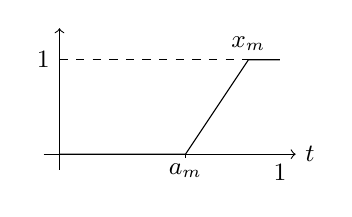
\begin{tikzpicture}[scale=1]
			\draw[->] (-0.2,0) -- (3,0) node[right] {\small $t$};
			\draw[->] (0,-0.2) -- (0,1.6);
			\draw (0,0) -- (1.6,0) -- (2.4,1.2) -- (2.8,1.2);
			\draw[dashed] (0,1.2) -- (2.4,1.2);
			\draw[dashed] (1.6,0) -- (1.6,-0.05);
			\draw (0,1.2) node[left] {\small $1$};
			\draw (1.6,0) node[below] {\small $a_m$};
			\draw (2.8,0) node[below] {\small $1$};
			\draw (2.4,1.4) node {\small $x_m$};
		\end{tikzpicture}
	\end{center}
	Suponha, sem perda de generalidade, que $n>m$. Como $a_n-a_m=\frac{1}{2m}-\frac{1}{2n}$, segue que
	$$d(x_n,x_m)=\frac14\left(\frac1m-\frac1n\right)<\eps\text{,}$$
	logo $(x_m)$ é de Cauchy em relação à métrica $L^1$. Entretanto $(x_m)$ converge, em relação a essa
	métrica, para
	$$x(t)=\begin{cases}0\text{,} & t\in[0,1)\text{,} \\ 1\text{,} & t=1\text{,}\end{cases}$$
	que não é contínua e, portanto, não pertence a $C[0,1]$.
\end{myproof}

\qslista{35}{Sejam $X$ o conjunto das funções $f:[0,1]\to\bbR$ contínuas e
$d(x,y)=\int_0^1|x(t)-y(t)|\,dt$. Mostre que $(X,d)$ não é completo.}
\nt{Cf. exemplo anterior, já demonstrado.}

\qslista{36}{Seja $Y=\{x\in C[a,b] \mid x(a)=x(b)\}\subset C[a,b]$. Mostre que $Y$ é
completo.}

\qslista{47}{Mostre que $C[a,b]$ não é completo em relação à norma $\|x\|_1=\int_a^b
|x(t)|\,dt$. Mostre também que existe $C>0$ tal que $\|x\|_1\leq C\|x\|_\infty$, $\forall x\in C[a,b]$,
sendo $\|\cdot\|_\infty$ a norma usual de $C[a,b]$. Pode existir $C>0$ tal que $\|x\|_\infty\leq
C\|x\|_1$, $\forall x\in C[a,b]$?}

\qslista{48}{Mostre que $C^1[a,b]=\{f:[a,b]\to\bbR \mid f \text{ é continuamente
diferenciável}\}$ é um espaço de Banach com a norma
$$\|x\|=\max_{t\in[a,b]}|x(t)|+\max_{t\in[a,b]}|x'(t)|\text{.}$$}

\subsection{Completude de $\ell^p$}

\mprop{$\ell^p$ é completo, $1\leq p<\infty$}{}
\begin{myproof}
	Seja $(x_n)\subset\ell^p$ de Cauchy, $x_n=\big(x_1^{(n)},x_2^{(n)},x_3^{(n)},\dots\big)$. Então
	$\forall\eps>0\ \exists N(\eps)\in\bbN$ tal que
	$$n,m\geq N \implies d(x_n,x_m)=\sum_{k\in\bbN}\big|x_k^{(n)}-x_k^{(m)}\big|^p<\eps^p\text{.}$$
	Note que, para cada $k\in\bbN$, $\big|x_k^{(n)}-x_k^{(m)}\big|^p\leq d(x_n,x_m)<\eps^p$, logo
	$\big(x_k^{(n)}\big)_{n\in\bbN}$ é de Cauchy em $\bbR$, i.e.,
	\begin{align}
		x_k^{(n)}\xrightarrow{n\to\infty}x_{(k)}\text{.}
	\end{align}
	Com isso definimos $x=\big(x_{(k)}\big)_{k\in\bbN}$ e notamos que $x_n\xrightarrow{n\to\infty}x$.
	Verifiquemos que $x\in\ell^p$:
	$$\sum_{k\in\bbN}\big|x_{(k)}\big|^p=\sum_{k\in\bbN}\Big|\big(x_{(k)}-x_k^{(n)}\big)-\big(-x_k^{(n)}\big)\Big|^p$$
	$$\implies \|x\|_{\ell^p}=d(x-x_n,x_n)\leq d(x,x_n)+\|x_n\|_{\ell^p}\text{,}\quad \forall n\in\bbN\text{.}$$
	Como $x_n\xrightarrow{n\to\infty}x$, dado $\eps_0>0$ existe $N_0\in\bbN$ tal que
	$\|x\|_{\ell^p}<\eps_0+\|x_{N_0}\|_{\ell^p}<+\infty$, pois $(x_n)\subset\ell^p$. Ou seja, sequências de
	Cauchy em $\ell^p$ convergem em $\ell^p$.
\end{myproof}

\subsection{Subespaços Fechados de Espaços Completos}

\nt{Requisitos para o Teorema do Ponto Fixo de Banach.}

\thm{}{Considere $(X,d)$ espaço métrico completo e $F\subset X$. $F$ é fechado $\iff$ $F$ é completo em
relação à métrica induzida de $X$.}
\begin{myproof}
	($\Rightarrow$) Seja $(x_n)\subset F$ sequência de Cauchy. Em particular $(x_n)$ é Cauchy em $X$.
	Assim, $x_n\xrightarrow{n\to\infty}x\in X$. Mas $F$ é fechado e, por consequência, $x\in F$. Logo $F$
	é completo.

	($\Leftarrow$) Suponha $F$ completo. Considere $x\in\bar F$. Logo existe $(x_n)\subset F$ tal que
	$x_n\xrightarrow{(X,d)}x$ e, por consequência, $(x_n)$ é de Cauchy em $F$. Como $F$ é completo, segue
	que existe $y\in F$ tal que $x_n\xrightarrow{(X,d)}y$. Da unicidade do limite em espaços métricos,
	segue que $x=y \implies \bar F=F \implies F$ é fechado.
\end{myproof}

\qslista{32}{Seja $c_{00}\subset\ell^\infty$ o subespaço de todas as sequências com no
máximo uma quantidade finita de termos não nulos. Mostre que $c_{00}$ não é completo em relação à métrica
induzida de $\ell^\infty$.}

\qslista{33}{Sejam $c$ e $c_0$ os subespaços de $\ell^\infty$ formados, respectivamente,
por todas as sequências convergentes e por todas as sequências convergentes para zero. Mostre que $c$ e
$c_0$ são fechados em $\ell^\infty$, logo são completos. Mostre também que esses subespaços são
separáveis.}

\qslista{45}{Sejam $Y$ e $Z$ subespaços de um espaço de Banach $X$. Suponha que existe
$C>0$ tal que
$$\text{dist}(x,Y\cap Z)\leq C\,\text{dist}(x,Y)\text{,}\quad \forall x\in X\text{,}$$
mostre que $Y+Z$ é fechado.}

\chapter{Contrações, Completamento e Espaços de Banach}

\section{Contrações e o Teorema do Ponto Fixo de Banach}

\dfn{Contração}{Sejam $(X,d_1)$, $(Y,d_2)$ espaços métricos. Uma contração de $X$ em $Y$ é uma aplicação
$T:X\to Y$ tal que existe $0<\alpha<1$ satisfazendo
$$d_2(T(x),T(y))\leq \alpha\, d_1(x,y)\text{,}\quad \forall x,y\in X\text{.}$$}

\nt{Toda contração é uniformemente contínua.}

\thm{Ponto Fixo de Banach}{Sejam $(X,d)$ espaço métrico completo e $T:X\to X$ uma contração. Então existe
um único ponto $x\in X$ tal que $Tx=x$.}
\begin{myproof}
	Seja $\alpha\in(0,1)$ tal que $d(T(x),T(y))\leq\alpha\, d(x,y)$, $\forall x,y\in X$.

	Seja $x_0\in X$ e defina a sequência $(x_n)=(x_0,x_1,\dots,x_n)$, $x_n=T(x_{n-1})=T^n(x_0)$,
	$\forall n\in\bbN$. Para cada $m\in\bbN$,
	$$d(x_m,x_{m+1})\leq \alpha\, d(x_{m-1},x_m)\leq\dots\leq \alpha^m d(x_0,x_1)\text{.}$$
	Para $n,m\in\bbN$ com $m>n$,
	\begin{align*}
		d(x_n,x_m) & \leq \sum_{k=1}^{m-n}d(x_{n+k-1},x_{n+k}) \leq \sum_{k=1}^{m-n}\alpha^{n+k-1}d(x_0,x_1) \\
		           & = \alpha^n\left(\sum_{k=1}^{m-n}\alpha^{k-1}\right)d(x_0,x_1) < \alpha^n\cdot\frac{1}{1-\alpha}\,d(x_0,x_1)\xrightarrow{n\to\infty}0\text{.}
	\end{align*}
	Portanto $(x_n)$ é de Cauchy. Como $X$ é completo, existe $x\in X$ tal que $x_n\to x$. Note que
	$$T(x)=T\Big(\lim_n x_n\Big)=\lim_n T(x_n)=\lim_n x_{n+1}=x\text{.}$$

	\textit{Unicidade:} suponha $x,y\in X$ tais que $T(x)=x$, $T(y)=y$. Então
	$$d(x,y)=d(Tx,Ty)\leq\alpha\, d(x,y) \implies (1-\alpha)\,d(x,y)\leq 0 \implies d(x,y)=0 \implies x=y\text{.}$$
\end{myproof}

\qslista{42}{Sejam $(X,d)$ um espaço métrico completo e $T$ uma aplicação contínua em $X$.
Supondo que $T^N$ é uma contração para algum $N\in\bbN$, prove que $T$ possui um único ponto fixo.}

\section{Aplicação: Existência e Unicidade Local de EDOs}

Sejam $\Omega\subset\bbR^{n+1}$ aberto e $f:\Omega\to\bbR^n$ contínua tal que existe $M>0$ satisfazendo
$$(A)\qquad |f(t,x_1)-f(t,x_2)|\leq M|x_1-x_2|\text{,}\quad \forall (t,x_1),(t,x_2)\in\Omega\text{.}$$

Considere a EDO
$$(1)\qquad \frac{d}{dt}x=f(t,x)\text{.}$$
Uma solução dessa EDO passando por $(t_0,x_0)$ é uma função $\varphi:J\to\bbR^n$ que satisfaz
$\varphi(t_0)=x_0$ e $\dfrac{d\varphi(t)}{dt}=f(t,\varphi(t))$, $\forall t\in J$ (algum aberto $J$,
$t_0\in J$). Essa $\varphi$ pode ser escrita, equivalentemente, como
$$\varphi(t)=x_0+\int_{t_0}^{t}f(s,\varphi(s))\,ds\text{.}$$

\thm{Teorema de Picard}{Seja $f$ como acima. Para cada $(t_0,x_0)\in\Omega$, a EDO $(1)$ possui uma única
solução local passando por $(t_0,x_0)$.}
\begin{myproof}
	Seja $\tilde\Omega\subset\Omega$ aberto tal que $f$ é limitada em $\tilde\Omega$, i.e., existe $A>0$
	tal que $|f(t,x)|\leq A$, $\forall(t,x)\in\tilde\Omega$.

	Tome $\delta>0$ tal que $R=[t_0-\delta,t_0+\delta]\times B[x_0,\delta]\subset\tilde\Omega$, com
	$\delta<1$ e $M\delta<1$. Denote $J=[t_0-\delta,t_0+\delta]$ e defina
	$$B=\Big\{\psi:J\to\bbR^n \ \Big|\ \psi \text{ contínua},\ \psi(t_0)=x_0,\ |\psi(t)-x_0|\leq A\delta,\ \forall t\in J\Big\}\text{.}$$

	Vejamos que $B\subset C(J,\bbR^n)$ é fechado, sendo $C(J,\bbR^n)$ completo com a métrica
	$d_\infty(x,y)=\sup_{t\in J}|x(t)-y(t)|$. Seja $(\psi_n)\subset B$ tal que $\psi_n\to\psi$ em
	$C(J,\bbR^n)$; em particular $\psi_n\to\psi$ uniformemente, logo $\psi$ é contínua. De fato,
	$|\psi_n(t_0)-\psi(t_0)|\leq d_\infty(\psi_n,\psi)\to 0 \implies \psi(t_0)=x_0$, e
	$$|\psi(t)-x_0|=\lim_n|\psi_n(t)-x_0|\leq \lim_n A\delta = A\delta\text{,}$$
	logo $\psi\in B$ e $B$ é fechado. Como $B\subset C(J,\bbR^n)$ é fechado e $C(J,\bbR^n)$ é completo, $B$
	é completo com a métrica induzida.

	Considere $T:B\to C(J,\bbR^n)$ dada por $(T\psi)(t)=x_0+\int_{t_0}^{t}f(s,\psi(s))\,ds$. Vejamos que
	$T:B\to B$:
	\begin{itemize}
		\item $(T\psi)(t_0)=x_0$;
		\item $|(T\psi)(t)-x_0|\leq \int_{t_0}^{t}A\,ds=A(t-t_0)<A\delta$.
	\end{itemize}

	\textit{Afirmação: $T$ é contração.} De fato,
	\begin{align*}
		|(T\psi_1)(t)-(T\psi_2)(t)| & \leq \left|\int_{t_0}^{t}f(s,\psi_1(s))-f(s,\psi_2(s))\,ds\right|                     \\
		                            & \leq \int_{t_0}^{t}|f(s,\psi_1(s))-f(s,\psi_2(s))|\,ds \leq M\int_{t_0}^{t}|\psi_1(s)-\psi_2(s)|\,ds \\
		                            & \leq \underbrace{M\delta}_{<1}\, d_\infty(\psi_1,\psi_2)\text{.}
	\end{align*}
	Portanto $T:B\to B$ é contração. Pelo Teorema do Ponto Fixo de Banach, existe um único $\psi\in B$ tal
	que $T(\psi)=\psi$, ou seja, existe uma única
	$$\varphi(t)=x_0+\int_{t_0}^{t}f(s,\varphi(s))\,ds$$
	que é a solução local de $(1)$ passando por $(t_0,x_0)$.
\end{myproof}

\section{Completamento de Espaços Métricos}

\dfn{Imersão Isométrica e Isometria}{Sejam $(X,d_1)$, $(Y,d_2)$ espaços métricos. Uma imersão isométrica
entre $X$ e $Y$ é uma aplicação $T:X\to Y$ tal que $d_2(T(x),T(y))=d_1(x,y)$, $\forall x,y\in X$. Quando
$T$ é bijetiva, dizemos que $T$ é uma isometria e que $X$ e $Y$ são isométricos.}

\nt{Toda imersão isométrica é injetiva.}

\dfn{Completamento}{Seja $(X,d)$ espaço métrico. Um completamento de $X$ é um par $(\hat X,\varphi)$ tal
que $\hat X=(\hat X,\hat d)$ é espaço métrico completo e $\varphi:X\to\hat X$ é uma imersão isométrica tal
que $\overline{\varphi(X)}=\hat X$.}

\thm{Teorema do Completamento}{Todo espaço métrico $(X,d)$ admite um completamento. Esse completamento é
único a menos de isometrias.}
\begin{myproof}
	Organizamos a demonstração em quatro etapas: (a) construção de $(\hat X,\hat d)$; (b) definição de
	$T:X\to\hat X$ imersão isométrica com $\overline{T(X)}=\hat X$; (c) $(\hat X,\hat d)$ é completo; (d)
	unicidade de $\hat X$ a menos de isometria.

	\textbf{(a)} Seja $X^*$ o conjunto das sequências de Cauchy em $X$. \textit{Afirmação:}
	$(x_n),(y_n)\in X^* \implies d(x_n,y_n)$ converge em $\bbR$. De fato,
	$|d(x_n,y_n)-d(x_m,y_m)|\leq d(x_n,x_m)+d(y_n,y_m)$, logo $(d(x_n,y_n))_{n\in\bbN}$ é de Cauchy em
	$\bbR$, portanto convergente.

	Definimos em $X^*$ a relação $(x_n)\sim(y_n) :\iff d(x_n,y_n)\to 0$, $n\to\infty$, que é reflexiva,
	simétrica (imediato) e transitiva (pela desigualdade triangular), i.e., uma relação de equivalência.
	Seja $\hat x=[x]$, $x=(x_n)\in X^*$, a classe de equivalência de $x$, e $\hat X=X^*/\!\sim$.

	Definimos $\hat d:\hat X\times\hat X\to[0,+\infty)$, $(\hat x,\hat y)\mapsto \hat
	d(\hat x,\hat y)=\lim_n d(x_n,y_n)$, $(x_n)\in\hat x$, $(y_n)\in\hat y$. $\hat d$ está bem definida:
	se $(x_n),(x_n')\in\hat x$ e $(y_n),(y_n')\in\hat y$, então
	$d(x_n',y_n')\leq d(x_n',x_n)+d(x_n,y_n)+d(y_n,y_n')$, logo $\lim_n d(x_n',y_n')\leq \lim_n
	d(x_n,y_n)$ e, por simetria, vale a igualdade.

	$\hat d$ é métrica: $(M_1)$ $\hat d(\hat x,\hat y)=0 \iff \lim_n d(x_n,y_n)=0 \iff (x_n)\sim(y_n) \iff
	\hat x=\hat y$; $(M_2)$ segue da simetria de $d$; $(M_3)$ dados $\hat x,\hat y,\hat z\in\hat X$,
	$d(x_n,y_n)\leq d(x_n,z_n)+d(z_n,y_n)$ e, passando ao limite, $\hat d(\hat x,\hat y)\leq \hat
	d(\hat x,\hat z)+\hat d(\hat z,\hat y)$. Logo $(\hat X,\hat d)$ é espaço métrico.

	\textbf{(b)} Definimos $T:X\to\hat X$, $x\mapsto T(x)=[(x,x,x,\dots)]$. Então
	$\hat d(T(x),T(y))=\lim_n d(x,y)=d(x,y)$, logo $T$ preserva a métrica.

	$\overline{T(X)}=\hat X$: dado $\eps>0$ e $\hat x=[(x_n)]\in\hat X$, como $(x_n)\in X^*$ é de Cauchy,
	existe $N\in\bbN$ tal que $d(x_n,x_N)<\eps/2$, $\forall n>N$. Seja $y=[(x_N,x_N,\dots)]\in T(X)$. Logo
	$\hat d(\hat x,y)=\lim_n d(x_n,x_N)\leq \eps/2<\eps$, i.e., $\hat x\in\overline{T(X)}$. Portanto
	$\overline{T(X)}=\hat X$.

	\textbf{(c)} Seja $(\hat x_n)$ sequência de Cauchy em $\hat X$. Como $\overline{T(X)}=\hat X$, para
	cada $n\in\bbN$ tome $\hat z_n\in T(X)$ tal que $\hat d(\hat z_n,\hat x_n)<1/n$, $\hat z_n=T(z_n)$,
	$z_n\in X$. Verifiquemos que $(z_n)$ é de Cauchy em $X$:
	$$d(z_n,z_m)=\hat d(\hat z_n,\hat z_m)\leq \hat d(\hat z_n,\hat x_n)+\hat d(\hat x_n,\hat x_m)+\hat
	d(\hat x_m,\hat z_m) < \frac1n+\eps+\frac1m\text{,}\quad \forall n,m\geq N\text{.}$$
	Seja $\hat x=[(z_n)]\in\hat X$. Então
	$$\hat d(\hat x,\hat x_n)\leq \hat d(\hat x,\hat z_n)+\hat d(\hat z_n,\hat x_n) < \Big(\lim_{m\to\infty}d(z_m,z_n)\Big)+\frac1n \xrightarrow{n\to\infty}0\text{,}$$
	logo $\hat x_n\to\hat x$ em $\hat X$, i.e., $(\hat X,\hat d)$ é completo.

	\textbf{(d)} Sejam $(\hat X,\hat d)$ e $(\tilde X,\tilde d)$ completos, com $T:X\to\hat X$ e
	$S:X\to\tilde X$ imersões isométricas satisfazendo $\overline{T(X)}=\hat X$, $\overline{S(X)}=\tilde
	X$. Usamos o seguinte resultado auxiliar: se $(X,d)$ é métrico, $(Y,\tilde d)$ é métrico completo,
	$D\subset X$ com $\bar D=X$ e $\varphi:D\to Y$ é imersão isométrica, então $\varphi$ se estende
	unicamente a uma imersão isométrica $F:X\to Y$ (ver Elon Lages Lima, \emph{Espaços Métricos},
	pág.\ 178).

	Para cada $y\in T(X)$, existe um único $x\in X$ tal que $y=T(x)$; definimos
	$\psi:T(X)\to\tilde X$, $y\mapsto\psi(y)=S(x)$. $\psi$ está bem definida e preserva distância: se
	$y_i=T(x_i)$, $i=1,2$,
	$$\tilde d(\psi(y_1),\psi(y_2))=\tilde d(S(x_1),S(x_2))=d(x_1,x_2)=\hat d(T(x_1),T(x_2))=\hat d(y_1,y_2)\text{.}$$
	Pelo resultado auxiliar, existe uma única $F:\hat X\to\tilde X$ isométrica tal que $F|_{T(X)}=\psi$;
	verificando que $F$ é bijetiva, concluímos que $\hat X$ e $\tilde X$ são isométricos.
\end{myproof}

\ex{Completamentos usuais}{
	\begin{enumerate}
		\item $(\bbR,|\cdot|)$ é o completamento de $(\bbQ,|\cdot|)$.
		\item Considerando $C[a,b]$ com a métrica $d_p(x,y)=\left(\int_a^b|x(t)-y(t)|^p\,dt\right)^{1/p}$,
		      $1\leq p<\infty$, o espaço $L^p[a,b]$ é o completamento de $C[a,b]$ com essa métrica.
	\end{enumerate}}

\qslista{37}{Sejam $X$ um conjunto e $(M,d)$ um espaço métrico. Considere
$B(X,M)=\{f:X\to M \mid f \text{ é limitada}\}$ com a métrica $d_0(f,g)=\sup_{x\in X}d(f(x),g(x))$. Prove
que existe uma isometria entre os espaços $B(X\times Y,M)$ e $B(X,B(Y,M))$.}

\qslista{40}{Se $X_1$ e $X_2$ são espaços métricos isométricos e $X_1$ é completo, mostre
que $X_2$ também é completo.}

\qslista{41}{Mostre que os espaços $C[a,b]$ e $C[0,1]$ são isométricos.}

\section{Completamento de Espaços Normados}

\thm{Completamento de um Espaço Normado}{Seja $(E,\|\cdot\|)$ espaço normado. Então existe um espaço de
Banach $(\hat E,\|\cdot\|_{\hat E})$ e uma imersão isométrica linear $T:E\to\hat E$
($\|T(x)\|_{\hat E}=\|x\|_E$, $\forall x\in E$) tal que $\overline{T(E)}=\hat E$. O espaço
$(\hat E,\|\cdot\|_{\hat E})$ é único a menos de isometrias.}

\nt{A construção de $(\hat E,\|\cdot\|_{\hat E})$ é análoga à do completamento de espaços métricos,
aplicada à métrica induzida pela norma de $E$.}

\section{Séries em Espaços de Banach}

\dfn{Convergência Absoluta}{Dizemos que a série $\sum_{k\geq 1}x_k$, $x_k\in E$, é absolutamente
convergente quando $\sum_k\|x_k\|$ converge em $\bbR$.}

\thm{}{$(E,\|\cdot\|)$ é de Banach sse toda série absolutamente convergente em $E$ converge em $E$.}
\begin{myproof}
	($\Rightarrow$) Suponha $E$ Banach. Seja $(x_n)\subset E$ tal que $\sum_{n=1}^{\infty}\|x_n\|<\infty$.
	Considere $S_N=\sum_{k=1}^{N}x_k$. Vejamos que $(S_N)$ é de Cauchy em $E$: para $N>M$,
	$$\|S_N-S_M\|\leq \sum_{k=M+1}^{N}\|x_k\|\xrightarrow{M,N\to\infty}0\text{,}$$
	logo $(S_N)$ converge em $E$.

	($\Leftarrow$) Seja $(x_n)\subset E$ sequência de Cauchy. Para cada $j\in\bbN$, existe $n_j\in\bbN$
	tal que $\|x_n-x_m\|<1/2^j$, $\forall n,m\geq n_j$; podemos supor $(n_j)$ crescente. Defina
	$y_1=x_{n_1}$, $y_j=x_{n_j}-x_{n_{j-1}}$, $j\geq 2$, de modo que $\sum_{j=1}^{k}y_j=x_{n_k}$. Note que
	$$\sum_{j=1}^{k}\|y_j\| = \|x_{n_1}\|+\sum_{j=2}^{k}\|x_{n_j}-x_{n_{j-1}}\| < \|x_{n_1}\|+\sum_{j\in\bbN}\frac{1}{2^j}=\|x_{n_1}\|+1\text{,}$$
	logo $\sum_{j=1}^{\infty}\|y_j\|<\infty$. Por hipótese, a série $\sum_{j=1}^{\infty}y_j$ converge, i.e.,
	$(x_{n_k})$ converge em $E$. Como $(x_n)$ é Cauchy e possui subsequência convergente, $(x_n)$ converge
	em $E$.
\end{myproof}

\section{Base, Dimensão e Base de Schauder}

Seja $X$ espaço vetorial sobre $\bbK$ ($\bbR$ ou $\bbC$).

\dfn{Independência Linear e Base de Hamel}{$B\subset X$ é linearmente independente (LI) quando, para todo
$L\subset B$ finito, $\sum_{\ell\in L}\alpha_\ell\,\ell=0 \implies \alpha_\ell=0$, $\forall \ell\in L$; caso
contrário, $B$ é linearmente dependente (LD). O \emph{span} de $B$ é
$\text{Span}\,B=\big\{\sum_{k=1}^{M}\alpha_kx_k \mid \alpha_k\in\bbK,\ M\in\bbN,\ x_k\in B\big\}$. Uma base
de $X$ (ou base de Hamel) é um conjunto $B\subset X$ LI tal que $\text{Span}\,B=X$.}

\dfn{Dimensão Finita e Infinita}{Dizemos que $X$ tem dimensão finita quando existe $B\subset X$ finito,
LI, tal que qualquer outro conjunto com mais elementos que $B$ é LD (nesse caso, qualquer $A\subset X$ LI
possui no máximo $|B|$ elementos). Caso contrário, $X$ tem dimensão infinita.}

\nt{A existência de uma base de Hamel para todo espaço vetorial não nulo é demonstrada na Seção 4.2
(Teorema 4.2.1), via o Lema de Zorn.}

\dfn{Base de Schauder}{Seja $(E,\|\cdot\|)$ espaço normado. Se existe $(e_n)\subset E$ LI tal que, para
todo $x\in E$, existe uma sequência de escalares $(\alpha_n)$ satisfazendo
$$\left\|x-\sum_{j=1}^{n}\alpha_je_j\right\|\xrightarrow{n\to\infty}0\text{,}$$
dizemos que $(e_n)$ é uma base de Schauder para $E$.}

\ex{Base canônica de $\ell^p$}{$E=\ell^p$, $(e_n)$ tal que $(e_n)_j=\begin{cases}0\text{,}&j\neq n\text{,}\\1\text{,}&j=n\text{.}\end{cases}$
Dado $x=(x_n)\in\ell^p$,
$$\left\|x-\sum_{k=1}^{N}x_ke_k\right\|_p^p=\sum_{k=N+1}^{\infty}|x_k|^p\xrightarrow{N\to\infty}0\text{,}$$
logo $(e_n)$ é base de Schauder para $\ell^p$.}

\thm{}{Se $(E,\|\cdot\|)$ possui base de Schauder, então $E$ é separável.}
\begin{myproof}
	Seja $(e_n)$ base de Schauder de $E$ e considere
	$$D=\left\{\sum_{j=1}^{n}q_je_j \ \middle|\ n\in\bbN,\ q_j\in\bbQ \text{ (ou } \bbQ+i\bbQ \text{, no
	caso complexo)}\right\}\text{,}$$
	que é enumerável, por ser uma união enumerável (em $n$) de conjuntos enumeráveis ($\bbQ^n$).

	Vejamos que $\bar D=E$. Dados $x\in E$ e $\eps>0$, pela definição de base de Schauder existe
	$N\in\bbN$ tal que $\|x-\sum_{j=1}^{N}\alpha_je_j\|<\eps/2$. Pela densidade de $\bbQ$ em $\bbR$,
	escolha $q_j\in\bbQ$ tal que $|\alpha_j-q_j|<\dfrac{\eps}{2N\max_j\|e_j\|}$, $j=1,\dots,N$; então
	$$\left\|\sum_{j=1}^{N}(\alpha_j-q_j)e_j\right\|\leq\sum_{j=1}^{N}|\alpha_j-q_j|\,\|e_j\|<\frac{\eps}{2}\text{.}$$
	Logo, com $y=\sum_{j=1}^{N}q_je_j\in D$,
	$$\|x-y\|\leq\left\|x-\sum_{j=1}^{N}\alpha_je_j\right\|+\left\|\sum_{j=1}^{N}(\alpha_j-q_j)e_j\right\|<\frac{\eps}{2}+\frac{\eps}{2}=\eps\text{,}$$
	i.e., $x\in\bar D$. Portanto $D$ é enumerável e denso em $E$, logo $E$ é separável.
\end{myproof}

\nt{Em particular, $\ell^\infty$ não possui base de Schauder, pois $\ell^\infty$ não é separável.}

\qslista{44}{Mostre que todo espaço normado que possui base de Schauder é separável.}
\nt{Cf. Teorema 2.6.1, já demonstrado acima.}

\chapter{Dimensão Finita e Operadores Lineares Limitados}

\section{Normas Equivalentes}

\dfn{Normas Equivalentes}{Seja $X$ espaço vetorial. Duas normas $\|\cdot\|_1,\|\cdot\|_2$ em $X$ são
equivalentes quando existem $\alpha,\beta>0$ tais que
$$\alpha\|x\|_2\leq\|x\|_1\leq\beta\|x\|_2\text{,}\quad\forall x\in X\text{.}$$}

\nt{Normas equivalentes geram os mesmos abertos de $X$; a recíproca não vale em geral, i.e., existem
espaços métricos com os mesmos abertos cujas métricas não provêm de normas equivalentes.}

\qslista[2]{2}{Se $\dim X<+\infty$, então todas as normas em $X$ são equivalentes.}
\begin{myproof}
	Seja $\{e_1,\dots,e_n\}$ base de $X$ e $\|\cdot\|$ uma norma qualquer em $X$. Escrevendo
	$x=\sum_k\alpha_ke_k$, defina $\|x\|_1:=\sum_k|\alpha_k|$; como a equivalência de normas é
	transitiva, basta mostrar que $\|\cdot\|$ e $\|\cdot\|_1$ são equivalentes.

	Pela desigualdade triangular, $\|x\|\leq\sum_k|\alpha_k|\,\|e_k\|\leq\beta\|x\|_1$, onde
	$\beta:=\max_k\|e_k\|$. Considere agora $\varphi:\bbK^n\to\bbR$, $\varphi(\alpha)=\|\sum_k\alpha_ke_k\|$.
	Pela desigualdade anterior, $|\varphi(\alpha)-\varphi(\alpha')|\leq\beta\|\alpha-\alpha'\|_1$, logo
	$\varphi$ é (Lipschitz) contínua na topologia usual de $\bbK^n$.

	A esfera $S=\{\alpha\in\bbK^n \mid \|\alpha\|_1=1\}$ é compacta, e $\varphi(\alpha)>0$ para todo
	$\alpha\in S$, pois $\{e_k\}$ é LI. Por compacidade, $\varphi$ atinge um mínimo
	$c:=\min_{\alpha\in S}\varphi(\alpha)>0$. Dado $x\neq 0$, seja $t=\|\alpha\|_1>0$ e
	$\tilde\alpha=\alpha/t\in S$; por homogeneidade, $\|x\|=\varphi(\alpha)=t\,\varphi(\tilde\alpha)\geq
	tc=c\|x\|_1$.

	Logo $c\|x\|_1\leq\|x\|\leq\beta\|x\|_1$, $\forall x\in X$, i.e., $\|\cdot\|$ e $\|\cdot\|_1$ são
	equivalentes. Como $\|\cdot\|$ era arbitrária, todas as normas em $X$ são equivalentes entre si.
\end{myproof}

\qslista[2]{1}{Se $\dim X<\infty$, então toda transformação linear $T:X\to Y$ é contínua.}
\nt{Consequência da Questão 3.1.1 (acima): escrevendo $Tx=\sum_k\alpha_kTe_k$ na base de $X$ e usando a
equivalência entre $\|\cdot\|$ e $\|\cdot\|_1:=\sum_k|\alpha_k|$, obtém-se $\|Tx\|\leq M\|x\|_1\leq
MC\|x\|$.}

\qslista{26}{Dizemos que duas normas $\|\cdot\|_0$ e $\|\cdot\|_1$ são equivalentes num
espaço vetorial $V$ se existem constantes $C_1,C_2>0$ tais que
$$C_1\|x\|_1\leq \|x\|_0\leq C_2\|x\|_1\text{,}\quad \forall x\in V\text{.}$$
Mostre que, se $V$ tem dimensão finita, então todas as normas são equivalentes.}
\nt{Cf. Questão 3.1.1, já demonstrada acima.}

\section{Subespaços de Dimensão Finita}

\mprop{}{Seja $(X,\|\cdot\|)$ espaço normado e $\{x_1,\dots,x_n\}\subset X$ linearmente independente.
Então existe $c>0$ tal que
$$\left\|\sum_{k=1}^{n}\alpha_kx_k\right\|\geq c\sum_{k=1}^{n}|\alpha_k|\text{,}\quad \forall
(\alpha_k)_{k=1}^{n}\subset\bbK^n\text{.}$$}

\begin{myproof}
	Considere $\varphi:\bbK^n\to\bbR$, $\varphi(\alpha)=\big\|\sum_k\alpha_kx_k\big\|$. Pela desigualdade
	triangular, $|\varphi(\alpha)-\varphi(\alpha')|\leq\big(\max_k\|x_k\|\big)\|\alpha-\alpha'\|_1$, logo
	$\varphi$ é contínua na topologia usual de $\bbK^n$. A esfera $S=\{\alpha\in\bbK^n \mid
	\sum_k|\alpha_k|=1\}$ é compacta, e $\varphi(\alpha)>0$ para todo $\alpha\in S$, pois
	$\{x_1,\dots,x_n\}$ é LI (nenhuma combinação não trivial se anula). Por compacidade, $\varphi$ atinge
	um mínimo $c:=\min_{\alpha\in S}\varphi(\alpha)>0$.

	Dado $(\alpha_k)_{k=1}^{n}\neq 0$, seja $t=\sum_k|\alpha_k|>0$ e $\tilde\alpha=\alpha/t\in S$; por
	homogeneidade da norma,
	$$\left\|\sum_k\alpha_kx_k\right\|=\varphi(\alpha)=t\,\varphi(\tilde\alpha)\geq tc=c\sum_k|\alpha_k|\text{,}$$
	e para $(\alpha_k)=0$ a desigualdade é trivial.
\end{myproof}

\thm{}{Seja $X$ espaço normado e $Y\subset X$ com $\dim Y<\infty$. Então $Y$ é completo.}
\begin{myproof}
	Seja $(y_n)\subset Y$ sequência de Cauchy e $\{e_1,\dots,e_N\}$ base de $Y$. Para cada $n\in\bbN$,
	escrevemos $y_n=\sum_{k=1}^{N}\alpha_k^{(n)}e_k$. Dado $\eps>0$, existe $n_0\in\bbN$ tal que
	$\|y_n-y_m\|<\eps$, $\forall n,m\geq n_0$.

	Pela proposição anterior, para $n,m\geq n_0$,
	$$\eps>\|y_n-y_m\|=\left\|\sum_{j=1}^{N}\big(\alpha_j^{(n)}-\alpha_j^{(m)}\big)e_j\right\|\geq
	c\sum_{j=1}^{N}\big|\alpha_j^{(n)}-\alpha_j^{(m)}\big|\text{,}$$
	logo $\big|\alpha_j^{(n)}-\alpha_j^{(m)}\big|<\eps/c$ para cada $j\in\{1,\dots,N\}$, i.e.,
	$\big(\alpha_j^{(k)}\big)_{k\in\bbN}$ é de Cauchy em $\bbR$. Portanto existe $\alpha_j\in\bbR$ tal que
	$\alpha_j^{(n)}\to\alpha_j$. Seja $y=\sum_{j=1}^{N}\alpha_je_j$. Com isso,
	$$\|y_n-y\|=\left\|\sum_{j=1}^{N}\big(\alpha_j^{(n)}-\alpha_j\big)e_j\right\|\leq
	\sum_{j=1}^{N}\big|\alpha_j^{(n)}-\alpha_j\big|\,\|e_j\|\xrightarrow{n\to\infty}0\text{.}$$
\end{myproof}

\cor{}{Seja $X$ espaço normado e $Y\subset X$ com $\dim Y<\infty$. Então $Y$ é fechado em $X$.}

\section{Compacidade em Dimensão Finita}

\thm{}{Seja $X$ espaço normado com $\dim X<\infty$. Dado $M\subset X$, são equivalentes: (i) $M$ é
sequencialmente compacto; (ii) $M$ é fechado e limitado.}
\begin{myproof}
	$(i)\Rightarrow(ii)$: Seja $x\in\bar M$. Existe $(x_n)\subset M$ tal que $x_n\to x$ em $X$. Como $M$ é
	sequencialmente compacto, existe $(y_n)\subset(x_n)$ tal que $y_n\to y\in M$; pela unicidade do
	limite, $x=y\in M$. Logo $M=\bar M$.

	Vejamos que $M$ é limitado. Suponha o contrário: $\forall n\in\bbN$, existe $x_n\in M$ tal que
	$\|x_n\|>n$. Então $(x_n)\subset M$ não possui subsequência convergente, uma contradição. (Note que
	esta implicação não usa $\dim X<\infty$.)

	$(ii)\Rightarrow(i)$: Seja $N=\dim X$ e $\{e_1,\dots,e_N\}$ base de $X$. Dada $(x_n)\subset M$, para
	cada $n\in\bbN$, $x_n=\sum_{k=1}^{N}\alpha_k^{(n)}e_k$. Como $M$ é limitado, existe $K>0$ tal que
	$\|x_n\|\leq K$, $\forall n\in\bbN$. Pela proposição da Seção 3.2,
	$$K>\|x_m\|=\left\|\sum_{j=1}^{N}\alpha_j^{(m)}e_j\right\|\geq c\sum_{j=1}^{N}\big|\alpha_j^{(m)}\big|\text{,}$$
	logo $\big|\alpha_j^{(m)}\big|<K/c$, $\forall m\in\bbN$, $\forall j\in\{1,\dots,N\}$, i.e.,
	$\big(\alpha_j^{(m)}\big)_{m\in\bbN}$ é limitada para todo $j$.

	Pelo Teorema de Bolzano--Weierstrass, extraímos sucessivamente (para $j=1,\dots,N$) subsequências
	$$\big(x_{n_k}^{(N)}\big)_{k\in\bbN}\subseteq\big(x_{n_k}^{(N-1)}\big)_{k\in\bbN}\subseteq\dots\subseteq(x_n)$$
	tais que, para cada $j$, o $j$-ésimo coeficiente converge: $\alpha_j^{(n_k,j)}\xrightarrow{k\to\infty}\alpha_j$. Com isso,
	$$x_{n_k}^{(N)}=\sum_{j=1}^{N}\alpha_j^{(n_k,N)}e_j \xrightarrow{k\to\infty} \sum_{j=1}^{N}\alpha_je_j=:x
	\quad\text{em } X\text{.}$$
	Como $M$ é fechado, $x\in M$.
\end{myproof}

\nt{Se $\dim X=\infty$, em geral $(ii)$ não implica $(i)$. Exemplo: $X=\ell^p$, $1\leq p<\infty$, com
$(e_n)$ a base canônica ($\|e_n\|_p=1$, $\|e_n-e_m\|_p\geq 1$, $\forall n\neq m$). O conjunto
$M=\{e_n\mid n\in\bbN\}$ é limitado e fechado, mas não é compacto, pois $(e_n)$ não possui subsequência
convergente.}

\qslista{22}{Seja $(E,\|\cdot\|)$ um espaço normado de dimensão finita. Prove que um
subconjunto de $E$ é compacto se, e somente se, é fechado e limitado.}
\nt{Cf. Teorema 3.3.1, já demonstrado acima.}

\qslista{23}{Dê um exemplo de um subconjunto em um espaço normado que é fechado e
limitado, mas não é compacto.}
\nt{Cf. observação acima (base canônica de $\ell^p$).}

\section{Lema de Riesz}

\thm{Lema de Riesz}{Seja $X$ espaço normado e $Y,Z\subset X$ subespaços vetoriais com $Y$ fechado e
$Y\subsetneq Z$ (subespaço próprio). Para todo $\theta\in(0,1)$, existe $z\in Z$ tal que $\|z\|=1$ e
$\|z-y\|\geq\theta$, $\forall y\in Y$ (i.e., a distância de $z$ a $Y$, induzida pela norma, satisfaz
$D(z,Y)\geq\theta$).}
\begin{myproof}
	Seja $v\in Z\setminus Y$ arbitrário e $a:=D(v,Y)=\inf_{y\in Y}\|v-y\|>0$ (pois $Y$ é fechado e
	$v\notin Y$). Dado $\theta\in(0,1)$, existe $y_0\in Y$ tal que $a\leq\|v-y_0\|\leq a/\theta$.

	Seja $z=c(v-y_0)$, $c=1/\|v-y_0\|$; logo $\|z\|=1$. Para todo $y\in Y$,
	$$\|z-y\|=\|c(v-y_0)-y\|=|c|\,\big\|v-(y_0+c^{-1}y)\big\|\geq ca\geq\theta\text{,}$$
	pois $y_0+c^{-1}y\in Y$ (logo $\|v-(y_0+c^{-1}y)\|\geq a$) e $c\geq\theta/a$. Portanto
	$\inf_{y\in Y}\|z-y\|\geq\theta$.
\end{myproof}

\qslista[2]{3}{No Lema de Riesz, se $\dim Y=\infty$ o parâmetro $\theta$ não pode ser tomado igual
a $1$; se $\dim Y<\infty$, existe $z$ com $\|z\|=1$ e $\|z-y\|\geq1$ para todo $y\in Y$.}

\thm{}{Seja $X$ espaço normado. $\dim X<\infty \iff \overline{B}_1(0)=\{x\in X\mid \|x\|\leq 1\}$ é
compacta em $X$.}
\begin{myproof}
	($\Rightarrow$) Suponha $\dim X<\infty$. Pelas proposições anteriores, $\overline{B}_1(0)$ é fechada e
	limitada, logo compacta.

	($\Leftarrow$) Suponha $\overline{B}_1(0)$ compacta. Por contradição, suponha também $\dim X=\infty$.
	Seja $x_1\in X$ com $\|x_1\|=1$ e $X_1=\text{Span}\{x_1\}$, que é fechado e subespaço próprio de $X$.
	Pelo Lema de Riesz, existe $x_2\in X$ tal que $\|x_2\|=1$ e $\|x_2-x\|\geq 1/2$, $\forall x\in X_1$; em
	particular, $\|x_2-x_1\|\geq 1/2$.

	Seja $X_2=\text{Span}\{x_1,x_2\}$, fechado e subespaço próprio de $X$. Novamente pelo Lema de Riesz,
	existe $x_3\in X$ tal que $\|x_3\|=1$ e $\|x_3-x\|\geq 1/2$, $\forall x\in X_2$.

	Indutivamente, obtemos uma sequência $(x_n)$ satisfazendo $\|x_n\|=1$, $\forall n\in\bbN$, e
	$\|x_m-x_n\|\geq 1/2$, $\forall m\neq n$. Assim, $(x_n)\subset \overline{B}_1(0)$ não possui
	subsequência convergente, uma contradição.
\end{myproof}

\qslista{46}{Seja $X$ um espaço de Banach e $A\subset X$ um subconjunto compacto. O que
deve ocorrer quando $\text{int}(A)\neq\emptyset$?}

\section{Transformações Lineares Limitadas}

Sejam $X,Y$ espaços vetoriais.

\dfn{Transformação Linear}{Uma transformação linear de $X$ para $Y$ é uma aplicação $T:X\to Y$
satisfazendo, para cada $x,y\in X$ e $\lambda\in\bbK$,
$$T(x+y)=T(x)+T(y)\text{,}\qquad T(\lambda x)=\lambda T(x)\text{.}$$
Denotamos $N(T)=\{x\in X\mid Tx=0\}=T^{-1}(\{0\})$ (núcleo) e $R(T)=\{Tx\mid x\in X\}$ (imagem).}

\nt{$N(T)$ e $R(T)$ são subespaços vetoriais. Além disso:
\begin{itemize}
	\item se $\dim X<\infty$, então $\dim R(T)<\infty$;
	\item a inversa $T^{-1}:Y\to X$ existe se, e somente se, $N(T)=\{0\}$;
	\item se $T^{-1}$ existe, então ela também é linear;
	\item se $T^{-1}$ existe e $\dim X<\infty$, então $\dim R(T)=\dim X$.
\end{itemize}}

A partir daqui, $X,Y$ são espaços normados.

\dfn{Transformação Linear Limitada}{Uma transformação linear $T:X\to Y$ é limitada quando existe $c>0$
tal que $\|Tx\|_Y\leq c\|x\|_X$, $\forall x\in X$; equivalentemente, $\|Tx\|\leq c$, $\forall x\in X$ com
$\|x\|=1$.}

\thm{}{Sejam $X,Y$ normados e $T:X\to Y$ uma transformação linear. São equivalentes: (1) $T$ é contínua;
(2) $T$ é contínua na origem; (3) $T$ é limitada.}
\begin{myproof}
	$(1)\Rightarrow(2)$: imediato da definição.

	$(2)\Rightarrow(3)$: Para $\eps=1$, existe $\delta>0$ tal que $\|x\|\leq\delta \implies
	\|T(x)-T(0)\|<1$. Fixe $0<\delta'<\delta$. Para cada $x\in X$, $x\neq 0$,
	$$\left\|\delta'\frac{x}{\|x\|}\right\|=\delta'<\delta \implies
	\left\|T\Big(\delta'\frac{x}{\|x\|}\Big)\right\|<1 \implies \|T(x)\|<\frac{\|x\|}{\delta'}\text{,}$$
	logo $\|T(x)\|\leq(1/\delta')\|x\|$, $\forall x\in X$.

	$(3)\Rightarrow(1)$: Existe $c>0$ tal que $\|T(x)\|\leq c\|x\|$, $\forall x\in X$, logo
	$$\|T(x)-T(y)\|=\|T(x-y)\|\leq c\|x-y\|\text{,}\quad\forall x,y\in X\text{,}$$
	i.e., $T$ é (uniformemente) contínua.
\end{myproof}

\section{O Espaço $\mathcal{L}(X,Y)$}

\dfn{Espaço dos Operadores Lineares Limitados}{$\mathcal{L}(X,Y)=\{T:X\to Y \mid T \text{ é linear e
limitada}\}$. Para $T\in\mathcal{L}(X,Y)$, definimos
$$\|T\|_{\text{op}}=\sup_{\substack{x\in X\\x\neq 0}}\frac{\|Tx\|_Y}{\|x\|_X}=\sup_{\|x\|=1}\|Tx\|\text{.}$$
$\|\cdot\|_{\text{op}}$ de fato define uma norma em $\mathcal{L}(X,Y)$.}

\ex{}{$\|T\|=\inf\{c>0 \mid \|Tx\|\leq c\|x\|,\ \forall x\in X\}$. Em particular,
$\|Tx\|_Y\leq\|T\|_{\text{op}}\|x\|_X$, $\forall x\in X$.}

\qslista[2]{4}{Se $T\in\mathcal{L}(X,Y)$, então $\|T\|=\inf\{C>0;\ \|Tx\|\leq C\|x\|,\ \forall x\in
X\}$; conclua que $\|Tx\|\leq\|T\|\|x\|$.}
\nt{Cf. o exemplo acima, já demonstrado.}

\qslista[2]{5}{$T\in\mathcal{L}(X,Y)$. (a) $x_n\to x$ implica $Tx_n\to Tx$. (b) $N(T)$ é fechado em
$X$.}

\qslista[2]{19}{$T:X\to Y$ linear é limitada se, e somente se, leva conjuntos limitados em conjuntos
limitados.}

\thm{}{Sejam $X,Y$ normados. Se $Y$ é Banach, então $\mathcal{L}(X,Y)$ é Banach.}
\begin{myproof}
	Seja $(T_n)\subset\mathcal{L}(X,Y)$ sequência de Cauchy. Para cada $x\in X$,
	$\|T_nx-T_mx\|\leq\|T_n-T_m\|\,\|x\|\to 0$, $n,m\to\infty$, logo $(T_nx)\subset Y$ é de Cauchy. Como
	$Y$ é Banach, $T_nx\to y\in Y$. Defina $T:X\to Y$ por $T(x):=y=\lim_n T_n(x)$.

	\textit{$T$ é linear:} sejam $x_1,x_2\in X$, $y_1=\lim_n T_n(x_1)$, $y_2=\lim_n T_n(x_2)$. Então
	$$T(x_1)+T(x_2)=y_1+y_2=\lim_n T_n(x_1)+\lim_n T_n(x_2)=\lim_n T_n(x_1+x_2)=T(x_1+x_2)\text{,}$$
	e, similarmente, $T(\lambda x)=\lambda T(x)$.

	\textit{$T\in\mathcal{L}(X,Y)$:} basta verificar que $T$ é limitada. Como toda sequência de Cauchy é
	limitada,
	$$\|Tx\|=\|\lim_n T_nx\|=\lim_n\|T_nx\|\leq \Big(\limsup_n \|T_n\|\Big)\|x\|\text{,}\quad\forall x\in X\text{.}$$

	\textit{$T_n\to T$ em $\mathcal{L}(X,Y)$:} dado $\eps>0$, existe $N\in\bbN$ tal que, para
	$n,m\geq N$, $\|T_nx-T_mx\|\leq\|T_n-T_m\|\,\|x\|<(\eps/2)\|x\|$, $\forall x\in X$. Fazendo
	$m\to\infty$, $\|T_nx-Tx\|<(\eps/2)\|x\|$, $\forall x\in X$, logo
	$$\sup_{x\in X}\frac{\|T_n(x)-T(x)\|}{\|x\|}\leq\frac{\eps}{2}<\eps \implies \|T_n-T\|<\eps\text{.}$$
\end{myproof}

\nt{Vale a recíproca do teorema anterior — $\mathcal{L}(X,Y)$ Banach implica $Y$ Banach — como
consequência do Teorema de Hahn-Banach.}

\qslista[2]{18}{$X\neq\{0\}$ e $Y$ normados. Se $\mathcal{L}(X,Y)$ é Banach, então $Y$ é Banach.}
\nt{Esta é a recíproca mencionada acima; a demonstração usa a Questão 4.5.2 (Hahn-Banach).}

\qslista[2]{8}{Se $X$ é completo e $T\in\mathcal{L}(X,Y)$, então $N(T)$ é um subespaço completo.}

\qslista[2]{13}{$X$ Banach, $T\in\mathcal{L}(X)$ com $\|T\|<1$. Então $S=\sum_{j\geq0}T^j$ está bem
definido, $S\in\mathcal{L}(X)$ e $S=(I-T)^{-1}$.}

\ex{Operador linear não limitado}{Seja $X$ o espaço dos polinômios sobre $[0,1]$ com a norma do máximo, e
$T:X\to X$ dado por $T(p)=dp/dx$. $T$ é linear, porém não é limitado: considerando $x_n(t)=t^n$, temos
$Tx_n(t)=nt^{n-1}$, $\|x_n\|=1$, $\|Tx_n\|=n$, $\forall n\in\bbN$, logo
$\|Tx_n\|/\|x_n\|=n\xrightarrow{n\to\infty}\infty$.}

\qslista[2]{14}{$T:\ell^\infty\to \ell^\infty$, $Tx=\big(x_1,\frac{x_2}{2},\dots,\frac{x_n}{n},\dots\big)$.
Mostre que $T$ é linear e limitado, $R(T)$ não é fechada e $T^{-1}:R(T)\to \ell^\infty$ existe mas não é
limitada.}

\qslista[2]{20}{A inversa $T^{-1}:R(T)\to X$ de uma transformação linear limitada nem sempre é
limitada.}
\nt{Cf. exercício anterior.}

\section{Extensão de Operadores Lineares Limitados}

\thm{}{Sejam $X,Y$ normados com $Y$ completo, $Z\subset X$ subespaço e $T\in\mathcal{L}(Z,Y)$. Então
existe $\tilde T:\bar Z\to Y$, $\tilde T\in\mathcal{L}(\bar Z,Y)$, satisfazendo $\tilde T|_Z=T$. Além
disso, $\|\tilde T\|=\|T\|$.}
\begin{myproof}
	Seja $x\in\bar Z$ e $(x_n)\subset Z$ tal que $x_n\to x$ em $X$. Então
	$\|Tx_n-Tx_m\|\leq\|T\|\,\|x_n-x_m\|\to 0$, logo $(Tx_n)\subset Y$ é de Cauchy e, como $Y$ é completo,
	$Tx_n\to y\in Y$. Defina $\tilde T:\bar Z\to Y$, $x\mapsto\tilde T(x)=\lim_n Tx_n$.

	\textit{Boa definição:} sejam $(x_n),(z_n)\subset Z$ tais que $x_n\to x$ e $z_n\to x$. Considerando
	$(v_n)=(x_1,z_1,x_2,z_2,\dots)$, tem-se $v_n\to x$ e, analogamente, $Tv_n\to y\in Y$; logo $Tx_n\to y$
	e $Tz_n\to y$. Note que, se $x\in Z$, tomando $(x_n)=(x,x,\dots)$ segue $\tilde T(x)=T(x)$, i.e.,
	$\tilde T$ de fato estende $T$.

	\textit{Linearidade:} imediata, pois $T$ é linear e contínua.

	\textit{Limitação:} dado $x\in\bar Z$, seja $(x_n)\subset Z$, $x_n\to x$. Como
	$\|T(x_n)\|\leq\|T\|\,\|x_n\|$, $\forall n$, fazendo $n\to\infty$, $\|\tilde Tx\|\leq\|T\|\,\|x\|$,
	$\forall x\in\bar Z$, logo $\|\tilde T\|\leq\|T\|$; a desigualdade $\|\tilde T\|\geq\|T\|$ é imediata
	pela definição.
\end{myproof}

\cor{}{Sejam $X,Y$ normados, $Y$ Banach, e $Z\subset X$ subespaço tal que $\bar Z=X$. Se $T:Z\to Y$ é
linear e limitada, então existe uma única $\tilde T:X\to Y$ limitada tal que $\tilde T|_Z=T$. Além disso,
$\|\tilde T\|=\|T\|$.}

\section{Funcionais Lineares e Dual Topológico}

Seja $X$ espaço vetorial sobre $\bbK$.

\dfn{Funcional Linear e Dual Algébrico}{Um funcional linear sobre $X$ é uma transformação linear
$f:X\to\bbK$. O conjunto $X^*=\{f:X\to\bbK \mid f \text{ é linear}\}$ é chamado dual algébrico de $X$.}

\dfn{Dual Topológico}{Seja $X$ espaço normado. Denotamos por $X'$ o espaço
$X'=\{f:X\to\bbK \mid f\in\mathcal{L}(X,\bbK)\}$, chamado dual topológico de $X$.}

\nt{Como $X'=\mathcal{L}(X,\bbK)$ e $\bbK$ é completo com a topologia usual, $X'$ é espaço de Banach.
Além disso, $f\in X'$ se, e somente se, existe $c>0$ tal que $|f(x)|\leq c\|x\|$, $\forall x\in X$; nesse
caso, $\|f\|=\sup_{\|x\|=1}|f(x)|$ (notação usual: $f(x)=\langle f,x\rangle$).}

\qslista[2]{6}{$\psi(f)=f(0)$ em $C[-1,1]$; use $g_n(t)=g(nt)$ para $|t|<1/n$ e $g_n(t)=0$ para
$|t|\geq1/n$ para provar que $\psi$ não é contínuo.}

\qslista[2]{7}{$f\in X'$ e $x_0\in X\setminus N(f)$. Então todo $x\in X$ se escreve de maneira única
como $x=\lambda x_0+y$, com $\lambda$ escalar e $y\in N(f)$.}

\qslista[2]{9}{$f,g$ funcionais lineares em $X$. Então $N(f)=N(g)$ se, e somente se, existe $c$ com
$g=cf$.}

\qslista[2]{10}{Se $Y\subset X$ é subespaço com $f(Y)\neq\bbK$, então $Y\subset N(f)$.}

\qslista[2]{15}{$f$ funcional linear em $X$ normado. Então $f$ é contínua se, e somente se, $N(f)$ é
fechado.}

\qslista[2]{25}{$f\in X'$, $f\neq0$, e $H=\{x\in X;\ f(x)=1\}$. Então $\|f\|=\dfrac{1}{D(0,H)}$.}

\ex{Funcionais lineares em $\ell^2$}{Seja $X=\ell^2$ e $a=(a_j)\in\ell^2$. Define-se $f:X\to\bbR$,
$x=(x_j)\mapsto f(x)=\sum_{j\in\bbN}a_jx_j$, que é linear. Pela desigualdade de Hölder,
$$|f(x)|\leq\sum_{j=1}^{\infty}|a_jx_j|=\|ax\|\leq\|a\|_2\|x\|_2\text{,}$$
logo $|f(x)|/\|x\|_2\leq\|a\|_2$, $\forall x\neq 0$, donde $\|f\|\leq\|a\|_2$. Por outro lado,
$f(a)=\sum_{j=1}^{\infty}a_j^2=\|a\|_2^2$ (o supremo é atingido em $x=a$), logo
$|f(a)|/\|a\|_2=\|a\|_2$, i.e., $\|f\|=\|a\|_2$.}

\qslista[2]{11}{Isomorfismos isométricos: (a) $(\bbR^n)'\simeq\bbR^n$; (b) $(\ell^p)'\simeq \ell^q$,
$p>1$, $\frac1p+\frac1q=1$; (c) $(\ell^1)'\simeq \ell^\infty$; (d) $(c_0)'\simeq \ell^1$.}

\qslista[2]{16}{$a\in \ell^1$ e $f:c_0\to\bbR$, $f(x)=\sum_{j\geq1}a_jx_j$. Mostre que $f$ é linear e
limitado e calcule $\|f\|$.}

\qslista[2]{21}{$V$ com produto interno, $u\in V$ e $f_u(x)=\langle x,u\rangle$. Então $f_u\in V'$ e
$\|f_u\|=\|u\|$.}
\nt{Cf. exemplo acima ($X=\ell^2$), caso particular deste resultado com $V=\ell^2$.}

\qslista[2]{12}{$f_1,\dots,f_m$ funcionais em $X$ com $\dim X=n>m$. Então existe $x\neq0$ em
$\bigcap_{j=1}^m N(f_j)$. Consequências para equações lineares?}

\subsection*{Base Dual}

Seja $X$ normado com $\dim X<\infty$ e $\beta=\{e_1,\dots,e_n\}$ base de $X$. Para cada $x\in X$,
$x=\sum_{k=1}^{n}x_ke_k$; dado $f\in X'$, $f(x)=\sum_{k=1}^{n}x_kf(e_k)$ (a boa definição de $f$ segue
diretamente da sequência de valores conhecidos $(f(e_k))_{k=1}^{n}$).

Considere $\beta'=\{\beta_1,\dots,\beta_n\}\subset X'$, com $\beta_k=f_k$ definido por
$f_k(e_j)=\delta_{jk}=\begin{cases}1\text{,}&j=k\text{,}\\0\text{,}&j\neq k\text{.}\end{cases}$

\begin{itemize}
	\item $\beta'$ é linearmente independente em $X'$.
	\item $\text{Span}\,\beta'=X'$: dado $f\in X'$ e $x=\sum_{j=1}^{n}x_je_j\in X$,
	      $$f_k(x)=f_k\Big(\sum_{j=1}^{n}x_je_j\Big)=x_kf_k(e_k)=x_k\beta_k \implies
	      f(x)=\sum_{k=1}^{n}x_k\beta_k\text{.}$$
\end{itemize}

$\beta'$ é dita base dual de $X'$ com relação a $\beta$.

\section{Espaços Quociente}

\dfn{Relação de Equivalência e Espaço Quociente}{Seja $X$ espaço vetorial e $M\subset X$ um subespaço
vetorial. Definimos em $X$ a relação de equivalência $x\sim y :\iff x-y\in M$. Dado $x\in X$, denotamos
por $[x]$ a classe de equivalência de $x$, e por $X/M$ o conjunto quociente — o espaço vetorial das
classes $[x]$, com as operações usuais $[x]+[y]=[x+y]$ e $\lambda[x]=[\lambda x]$.}

\qslista{49}{Seja $X$ espaço vetorial e $M\subset X$ subespaço vetorial fechado, com a
notação de $\sim$, $[x]$ e $X/M$ acima.
\begin{enumerate}
	\item Seja $\|\cdot\|$ uma seminorma em $X$ e $M=\{x\in X \mid \|x\|=0\}$. Prove que $M$ é subespaço
	      fechado de $X$ e que $\|\!|[x]|\!\|:=\|x\|$ é uma norma em $X/M$.
	\item Se $(X,\|\cdot\|)$ é espaço normado e $M$ é subespaço próprio fechado de $X$, prove que
	      $$\|[x]\|_Q = d(x,M)=\inf_{y\in M}\|x-y\|$$
	      é uma norma em $X/M$.
	\item Se, no item (b), $X$ é espaço de Banach, então $(X/M,\|\cdot\|_Q)$ é também espaço de Banach.
	\item Nas hipóteses do item (b), mostre que $\Pi:X\to X/M$ dada por $\Pi(x)=[x]$ é contínua.
\end{enumerate}}

\qslista{50}{Seja $M$ um subespaço fechado do espaço normado $X$. Mostre que, se $M$ e o
espaço quociente $X/M$ são completos, então $X$ é um espaço de Banach.}

\chapter{Hahn-Banach e Categoria de Baire}

\section{Ordens Parciais, Cadeias e o Lema de Zorn}

\dfn{Ordem Parcial e Ordem Total}{Uma ordem parcial num conjunto $X$ é uma relação binária $\prec$ que
satisfaz, para cada $x,y,z\in X$,
\begin{align*}
	(i)   & \quad x\prec x\text{;}                                          \\
	(ii)  & \quad x\prec y \text{ e } y\prec x \implies x=y\text{;}         \\
	(iii) & \quad x\prec y \text{ e } y\prec z \implies x\prec z\text{.}
\end{align*}
Quando também vale $(iv)$ $\forall x,y\in X$, $x\prec y$ ou $y\prec x$, dizemos que $\prec$ é uma relação
de ordem total. Um subconjunto $Y\subset X$ totalmente ordenado é denominado \emph{cadeia}.}

\ex{Ordens parciais e totais}{
	\begin{enumerate}
		\item $\Omega\neq\emptyset$ um conjunto, $X=\mcP(\Omega)$; $E,F\in X$, $E\prec F :\iff E\subseteq
		      F$ é uma relação de ordem parcial.
		\item $X=\bbR$, $x,y\in\bbR$, $x\prec y :\iff x\leq y$ é uma relação de ordem total.
	\end{enumerate}}

\dfn{Elemento Maximal e Limitante Superior}{Seja $(X,\prec)$ um conjunto parcialmente ordenado. Um
elemento $x\in X$ é maximal em $X$ quando, se $y\in X$ é tal que $x\prec y$, então $x=y$. Dado
$Y\subset X$, um elemento $x\in X$ é limitante superior (cota superior) de $Y$ se $y\prec x$,
$\forall y\in Y$.}

\ex{}{$X=\{2,3,4,6,9\}$, $x\prec y :\iff x\mid y$ ($x$ divide $y$).
	\begin{itemize}
		\item $4$ é maximal (se $y\in X$ é tal que $4\prec y$, então $y=4$); analogamente, $6$ e $9$ são
		      maximais de $X$.
		\item $Y=\{2,3\}$: $6$ é limitante superior de $Y$.
		\item $Y=\{2,3,6\}$: $6$ é limitante superior e também maximal de $Y$.
	\end{itemize}}

\nt{Ideia: o Lema de Zorn é a ferramenta usada quando queremos construir um objeto ``o maior possível''
(uma base, uma extensão de funcional) sem conseguir descrevê-lo explicitamente. A estratégia típica é
sempre a mesma: organizar os candidatos parciais numa ordem de extensão, mostrar que toda cadeia (uma
sequência de extensões cada vez maiores) tem um limitante superior (a própria união), e concluir que existe
um candidato maximal — que, por maximalidade, já é o objeto procurado. As Seções 4.2 e 4.3 seguem
exatamente esse roteiro.}

\thm{Lema de Zorn}{Um conjunto não vazio, parcialmente ordenado, no qual toda cadeia possui limitante
superior, possui ao menos um elemento maximal.}

\nt{O Lema de Zorn é assumido como axioma (é equivalente ao Axioma da Escolha).}

\section{Existência de Base de Hamel}

\thm{}{Todo espaço vetorial não nulo $V$ sobre o corpo $\bbK$ possui base de Hamel.}
\begin{myproof}
	Seja $V\neq\{0\}$ espaço vetorial e $\mcE=\{A\subset V \mid A \text{ é LI}\}$, parcialmente ordenado
	pela inclusão de conjuntos. Seja $\mcC$ uma cadeia em $\mcE$; dessa forma, se $A,B\in\mcC$, então
	$A\subseteq B$ ou $B\subseteq A$. Seja $D=\bigcup_{A\in\mcC}A$.

	\textit{$D$ é LI:} sejam $\{x_j\}_{j=1}^{m}\subseteq D$; existem $\{A_j\}_{j=1}^{m}\subseteq\mcC$
	tais que $x_j\in A_j$, $\forall j$. Se $\sum_j\alpha_jx_j=0$, podemos assumir, sem perda de
	generalidade, que $A_1\subseteq A_2\subseteq\dots\subseteq A_m$; logo
	$\{x_j\}_{j=1}^{m}\subseteq A_m$ e, como $A_m$ é LI, $\alpha_j=0$, $\forall j\in\{1,\dots,m\}$.

	Portanto $D$ é um limitante superior de $\mcC$ e, pelo Lema de Zorn, $\mcE$ possui elemento maximal
	$B$, i.e., $B$ é LI e maximal em relação à inclusão.

	\textit{Afirmação: $\text{Span}\,B=V$.} Suponha que não; existe $v_0\in V\setminus\text{Span}\,B$.
	Então $\tilde B=B\cup\{v_0\}$ é LI e $B\subsetneq\tilde B$, contrariando a maximalidade de $B$.
	Portanto $B$ é uma base (de Hamel) de $V$.
\end{myproof}

\section{O Teorema de Hahn-Banach (Caso Real)}

\dfn{Funcional Sublinear}{Seja $X$ espaço vetorial real. Um funcional sublinear em $X$ é uma função
$p:X\to\bbR$ tal que
$$p(x+y)\leq p(x)+p(y)\text{,}\quad\forall x,y\in X\text{,}\qquad p(\lambda x)=\lambda p(x)\text{,}\quad
\forall x\in X,\ \lambda\in\bbR,\ \lambda>0\text{.}$$}

\ex{}{Se $X$ é normado, $p:X\to\bbR$, $x\mapsto\|x\|$, é um funcional sublinear.}

\nt{Ideia: o Teorema de Hahn-Banach garante que um funcional linear $f$, definido apenas num subespaço $M$
e dominado ali por um majorante sublinear $p$, sempre pode ser estendido a todo o espaço $X$ sem violar
essa dominação em lugar nenhum. A demonstração aplica o roteiro do Lema de Zorn: entre todas as extensões
possíveis de $f$ que ainda respeitam $f\leq p$, toma-se uma maximal (via Zorn) e mostra-se, por
contradição, que seu domínio já é $X$ — se não fosse, seria possível estendê-la a mais um vetor $x_0$
(Seção 4.3), contrariando a maximalidade.}

\thm{Teorema de Hahn-Banach (1929)}{Seja $X$ espaço vetorial real, $p:X\to\bbR$ funcional sublinear,
$M\subset X$ subespaço e $f:M\to\bbR$ funcional linear. Se $f(x)\leq p(x)$, $\forall x\in M$, então existe
um funcional linear $F:X\to\bbR$ tal que $F(x)\leq p(x)$, $\forall x\in X$, e $F|_M=f$.}
\begin{myproof}
	Seja $H=\{h_j\}$ a coleção das funções lineares que estendem $f$, definidas em subespaços
	$D(h_j)\subset X$: $h_j:D(h_j)\to\bbR$ linear, $M\subset D(h_j)$, $h_j|_M=f$ e $h_j\leq p$ em
	$D(h_j)$. Note que $H\neq\emptyset$, pois $f\in H$. Definimos em $H$ a ordem parcial
	$$h_i\prec h_j :\iff D(h_i)\subseteq D(h_j) \text{ e } h_j|_{D(h_i)}=h_i\text{.}$$

	Seja $Z=\{h_j\}_{j\in J}$ uma cadeia em $H$. Defina $D(h)=\bigcup_{j\in J}D(h_j)$ e $h:D(h)\to\bbR$
	por $h(x)=h_j(x)$, onde $j\in J$ é tal que $x\in D(h_j)$; segue que $h$ está bem definida, é uma
	extensão de $f$ com $h\leq p$ em $D(h)$, logo $h\in H$ é limitante superior de $Z$. Pelo Lema de
	Zorn, $H$ possui elemento maximal $F:\tilde X\to\bbR$, $\tilde X\subset X$ subespaço.

	\textit{Vejamos que $\tilde X=X$.} Suponha que não, e considere $x_0\in X\setminus\tilde X$. Seja
	$Y=\tilde X+\bbR x_0=\{x+tx_0 \mid x\in\tilde X,\ t\in\bbR\}$, subespaço de $X$. Defina
	$g:Y\to\bbR$ por $g(x+tx_0)=F(x)+t\alpha$, com $\alpha$ uma constante a ser escolhida. Então $g$ é
	linear e $g|_M=f$. Resta escolher $\alpha$ de modo que
	$$(2)\qquad g(x+tx_0)=F(x)+t\alpha\leq p(x+tx_0)\text{,}\quad\forall x\in\tilde X,\ \forall t\in\bbR\text{.}$$
	Para $t=0$, $(2)$ vale trivialmente. Para $t>0$ (respectivamente $t<0$), dividindo por $|t|$, $(2)$
	equivale a
	$$F(x)+\alpha\leq p(x+x_0) \quad\text{e}\quad F(x)-\alpha\leq p(x-x_0)\text{,}\quad\forall x\in\tilde
	X\text{,}$$
	i.e.,
	$$(\star)\qquad F(x)-p(x-x_0)\leq\alpha\leq p(x+x_0)-F(x)\text{,}\quad\forall x\in\tilde X\text{,}$$
	ou, equivalentemente, $\eta_1:=\sup_{y\in\tilde X}\{F(y)-p(y-x_0)\}\leq\alpha\leq
	\inf_{x\in\tilde X}\{p(x+x_0)-F(x)\}=:\eta_2$. Como
	$$F(x)+F(y)=F(x+y)\leq p(x+y)=p\big((x+x_0)+(y-x_0)\big)\leq p(x+x_0)+p(y-x_0)\text{,}\quad\forall
	x,y\in\tilde X\text{,}$$
	segue que $F(y)-p(y-x_0)\leq p(x+x_0)-F(x)$, $\forall x,y\in\tilde X$, logo $\eta_1\leq\eta_2$ e é
	possível escolher $\alpha\in[\eta_1,\eta_2]$, garantindo $(\star)$ e, portanto, $(2)$.

	Assim $g\in H$ estende $F$ estritamente, contrariando a maximalidade de $F$. Logo $\tilde X=X$.
\end{myproof}

\qslista[2]{24}{$p$ semi-norma em $X$ real e $x_0\in X$. Existe funcional linear $f$ em $X$ com
$f(x_0)=p(x_0)$ e $|f(x)|\leq p(x)$ para todo $x$.}
\nt{Caso particular do Teorema de Hahn-Banach acima: $p$ seminorma é, em particular, sublinear.}

\section{O Teorema de Hahn-Banach (Caso Complexo)}

\thm{Teorema de Hahn-Banach (Complexo)}{Seja $X$ espaço vetorial complexo, $p$ seminorma em $X$,
$M\subset X$ subespaço e $f:M\to\bbC$ linear tal que $|f(x)|\leq p(x)$, $\forall x\in M$. Então existe
$F:X\to\bbC$ linear tal que $F|_M=f$ e $|F(x)|\leq p(x)$, $\forall x\in X$.}
\begin{myproof}
	Denote por $M_{\bbR}$ e $X_{\bbR}$ os espaços vetoriais reais obtidos ao restringir a multiplicação
	por escalares reais em $M$ e $X$. Escreva $f(x)=u(x)+iv(x)$, $x\in M$, com $u,v$ a valores reais.
	Como $f(ix)=if(x)$, temos $u(ix)+iv(ix)=iu(x)-v(x)$, donde $v(x)=-u(ix)$, $\forall x\in M$, e
	$$f(x)=u(x)-iu(ix)\text{,}\quad\forall x\in M\text{.}$$
	Note que $u(x)\leq|u(x)|\leq|f(x)|\leq p(x)$, $\forall x\in M_{\bbR}$, logo $u$ é linear e $u\leq p$
	em $M_{\bbR}$. Pelo Teorema de Hahn-Banach (versão real), existe $\tilde u:X_{\bbR}\to\bbR$ tal que
	$\tilde u|_{M_{\bbR}}=u$ e $\tilde u\leq p$ em $X_{\bbR}$.

	Defina $F:X\to\bbC$, $F(x)=\tilde u(x)-i\tilde u(ix)$. Se $x\in M$, $F(x)=u(x)-iu(ix)=f(x)$, logo
	$F|_M=f$.

	\textit{$F$ é linear no espaço $X$ (complexo):} a aditividade é imediata da aditividade de $\tilde
	u$. Para $\lambda=a+ib$,
	\begin{align*}
		F(\lambda x) & = \tilde u\big((a+ib)x\big)-i\tilde u(iax-bx)                                  \\
		              & = \tilde u(ax)+\tilde u(ibx)-i\tilde u(iax)+i\tilde u(bx)                       \\
		              & = a\tilde u(x)+b\tilde u(ix)-ai\tilde u(ix)+bi\tilde u(x)                       \\
		              & = \lambda\tilde u(x)-i\lambda\tilde u(ix) = \lambda F(x)\text{,}\quad
		\forall\lambda\in\bbC,\ \forall x\in X\text{.}
	\end{align*}

	\textit{$|F(x)|\leq p(x)$, $\forall x\in X$:} se $x\in N(F)$, a desigualdade é imediata. Caso
	contrário, escrevendo $F(x)=|F(x)|e^{i\arg F(x)}$, temos $|F(x)|=F\big(xe^{-i\arg F(x)}\big)\in\bbR$,
	logo
	$$F\big(xe^{-i\arg F(x)}\big)=\tilde u\big(xe^{-i\arg F(x)}\big)\leq p\big(xe^{-i\arg F(x)}\big)=
	\big|e^{-i\arg F(x)}\big|p(x)\leq p(x)\text{,}$$
	i.e., $|F(x)|\leq p(x)$.
\end{myproof}

\section{Corolários do Teorema de Hahn-Banach}

\cor{}{Sejam $M\subset X$, $X$ normado real, $f:M\to\bbR$ linear e contínua. Então existe $F:X\to\bbR$
linear e contínua ($F\in X'$) tal que $F|_M=f$ e $\|F\|_{X'}=\|f\|_{M'}$.}
\begin{myproof}
	Seja $p(x)=\|f\|\,\|x\|$, $x\in X$, sublinear em $X$; note que $f(x)\leq|f(x)|\leq\|f\|\,\|x\|=p(x)$,
	$\forall x\in M$. Pelo Teorema de Hahn-Banach, existe $F:X\to\bbR$ linear tal que $F(x)\leq p(x)$,
	$\forall x\in X$, e $F|_M=f$. Como $-F(x)=F(-x)\leq p(-x)=\|f\|\,\|x\|$, segue $|F(x)|\leq\|f\|\,\|x\|$,
	$\forall x\in X$, logo $F$ é contínua e $\|F\|\leq\|f\|$. A desigualdade oposta é imediata, pois
	$$\|f\|=\sup_{\substack{x\in M\\x\neq 0}}\frac{|f(x)|}{\|x\|}=\sup_{\substack{x\in M\\x\neq
	0}}\frac{|F(x)|}{\|x\|}\leq\sup_{\substack{x\in X\\x\neq 0}}\frac{|F(x)|}{\|x\|}=\|F\|\text{.}$$
\end{myproof}

\cor{}{Seja $X$ normado. Dado qualquer $x_0\in X$, $x_0\neq 0$, existe $f\in X'$ tal que $\|f\|=1$ e
$f(x_0)=\|x_0\|$.}
\begin{myproof}
	Seja $M=\text{Span}\{x_0\}$ e $\tilde f:M\to\bbK$ dado por $\tilde f(\alpha x_0)=\alpha\|x_0\|$; como
	$\dim M<\infty$, $\tilde f$ é contínua. Pelo corolário anterior, existe $f:X\to\bbK$ tal que
	$f|_M=\tilde f$ e $\|f\|=\|\tilde f\|$. Como $f(x_0)=\tilde f(x_0)=\|x_0\|$ e
	$|\tilde f(\alpha x_0)|=|\alpha|\,\|x_0\|=\|\alpha x_0\|$, temos
	$1=|\tilde f(x)|/\|x\|$, $\forall x\neq 0$, $x\in M$, logo $\|\tilde f\|=1$ e portanto $\|f\|=1$.
\end{myproof}

\nt{Dado $x\in X$, $|f(x)|\leq\|f\|\,\|x\|$, $\forall f\in X'$, logo
$\sup_{f\in X',f\neq 0}|f(x)|/\|f\|\leq\|x\|$; pelo corolário anterior, essa desigualdade é uma
igualdade:
$$\|x\|=\sup_{\substack{h\in X'\\h\neq 0}}\frac{|h(x)|}{\|h\|}\text{,}\quad\forall x\in X\text{.}$$
Em particular, $\bigcap_{f\in X'}N(f)=\{0\}$. (Existe também uma versão geométrica do Teorema de
Hahn-Banach.)}

\qslista[2]{17}{(a) Para cada $x\in X$ existe $f\in X'$ com $\|f\|=\|x\|$ e $f(x)=\|x\|^2$. (b)
$\|x\|=\sup_{f\in X'\setminus\{0\}}\dfrac{|f(x)|}{\|f\|}$.}
\nt{Cf. corolários e observação acima.}

\qslista[2]{22}{$Y\subset X$ subespaço. Então $D(x_0,Y)=\sup\{f(x_0);\ f\in Y^\perp,\ \|f\|=1\}$.}

\qslista[2]{23}{$T\in\mathcal{L}(X,Y)$. Então $\|T\|=\sup_{\|x\|=1}\ \sup_{\|f\|=1}|f(Tx)|$, com
$f\in Y'$.}

\section{Categoria de Baire e o Teorema de Baire}

\dfn{Nunca Denso, Primeira e Segunda Categoria}{Seja $(X,d)$ espaço métrico.
\begin{itemize}
	\item $A\subset X$ é \emph{nunca denso} quando $\text{int}(\bar A)=\emptyset$. (União finita de
	      conjuntos nunca densos ainda é nunca densa; a união arbitrária pode não ser.)
	\item $A\subset X$ é de \emph{primeira categoria} (ou magro) em $X$ quando $A$ é uma união enumerável
	      de conjuntos nunca densos de $X$; $A$ é de \emph{segunda categoria} quando não for de primeira
	      categoria.
\end{itemize}}

\nt{$(X,d)$ é de segunda categoria nela mesma se, e somente se, em qualquer representação de $X$ por uma
união enumerável de fechados, algum desses fechados contém uma bola aberta.}

\thm{Teorema de Baire}{Todo espaço métrico completo é de segunda categoria nele mesmo.}
\begin{myproof}
	Suponha, por contradição, que $X$ seja de primeira categoria, i.e., existem fechados $\{F_j\}$ tais
	que $X=\bigcup_{j=1}^{\infty}F_j$ e $\text{int}(F_j)=\emptyset$, $\forall j\in\bbN$.

	Sejam $x_1$ e $\eps_1\in(0,1)$ tais que $B(x_1,\eps_1)\subset X\setminus F_1$ (aberto, pois
	$\text{int}(F_1)=\emptyset$). Como $B(x_1,\eps_1)\not\subset F_2$ (por hipótese), existe
	$x_2\in B(x_1,\eps_1/2)$ e $0<\eps_2<1/2$ tais que $B(x_2,\eps_2)\subset B(x_1,\eps_1/2)$.
	Indutivamente, existem $x_n$ e $0<\eps_n<1/2^n$ tais que
	$$B(x_n,\eps_n)\subset B\big(x_{n-1},\eps_{n-1}/2\big) \quad\text{e}\quad B(x_n,\eps_n)\cap F_n=\emptyset\text{.}$$

	A sequência $(x_n)$ é de Cauchy, pois $x_m\in B(x_n,\eps_n/2)$, $\forall m>n$, e $\eps_n\to 0$. Pela
	completude de $X$, $x_n\to x\in X$. Para cada $n$ fixado, $x\in B(x_n,\eps_n) \implies x\notin F_n$,
	$\forall n\in\bbN$. Entretanto, $X=\bigcup_{n=1}^{\infty}F_n\not\ni x$, uma contradição.
\end{myproof}

\section{O Teorema de Banach-Steinhaus}

\nt{Ideia: este é o primeiro dos ``três princípios fundamentais'' da Análise Funcional que usa
completude de forma essencial (via o Teorema de Baire). A hipótese só fala de limitação \emph{pontual}
(para cada $x$ fixado, os valores $\|T_\alpha x\|$ não explodem); a conclusão é uma limitação
\emph{uniforme} das normas dos operadores $\|T_\alpha\|$. A prova encontra essa uniformidade localizando,
via Baire, uma bola inteira onde os operadores já são uniformemente limitados, e depois transportando essa
limitação para toda a bola unitária por linearidade.}

\thm{Banach-Steinhaus (Princípio da Limitação Uniforme)}{Sejam $X$ espaço de Banach, $Y$ normado, e
$\{T_\alpha\}_{\alpha\in J}\subset\mathcal{L}(X,Y)$ uma família de operadores lineares contínuos. Se, para
cada $x\in X$, existe $C_x>0$ tal que $\sup_{\alpha\in J}\|T_\alpha x\|\leq C_x$, então existe $C>0$ tal
que $\sup_{\alpha\in J}\|T_\alpha\|\leq C$.}
\begin{myproof}
	Para cada $k\in\bbN$, seja $E_k=\{x\in X \mid \|T_\alpha x\|\leq k,\ \forall\alpha\in J\}\subset X$.
	Como $E_k=\bigcap_{\alpha\in J}T_\alpha^{-1}\big(\overline{B}_k(0)\big)$ e cada
	$T_\alpha^{-1}(\overline{B}_k(0))$ é fechado (pois $T_\alpha$ é contínuo), $E_k$ é fechado. Além
	disso, $X=\bigcup_{k\in\bbN}E_k$, pois $\forall x\in X$, $\sup_{\alpha\in J}\|T_\alpha x\|\leq
	C_x\leq K$ para algum $K\in\bbN$.

	Como $X$ é completo, segue do Teorema de Baire que existe $m\in\bbN$ com $\text{int}(E_m)\neq\emptyset$.
	Seja $B(x_0,r)\subset E_m$; logo $\sup_{\alpha\in J}\|T_\alpha x\|\leq m$, $\forall x\in B(x_0,r)$.

	Dado $x\in X$ com $\|x\|=1$, considere $\tilde x=x_0+\tfrac12 rx$; então $\|x_0-\tilde x\|=r/2<r$,
	logo $\tilde x\in B(x_0,r)$. Assim,
	$$\|T_\alpha x\|=\left\|T_\alpha\Big(\frac{2}{r}(\tilde x-x_0)\Big)\right\|\leq
	\frac{2}{r}\big(\|T_\alpha\tilde x\|+\|T_\alpha x_0\|\big)\leq \frac{4}{r}m\text{,}\quad
	\forall\alpha\in J\text{,}$$
	pois $x_0,\tilde x\in E_m$. Tomando o supremo sobre $\|x\|=1$ e $\alpha\in J$,
	$$\frac{4m}{r}\geq\sup_{\substack{x\in X\\\|x\|=1}}\|T_\alpha x\|=\|T_\alpha\|\text{,}\quad\forall
	\alpha\in J\text{.}$$
\end{myproof}

\cor{}{Sejam $X$ Banach e $Y$ normado, e $(T_n)\subset\mathcal{L}(X,Y)$. Suponha que, $\forall x\in X$,
existe $Tx=\lim_{n\to\infty}T_nx$. Então $\sup_n\|T_n\|<\infty$, $T\in\mathcal{L}(X,Y)$ e
$\|T\|\leq\liminf_n\|T_n\|$.}
\begin{myproof}
	Para cada $x\in X$, como existe $\lim_n T_n(x)$, a sequência $(T_nx)$ é limitada, i.e.,
	$\sup_n\|T_nx\|\leq C_x$ para algum $C_x>0$. Pelo Princípio da Limitação Uniforme, existe $C>0$ tal
	que $\sup_n\|T_n\|<C$.

	$T$ é linear por definição; vejamos que $T$ é limitado. Como $\|T_n(x)\|\leq\|T_n\|\,\|x\|\leq
	C\|x\|$, $\forall n\in\bbN$, $\forall x\in X$, fazendo $n\to\infty$, $\|T(x)\|\leq C\|x\|$, logo $T$
	é limitado.

	Mais ainda, para $x\neq 0$, $\|T(x)\|=\lim_n\|T_n(x)\|=\liminf_n\|T_n(x)\|\leq\big(\liminf_n
	\|T_n\|\big)\|x\|$, donde $\|T(x)\|/\|x\|\leq\liminf_n\|T_n\|$, e portanto
	$\|T\|\leq\liminf_n\|T_n\|$.

	Reunindo os três fatos estabelecidos acima, concluímos que $\sup_n\|T_n\|<\infty$,
	$T\in\mathcal{L}(X,Y)$ e $\|T\|\leq\liminf_n\|T_n\|$, como queríamos demonstrar.
\end{myproof}

\qslista[2]{26}{$X$ Banach e $(x_n)\subset X$ com $\{f(x_n)\}$ limitada para toda $f\in X'$. Então
$(x_n)$ é limitada.}

\qslista[2]{27}{Use o Princípio da Limitação Uniforme para provar que $E=\{x:[0,1]\to\bbR;\ x \text{
polinômio}\}$, com $\|x\|=\max_{j}|a_j|$, não é completo.}


\appendix
\chapter{Soluções}
\section{Lista 1}
\renewcommand{\currentlista}{1}
\setcounter{exq}{0}

\begin{tcolorbox}[
  enhanced,
  breakable,
  colback=mytheorembg,
  colframe=doc!80!black,
  boxrule=0sp,
  borderline west={2.5pt}{0pt}{doc!80!black},
  sharp corners,
  title=\textbf{Notação e Convenções},
  coltitle=doc!80!black,
  fonttitle=\bfseries\sffamily,
  detach title,
  before upper=\tcbtitle\par\smallskip
]
$(X,d)$ denota um espaço métrico e $(E,\norm{\cdot})$ ou $(X,\norm{\cdot})$ um espaço normado sobre $\bbK\in\{\R,\mathbb{C}\}$; $B(x,r)=\{y;\ d(x,y)<r\}$ e $\overline{B}(x,r)=\{y;\ d(x,y)\le r\}$. Em espaços normados a métrica é sempre $d(x,y)=\norm{x-y}$, salvo menção em contrário, e $D(x,A)=d(x,A)=\inf_{y\in A}d(x,y)$. Para $1\le p<\infty$,
\[ \ell^p=\Bigl\{x=(x_j)\subset\bbK;\ \norm{x}_p:=\Bigl(\sum_{j=1}^\infty\abs{x_j}^p\Bigr)^{1/p}<\infty\Bigr\},\qquad \ell^\infty=\Bigl\{x;\ \norm{x}_\infty:=\sup_j\abs{x_j}<\infty\Bigr\}, \]
e $c_{00}\subset c_0\subset c\subset\ell^\infty$ são os subespaços das sequências com finitos termos não nulos, das que convergem a zero e das convergentes; $e_n$ é o $n$-ésimo vetor canônico e $S$ é o espaço de \emph{todas} as sequências reais. Em $C[a,b]$ usamos $\norm{x}_\infty=\max_t\abs{x(t)}$ e $\norm{x}_1=\int_a^b\abs{x}$; em $C^1[a,b]$, $\norm{x}=\norm{x}_\infty+\norm{x'}_\infty$. Um subconjunto $K\subset X$ é \emph{compacto} quando toda sequência em $K$ possui subsequência convergente em $K$; é \emph{totalmente limitado} quando, para cada $\eps>0$, pode ser coberto por finitas bolas de raio $\eps$.
\end{tcolorbox}

\begin{tcolorbox}[
  enhanced,
  breakable,
  colback=myexamplebg,
  colframe=myexampleti,
  boxrule=0sp,
  borderline west={2.5pt}{0pt}{myexampleti},
  sharp corners,
  title=\textbf{Roteiro Temático da Lista},
  coltitle=myexampleti,
  fonttitle=\bfseries\sffamily,
  detach title,
  before upper=\tcbtitle\par\smallskip
]
A lista percorre, em ordem, dez temas fundamentais:
\begin{itemize}[leftmargin=1.4em,itemsep=2pt]
\item \textbf{Desigualdades básicas e a função distância} (1, 2, 4, 5, 8, 9): a desigualdade triangular ``de segunda ordem''; $x\mapsto d(x,A)$ é $1$-Lipschitz; $x\in\overline{A}\iff d(x,A)=0$; e $\operatorname{diam}(A)=\operatorname{diam}(\overline{A})$.
\item \textbf{Geometria de bolas e construções de métricas} (3, 6, 7): fecho de bola aberta versus bola fechada; função de separação de Urysohn; métricas produto.
\item \textbf{Espaços de sequências} (10, 12, 14, 15): Hölder no caso extremo; paralelogramo em $\ell^p$; cadeia $\ell^1\subset \ell^p\subset \ell^q\subset c_0\subset \ell^\infty$.
\item \textbf{Quando uma métrica provém de uma norma} (11, 13, 30): invariância por translações e homotetia; métricas limitadas.
\item \textbf{Continuidade e conjuntos abertos} (16, 17, 18): caracterizações de continuidade; aplicações em espaços de funções.
\item \textbf{Compacidade e dimensão finita} (19, 20, 21, 22, 23, 26): compacidade sequencial e Heine--Borel; continuidade uniforme; caracterização em dimensão finita.
\item \textbf{Semi-normas e somas de conjuntos} (24, 25): a semi-norma $\limsup\abs{x_n}$ e núcleo $c_0$; propriedades de $A+B$.
\item \textbf{Completude: critérios e contraexemplos} (27--36): critério de subsequência de Cauchy; bolas encaixadas; incompletude de $c_{00}$ e $(C[0,1],\norm{\cdot}_1)$.
\item \textbf{Separabilidade, limitação e isometrias} (33, 37--44): totalmente limitado $\Rightarrow$ separável $\Rightarrow$ Lindelöf; base de Schauder; isometrias sobrejetivas.
\item \textbf{Geometria dos Banach e quocientes} (45--50): subespaços fechados e soma $Y+Z$; Lema de Riesz; espaços quocientes $X/M$.
\end{itemize}
\medskip
\noindent\footnotesize\textit{Nota: As soluções fazem referências cruzadas entre si; sempre que um resultado de outro exercício é invocado, o enunciado utilizado vem explicitado.}
\end{tcolorbox}
\vspace{4mm}
% exercício 1
\begin{exercicio}{Seja $(X,d)$ um espaço métrico. Vejamos que 
$$\abs{d(x,z)-d(z,y)}\le d(x,y) 
\text{e} \abs{d(x_1,y_1)-d(x_2,y_2)}\le d(x_1,x_2)+d(y_1,y_2).$$}

\textbf{(i)} Pela desigualdade triangular e pela simetria,
\[ d(x,z) \le d(x,y)+d(y,z) \quad\Longrightarrow\quad d(x,z)-d(z,y) \le d(x,y). \]
De maneira análoga segue que $d(z,y)-d(x,z)\le d(x,y)$. Com isso, temos 
$\abs{d(x,z)-d(z,y)}\le d(x,y)$.

\textbf{(ii)} Usando a desigualdade triangular duas vezes,
\[ d(x_1,y_1) \le d(x_1,x_2)+d(x_2,y_2)+d(y_2,y_1), \]
donde $d(x_1,y_1)-d(x_2,y_2)\le d(x_1,x_2)+d(y_1,y_2)$. Semelhante ao item anterior, 
segue o resultado.
\end{exercicio}

\begin{exercicio}{Sejam $A,B\subset X$ e $D(A,B)=\inf\{d(x,y);\, x\in A,\ y\in B\}$, $D(x,B)=\inf_{y\in B} d(x,y)$. (a) $D$ não é métrica nas partes de $X$. (b) $\abs{D(x,B)-D(z,B)}\le d(x,z)$.}
\sol
\textbf{(a)} Falham simultaneamente a separação e a desigualdade triangular. Tome $X=\R$ com a métrica usual.

\emph{Falha da separação:} $A=[0,1]$ e $B=[1,2]$ são conjuntos distintos com $D(A,B)=0$, pois $1\in A\cap B$. Também $A=(0,1)$ e $B=(1,2)$ são disjuntos, distintos, e ainda assim $D(A,B)=0$ (basta tomar $x=1-\tfrac1n$, $y=1+\tfrac1n$).

\emph{Falha da desigualdade triangular:} com $A=\{0\}$, $B=\{10\}$ e $C=[0,10]$ temos
\[ D(A,B)=10 > 0+0 = D(A,C)+D(C,B). \]
Ainda: $D(\emptyset,B)=\inf\emptyset=+\infty$, de modo que $D$ nem sequer assume valores em $[0,\infty)$ em todo $\mcP(X)$.

\textbf{(b)} Se $B=\emptyset$ a afirmação é vazia; suponha $B\neq\emptyset$. Para todo $y\in B$,
\[ D(x,B)\le d(x,y)\le d(x,z)+d(z,y). \]
Tomando o ínfimo em $y\in B$ do lado direito, $D(x,B)\le d(x,z)+D(z,B)$, ou seja, $D(x,B)-D(z,B)\le d(x,z)$. Trocando $x$ por $z$ obtém-se a outra desigualdade, e portanto $\abs{D(x,B)-D(z,B)}\le d(x,z)$.
\end{exercicio}

\begin{exercicio}{Mostre que o fecho da bola aberta nem sempre é a bola fechada correspondente.}
\sol
Seja $X$ um conjunto com pelo menos dois pontos, munido da métrica discreta
\[ d(x,y)=\begin{cases} 0,& x=y\\ 1,& x\neq y.\end{cases} \]
Fixado $x_0\in X$ e $r=1$:
\[ B(x_0,1)=\{x;\ d(x_0,x)<1\}=\{x_0\}, \qquad \overline{B}(x_0,1)=\{x;\ d(x_0,x)\le 1\}=X. \]
Na métrica discreta todo subconjunto é fechado, logo $\overline{B(x_0,1)}=\{x_0\}\neq X=\overline{B}(x_0,1)$.

\begin{obs}
Vale sempre a inclusão $\overline{B(x,r)}\subset \overline{B}(x,r)$, pois $\overline{B}(x,r)$ é fechada (é a pré-imagem de $[0,r]$ pela função contínua $y\mapsto d(x,y)$) e contém $B(x,r)$. A igualdade vale, por exemplo, em qualquer espaço \emph{normado} não trivial: se $\norm{y-x}\le r$, então $y_n = x+(1-\tfrac1n)(y-x)\in B(x,r)$ e $y_n\to y$.
\end{obs}
\end{exercicio}

\begin{exercicio}{Num espaço normado $X$ vale $\bigl|\norm{x}-\norm{y}\bigr|\le \norm{x\pm y}$.}
\sol
Da desigualdade triangular, $\norm{x}=\norm{(x-y)+y}\le \norm{x-y}+\norm{y}$, isto é, $\norm{x}-\norm{y}\le\norm{x-y}$. Trocando $x\leftrightarrow y$ e usando $\norm{y-x}=\norm{-(x-y)}=\norm{x-y}$, obtemos $\norm{y}-\norm{x}\le \norm{x-y}$. Logo
\[ \bigl|\norm{x}-\norm{y}\bigr|\le \norm{x-y}. \]
Aplicando esta desigualdade ao par $(x,-y)$ e usando $\norm{-y}=\norm{y}$:
\[ \bigl|\norm{x}-\norm{y}\bigr| = \bigl|\norm{x}-\norm{-y}\bigr| \le \norm{x-(-y)}=\norm{x+y}. \]
\end{exercicio}

\begin{exercicio}{Se $\emptyset\neq A\subset X$, então $f(x)=d(x,A)$ é Lipschitz.}
\sol
Pelo Exercício 2(b), para todos $x,z\in X$ temos $\abs{d(x,A)-d(z,A)}\le d(x,z)$, ou seja, $f$ é Lipschitz com constante $L=1$ (em particular $f$ é uniformemente contínua). A hipótese $A\neq\emptyset$ garante que $f$ toma valores finitos.
\end{exercicio}

\begin{exercicio}{$F,G\subset X$ fechados disjuntos e $f(x)=\dfrac{d(x,F)}{d(x,F)+d(x,G)}$. (a) $f$ é contínua, $f|_F=0$, $f|_G=1$. (b) $A=\{f<1/2\}$ e $B=\{f>1/2\}$ são abertos disjuntos com $F\subset A$, $G\subset B$.}
\sol
Suponha $F,G\neq\emptyset$ (caso contrário defina $f\equiv 1$ ou $f\equiv 0$).

\textbf{(a)} Primeiro, o denominador nunca se anula. De fato, sabemos (Exercício 8) que $d(x,F)=0 \iff x\in\overline{F}=F$. Se tivéssemos $d(x,F)+d(x,G)=0$, então $x\in F\cap G=\emptyset$, absurdo. Assim $\varphi(x):=d(x,F)+d(x,G)>0$ para todo $x$.

Pelo Exercício 5, $x\mapsto d(x,F)$ e $x\mapsto d(x,G)$ são contínuas; logo $\varphi$ é contínua e não se anula, e o quociente $f=d(\cdot,F)/\varphi$ é contínuo. Como $0\le d(x,F)\le \varphi(x)$, temos $f(X)\subset[0,1]$.

Se $x\in F$, então $d(x,F)=0$ e $f(x)=0$; se $x\in G$, então $d(x,G)=0$, logo $\varphi(x)=d(x,F)$ e $f(x)=1$.

\textbf{(b)} $A=f^{-1}\bigl((-\infty,1/2)\bigr)$ e $B=f^{-1}\bigl((1/2,+\infty)\bigr)$ são pré-imagens de abertos de $\R$ por uma função contínua, portanto abertos (Exercício 16(a)). São disjuntos porque $(-\infty,1/2)\cap(1/2,\infty)=\emptyset$. Finalmente, $f|_F=0<1/2$ dá $F\subset A$ e $f|_G=1>1/2$ dá $G\subset B$.

\begin{obs}
Isto prova que todo espaço métrico é \emph{normal}, e ainda mais: fechados disjuntos são separados por uma função contínua (Lema de Urysohn, versão métrica).
\end{obs}
\end{exercicio}

\begin{exercicio}{$X=X_1\times X_2$ é métrico com $d_a(x,y)=\sqrt{d_1(x_1,y_1)^2+d_2(x_2,y_2)^2}$, $d_b = d_1+d_2$ e $d_c=\max\{d_1,d_2\}$.}
\sol
Escreva $u=d_1(x_1,y_1)$, $v=d_2(x_2,y_2)$, e analogamente para os outros pares. Em todos os três casos, não-negatividade e simetria são imediatas de $d_1,d_2$ serem métricas, e
\[ d_\bullet(x,y)=0 \iff d_1(x_1,y_1)=d_2(x_2,y_2)=0 \iff x_1=y_1 \text{ e } x_2=y_2 \iff x=y, \]
pois em cada caso $d_\bullet(x,y)=0$ força as duas parcelas a se anularem. Resta a desigualdade triangular; sejam $x,y,z\in X$ e ponha $a_i=d_i(x_i,z_i)$, $b_i=d_i(z_i,y_i)$, de modo que $d_i(x_i,y_i)\le a_i+b_i$ para $i=1,2$.

\emph{$d_b$:} $d_b(x,y)\le (a_1+b_1)+(a_2+b_2)=d_b(x,z)+d_b(z,y)$.

\emph{$d_c$:} para $i=1,2$, $d_i(x_i,y_i)\le a_i+b_i \le \max\{a_1,a_2\}+\max\{b_1,b_2\}$; tomando o máximo em $i$ segue o resultado.

\emph{$d_a$:} como $t\mapsto \sqrt{t_1^2+t_2^2}$ é a norma euclidiana $\norm{\cdot}_2$ de $\R^2$ e é monótona em cada coordenada sobre vetores de coordenadas não-negativas,
\[ d_a(x,y)=\norm{(d_1(x_1,y_1),d_2(x_2,y_2))}_2 \le \norm{(a_1+b_1,\,a_2+b_2)}_2 \le \norm{(a_1,a_2)}_2+\norm{(b_1,b_2)}_2, \]
onde na última passagem usamos a desigualdade de Minkowski em $\R^2$. Isto é exatamente $d_a(x,y)\le d_a(x,z)+d_a(z,y)$.

\begin{obs}
As três métricas são equivalentes: $d_c\le d_a\le d_b\le 2d_c$.
\end{obs}
\end{exercicio}

\begin{exercicio}{$A\subset X$. Então $x\in\overline{A} \iff D(x,A)=\inf_{y\in A} d(x,y)=0$.}
\sol
($\Rightarrow$) Se $x\in\overline{A}$, para cada $n\in\N$ a bola $B(x,1/n)$ intersecta $A$; escolha $y_n\in A$ com $d(x,y_n)<1/n$. Então $0\le D(x,A)\le d(x,y_n)<1/n$ para todo $n$, logo $D(x,A)=0$.

($\Leftarrow$) Se $D(x,A)=0$, dado $\eps>0$ o número $\eps$ não é cota inferior do conjunto $\{d(x,y);y\in A\}$, logo existe $y\in A$ com $d(x,y)<\eps$, isto é, $B(x,\eps)\cap A\neq\emptyset$. Como $\eps>0$ é arbitrário, toda vizinhança de $x$ encontra $A$ e portanto $x\in\overline{A}$.
\end{exercicio}

\begin{exercicio}{$E$ normado, $A\subset E$ limitado, $\operatorname{diam}(A)=\sup_{x,y\in A}\norm{x-y}$. Mostre que $\operatorname{diam}(A)=\operatorname{diam}(\overline{A})$.}
\sol
Como $A\subset\overline{A}$, o supremo sobre $\overline{A}$ é tomado sobre um conjunto maior de pares, logo $\operatorname{diam}(A)\le \operatorname{diam}(\overline{A})$.

Reciprocamente, sejam $x,y\in\overline{A}$ e $\eps>0$. Existem $a,b\in A$ com $\norm{x-a}<\eps/2$ e $\norm{y-b}<\eps/2$. Então
\[ \norm{x-y}\le \norm{x-a}+\norm{a-b}+\norm{b-y} < \operatorname{diam}(A)+\eps. \]
Como $\eps>0$ é arbitrário, $\norm{x-y}\le\operatorname{diam}(A)$; tomando o supremo sobre $x,y\in\overline{A}$ obtemos $\operatorname{diam}(\overline{A})\le\operatorname{diam}(A)$. (Em particular $\overline{A}$ também é limitado.) O argumento vale, ipsis litteris, em qualquer espaço métrico.
\end{exercicio}

\begin{exercicio}{Desigualdade de Hölder para $p=1$, $q=\infty$: se $x\in \ell^1$ e $y\in \ell^\infty$, então $\sum_{j\ge1}\abs{x_jy_j}\le\norm{x}_1\norm{y}_\infty$.}
\sol
Por definição, $\abs{y_j}\le \sup_k \abs{y_k}=\norm{y}_\infty$ para todo $j$. Logo, para cada $N\in\N$,
\[ \sum_{j=1}^{N}\abs{x_jy_j}=\sum_{j=1}^{N}\abs{x_j}\,\abs{y_j} \le \norm{y}_\infty\sum_{j=1}^{N}\abs{x_j} \le \norm{y}_\infty\norm{x}_1. \]
A sequência das somas parciais é crescente e limitada por $\norm{x}_1\norm{y}_\infty$; portanto a série converge e
\[ \sum_{j=1}^{\infty}\abs{x_jy_j}\le \norm{x}_1\norm{y}_\infty. \]
Em particular $(x_jy_j)\in \ell^1$, isto é, $\ell^\infty$ age sobre $\ell^1$ por multiplicação pontual. A desigualdade é ótima: se $y=(1,1,1,\dots)$, vale a igualdade.
\end{exercicio}
\begin{exercicio}{Se $d$ é métrica num espaço vetorial $E$, invariante por translações e homogênea, então $d$ é induzida por uma norma.}
\sol
Defina $\norm{x}:=d(x,0)$, $x\in E$. Verifiquemos os axiomas de norma.

\emph{Positividade e separação:} $\norm{x}=d(x,0)\ge 0$ e $\norm{x}=0\iff d(x,0)=0\iff x=0$.

\emph{Homogeneidade:} pela lei de homotetia, $\norm{\lambda x}=d(\lambda x,0)=d(\lambda x,\lambda 0)=\abs{\lambda}d(x,0)=\abs{\lambda}\norm{x}$.

\emph{Desigualdade triangular:} usando a invariância por translações (com $z=y$ e depois $z=-y$),
\[ \norm{x+y}=d(x+y,0)\le d(x+y,y)+d(y,0)=d(x,0)+d(y,0)=\norm{x}+\norm{y}, \]
pois $d(x+y,y)=d\bigl((x+y)+(-y),\,y+(-y)\bigr)=d(x,0)$.

Finalmente, a métrica induzida por $\norm{\cdot}$ coincide com $d$: pela invariância por translações,
\[ \norm{x-y}=d(x-y,0)=d\bigl((x-y)+y,\,0+y\bigr)=d(x,y). \]
\end{exercicio}

\begin{exercicio}{$\norm{x}_p=\bigl(\sum_j\abs{x_j}^p\bigr)^{1/p}$ em $\ell^p$ provém de um produto interno se, e somente se, $p=2$.}
\sol
($\Leftarrow$) Para $p=2$, $\langle x,y\rangle=\sum_{j}x_j\overline{y_j}$ está bem definido (a série converge absolutamente por Cauchy--Schwarz, isto é, Hölder com $p=q=2$), é sesquilinear, hermitiano, positivo definido e satisfaz $\langle x,x\rangle=\norm{x}_2^2$. Logo $\norm{\cdot}_2$ provém do produto interno $\langle\cdot,\cdot\rangle$.

($\Rightarrow$) Uma norma provém de um produto interno se, e somente se, satisfaz a \emph{lei do paralelogramo}
\[ \norm{u+v}^2+\norm{u-v}^2=2\norm{u}^2+2\norm{v}^2 \qquad (\text{Jordan--von Neumann}). \]
Tome $u=e_1=(1,0,0,\dots)$ e $v=e_2=(0,1,0,\dots)$, ambos em $\ell^p$. Então
\[ u+v=(1,1,0,\dots),\qquad u-v=(1,-1,0,\dots),\qquad \norm{u\pm v}_p=2^{1/p},\qquad \norm{u}_p=\norm{v}_p=1. \]
A lei do paralelogramo forçaria
\[ 2\cdot 2^{2/p}=2+2=4 \quad\Longrightarrow\quad 2^{2/p}=2 \quad\Longrightarrow\quad \tfrac{2}{p}=1 \quad\Longrightarrow\quad p=2. \]
Logo, para $p\neq 2$ a lei do paralelogramo falha e $\norm{\cdot}_p$ não é induzida por produto interno. (O mesmo cálculo, com $\norm{u\pm v}_\infty=1$, exclui $p=\infty$: teríamos $1+1=4$.)

\begin{obs}
A implicação ``lei do paralelogramo $\Rightarrow$ existe produto interno'' é o teorema de Jordan--von Neumann; o candidato a produto interno é dado pela \emph{identidade de polarização}
\[ \langle x,y\rangle=\tfrac14\bigl(\norm{x+y}^2-\norm{x-y}^2\bigr) \quad(\bbK=\R),\qquad \langle x,y\rangle=\tfrac14\sum_{k=0}^{3}i^k\norm{x+i^ky}^2 \quad(\bbK=\mathbb{C}). \]
Para o exercício, porém, só é preciso a direção elementar: se $\norm{\cdot}$ vem de um produto interno, então
\[ \norm{u+v}^2+\norm{u-v}^2=\langle u+v,u+v\rangle+\langle u-v,u-v\rangle=2\norm{u}^2+2\norm{v}^2, \]
por expansão direta --- e é essa identidade que os vetores $e_1,e_2$ violam quando $p\neq2$.
\end{obs}
\end{exercicio}

\begin{exercicio}{$S$ = espaço de todas as sequências reais e $d(x,y)=\sum_{j\ge1}2^{-j}\dfrac{\abs{x_j-y_j}}{1+\abs{x_j-y_j}}$ é métrica em $S$, não induzida por norma alguma.}
\sol
\emph{$d$ está bem definida:} cada parcela é $\le 2^{-j}$, logo a série converge e $0\le d(x,y)\le 1$.

\emph{Separação e simetria:} são claras, pois $\varphi(t)=\frac{t}{1+t}$ satisfaz $\varphi(t)=0\iff t=0$ para $t \geq 0$; assim $d(x,y)=0$ implica $\abs{x_j-y_j}=0$ para todo $j$.

\emph{Desigualdade triangular:} a função $\varphi(t)=\frac{t}{1+t}$ é crescente em $[0,\infty)$ (pois $\varphi'(t)=(1+t)^{-2}>0$) e subaditiva:
\[ \varphi(a+b)=\frac{a+b}{1+a+b}=\frac{a}{1+a+b}+\frac{b}{1+a+b}\le \frac{a}{1+a}+\frac{b}{1+b}=\varphi(a)+\varphi(b). \]
Logo, com $a=\abs{x_j-z_j}$ e $b=\abs{z_j-y_j}$ e usando $\abs{x_j-y_j}\le a+b$,
\[ \varphi(\abs{x_j-y_j})\le\varphi(a+b)\le \varphi(a)+\varphi(b). \]
Multiplicando por $2^{-j}$ e somando em $j$ obtém-se $d(x,y)\le d(x,z)+d(z,y)$.

\emph{$d$ não é induzida por norma:} se $d$ proviesse de uma norma $\norm{\cdot}$, teríamos $d(\lambda x,0)=\abs{\lambda}\norm{x}\to\infty$ quando $\abs{\lambda}\to\infty$, para qualquer $x\neq 0$ fixado. Mas $d$ é limitada por $1$. Como $S\neq\{0\}$, isto é impossível. (Equivalentemente: $d$ não é homogênea, cf.\ Exercício 11.)
\end{exercicio}

\begin{exercicio}{Se $1<p<q<\infty$, então $\ell^1\subset \ell^p\subset \ell^q\subset \ell^\infty$, com inclusões próprias.}
\sol
\emph{Inclusões.} Sejam $1\le r<s<\infty$ e $x\in \ell^r$. Como $\sum_j\abs{x_j}^r<\infty$, temos $\abs{x_j}\to0$; logo $\abs{x_j}\le 1$ para $j\ge j_0$ e, nesse regime, $\abs{x_j}^s\le\abs{x_j}^r$ (pois $t\mapsto t^\alpha$ é decrescente em $\alpha$ para $0\le t\le1$). Portanto
\[ \sum_{j\ge j_0}\abs{x_j}^s\le \sum_{j\ge j_0}\abs{x_j}^r<\infty, \]
e somando os finitos termos restantes, $x\in \ell^s$. Isto dá $\ell^1\subset \ell^p\subset \ell^q$. Para $\ell^q\subset \ell^\infty$: se $x\in \ell^q$, então $\abs{x_k}^q\le\sum_j\abs{x_j}^q=\norm{x}_q^q$ para cada $k$, ou seja, $\norm{x}_\infty\le\norm{x}_q<\infty$.

\begin{obs}
O mesmo argumento, aplicado a $x/\norm{x}_r$, fornece $\norm{x}_s\le\norm{x}_r$ para $r<s$: podemos supor $\norm{x}_r=1$, e então $\abs{x_j}\le1$ para todo $j$, donde $\sum\abs{x_j}^s\le\sum\abs{x_j}^r=1$.
\end{obs}

\emph{As inclusões são próprias.}
\begin{itemize}[leftmargin=*]
\item $\ell^p\setminus \ell^1\neq\emptyset$: $x_j=j^{-1}$ satisfaz $\sum j^{-p}<\infty$ (pois $p>1$) e $\sum j^{-1}=\infty$.
\item $\ell^q\setminus \ell^p\neq\emptyset$: tome $x_j=j^{-1/p}$. Então $\sum\abs{x_j}^p=\sum j^{-1}=\infty$, logo $x\notin \ell^p$; e $\sum\abs{x_j}^q=\sum j^{-q/p}<\infty$, pois $q/p>1$.
\item $\ell^\infty\setminus \ell^q\neq\emptyset$: a sequência constante $x=(1,1,1,\dots)$ é limitada mas $\sum 1^q=\infty$.
\end{itemize}
\end{exercicio}

\begin{exercicio}{Para $1\le p<\infty$, $\ell^p\subset c_0\subset \ell^\infty$; e existe elemento de $c_0$ que não pertence a nenhum $\ell^p$.}
\sol
\emph{$\ell^p\subset c_0$:} se $\sum_j\abs{x_j}^p<\infty$, o termo geral da série tende a zero, isto é, $\abs{x_j}^p\to0$, logo $x_j\to0$ e $x\in c_0$.

\emph{$c_0\subset \ell^\infty$:} toda sequência convergente é limitada.

\emph{Elemento de $c_0\setminus\bigcup_p \ell^p$:} tome
\[ x_j=\frac{1}{\log(j+1)},\qquad j\ge1. \]
Claramente $x_j\to0$, logo $x\in c_0$. Fixe $1\le p<\infty$. Como $\log(j+1)^p = o(j)$ quando $j\to\infty$ (o logaritmo elevado a qualquer potência cresce mais devagar que qualquer potência positiva de $j$), existe $j_0$ tal que $(\log(j+1))^p\le j$ para $j\ge j_0$. Assim
\[ \abs{x_j}^p=\frac{1}{(\log(j+1))^p}\ge\frac{1}{j},\qquad j\ge j_0, \]
e por comparação com a série harmônica $\sum_j\abs{x_j}^p=\infty$. Logo $x\notin \ell^p$ para todo $p\in[1,\infty)$. As inclusões $\ell^p\subset c_0\subset \ell^\infty$ são, portanto, próprias (para a segunda, use $(1,1,1,\dots)$).
\end{exercicio}

\begin{exercicio}{Caracterizações de continuidade: (a) via abertos, (b) via fechados, (c) via sequências.}
\sol
\textbf{(a)} ($\Rightarrow$) Seja $f$ contínua e $A\subset Y$ aberto. Se $x\in f^{-1}(A)$, então $f(x)\in A$, logo existe $\eps>0$ com $B(f(x),\eps)\subset A$. Pela continuidade em $x$, existe $\delta>0$ tal que $d_1(x,z)<\delta \Rightarrow d_2(f(x),f(z))<\eps$, isto é, $f(B(x,\delta))\subset B(f(x),\eps)\subset A$, ou seja $B(x,\delta)\subset f^{-1}(A)$. Logo $f^{-1}(A)$ é aberto.

($\Leftarrow$) Dados $x\in X$ e $\eps>0$, o conjunto $A=B(f(x),\eps)$ é aberto em $Y$; por hipótese $f^{-1}(A)$ é aberto e contém $x$, logo existe $\delta>0$ com $B(x,\delta)\subset f^{-1}(A)$, o que é exatamente a definição $\eps$--$\delta$ de continuidade em $x$.

\textbf{(b)} Segue de (a) e da identidade $f^{-1}(Y\setminus F)=X\setminus f^{-1}(F)$: $F$ é fechado $\iff Y\setminus F$ é aberto $\iff f^{-1}(Y\setminus F)=X\setminus f^{-1}(F)$ é aberto $\iff f^{-1}(F)$ é fechado.

\textbf{(c)} ($\Rightarrow$) Sejam $f$ contínua em $x$ e $x_n\to x$. Dado $\eps>0$, tome $\delta>0$ da continuidade e $n_0$ com $d_1(x_n,x)<\delta$ para $n\ge n_0$; então $d_2(f(x_n),f(x))<\eps$ para $n\ge n_0$, isto é, $f(x_n)\to f(x)$.

($\Leftarrow$) Suponha $f$ descontínua em algum $x$: existe $\eps_0>0$ tal que para todo $\delta=1/n$ existe $x_n$ com $d_1(x_n,x)<1/n$ e $d_2(f(x_n),f(x))\ge\eps_0$. Então $x_n\to x$ mas $f(x_n)\not\to f(x)$, contradizendo a hipótese. Logo $f$ é contínua.
\end{exercicio}

\begin{exercicio}{$x_0\in[a,b]$. O conjunto $A_{x_0}=\{f\in C^1[a,b];\ Df(x_0)>0\}$ é aberto em $C^1[a,b]$.}
\sol
Em $C^1[a,b]$ usamos a norma usual
\[ \norm{f}=\max_{t\in[a,b]}\abs{f(t)}+\max_{t\in[a,b]}\abs{f'(t)}=\norm{f}_\infty+\norm{f'}_\infty \]
(com a qual $C^1[a,b]$ é um espaço de Banach --- Exercício 48). Considere o funcional
\[ \delta_{x_0}\circ D: C^1[a,b]\to\R, \qquad f\longmapsto f'(x_0). \]
Ele é linear e limitado, pois $\abs{f'(x_0)}\le\norm{f'}_\infty\le\norm{f}$; em particular é contínuo. Logo
\[ A_{x_0}=(\delta_{x_0}\circ D)^{-1}\bigl((0,+\infty)\bigr) \]
é a pré-imagem de um aberto de $\R$ por função contínua, portanto aberto (Exercício 16(a)).

\emph{Argumento direto (equivalente):} se $f\in A_{x_0}$, ponha $c=f'(x_0)>0$ e tome $r=c$. Se $\norm{g-f}<r$, então
\[ \abs{g'(x_0)-f'(x_0)}\le\norm{g'-f'}_\infty\le\norm{g-f}<c, \]
logo $g'(x_0)>f'(x_0)-c=0$ e $g\in A_{x_0}$. Assim $B(f,c)\subset A_{x_0}$.

\begin{obs}
O conjunto \emph{não} é aberto em $C^1[a,b]$ com a norma $\norm{\cdot}_\infty$ de $C[a,b]$: perturbações uniformemente pequenas podem alterar drasticamente a derivada (p.ex.\ $g_n(t)=f(t)+\frac1n\sin(n^2 t)$).
\end{obs}
\end{exercicio}

\begin{exercicio}{$A=\{f\in C[a,b];\ \int_a^b f(t)\,dt>0\}$ é aberto em $C[a,b]$.}
\sol
O funcional $I(f)=\int_a^b f(t)\,dt$ é linear e satisfaz
\[ \abs{I(f)-I(g)}=\Bigl|\int_a^b (f-g)\Bigr|\le\int_a^b\abs{f-g}\le (b-a)\norm{f-g}_\infty, \]
logo é Lipschitz (com constante $b-a$) e, em particular, contínuo. Portanto $A=I^{-1}\bigl((0,\infty)\bigr)$ é aberto.

Explicitamente: se $I(f)=c>0$, tome $r=\dfrac{c}{b-a}$. Para $\norm{g-f}_\infty<r$ temos $\abs{I(g)-I(f)}<(b-a)r=c$, donde $I(g)>0$ e $B(f,r)\subset A$.
\end{exercicio}

\begin{exercicio}{Equivalência: (a) $K$ sequencialmente compacto; (b) $K$ completo e totalmente limitado; (c) Heine--Borel.}
\sol
\textbf{(a)$\Rightarrow$(b).} \emph{Completude:} seja $(x_n)$ de Cauchy em $K$. Por (a) existe subsequência $x_{n_k}\to x\in K$; como \emph{toda sequência de Cauchy com subsequência convergente converge para o mesmo limite} (Exercício 28: dado $\eps>0$, use $d(x_n,x)\le d(x_n,x_{n_k})+d(x_{n_k},x)<\eps$ para $n$ e $n_k$ grandes), a sequência inteira converge a $x\in K$. \emph{Totalmente limitado:} suponha que exista $\eps>0$ tal que $K$ não seja coberto por finitas bolas de raio $\eps$. Construímos indutivamente $x_1\in K$ e, tendo escolhido $x_1,\dots,x_n$, como $\bigcup_{i\le n}B(x_i,\eps)\not\supset K$, existe $x_{n+1}\in K\setminus\bigcup_{i\le n}B(x_i,\eps)$. Por construção $d(x_n,x_m)\ge\eps$ para $n\neq m$, logo nenhuma subsequência de $(x_n)$ é de Cauchy e, a fortiori, nenhuma converge --- contradizendo (a).

\textbf{(b)$\Rightarrow$(c).} Seja $\{A_\lambda\}_{\lambda\in\Lambda}$ cobertura aberta de $K$ e suponha, por absurdo, que nenhuma subfamília finita cobre $K$. Construímos indutivamente conjuntos $K_0=K\supset K_1\supset K_2\supset\cdots$, cada $K_n$ não vazio, contido em uma bola $B(z_n,2^{-n})$ de raio $2^{-n}$, e tal que nenhuma subfamília finita de $\{A_\lambda\}$ cobre $K_n$. Com efeito, dado $K_{n}$ nessas condições, $K$ é coberto por finitas bolas de raio $2^{-(n+1)}$; intersectando-as com $K_n$ obtemos um número finito de conjuntos cuja união é $K_n$. Se todos admitissem subcobertura finita, $K_n$ também admitiria; logo algum deles, que chamamos $K_{n+1}$, não admite (e é não vazio, pois o vazio é coberto pela família vazia).

Escolha $x_n\in K_n$. Se $m\ge n$, então $x_m,x_n\in K_n\subset B(z_n,2^{-n})$, donde $d(x_n,x_m)<2^{-n+1}$: $(x_n)$ é de Cauchy e, por completude, $x_n\to x\in K$. Existe $\lambda_0$ com $x\in A_{\lambda_0}$ e $\eps>0$ com $B(x,\eps)\subset A_{\lambda_0}$. Escolha $n$ tal que $d(x_n,x)<\eps/2$ e $2^{-n+1}<\eps/2$. Se $z\in K_n$, então
\[ d(z,x)\le d(z,x_n)+d(x_n,x)<2^{-n+1}+\eps/2<\eps, \]
isto é, $K_n\subset B(x,\eps)\subset A_{\lambda_0}$. Assim $K_n$ é coberto por \emph{um} elemento da família, contradizendo sua construção. Logo existe subcobertura finita.

\textbf{(c)$\Rightarrow$(a).} Seja $(x_n)\subset K$ e suponha que nenhuma subsequência convirja em $K$. Então nenhum $x\in K$ é ponto de acumulação da sequência (se fosse, poderíamos extrair subsequência convergindo a $x$); logo, para cada $x\in K$ existe $r_x>0$ tal que $B(x,r_x)$ contém $x_n$ apenas para finitos índices $n$. A família $\{B(x,r_x)\}_{x\in K}$ é uma cobertura aberta de $K$; por (c) existem $y_1,\dots,y_m\in K$ com $K\subset\bigcup_{i=1}^m B(y_i,r_{y_i})$. Mas então o conjunto de \emph{todos} os índices $n\in\N$ seria finito (união finita de conjuntos finitos de índices), o que é absurdo. Portanto alguma subsequência converge em $K$.

\begin{obs}
Da implicação (a)$\Rightarrow$(c) extrai-se também o \emph{Lema do número de Lebesgue}: se $K$ é compacto e $\{A_\lambda\}$ é uma cobertura aberta de $K$, existe $\delta>0$ tal que todo subconjunto de $K$ com diâmetro menor que $\delta$ está contido em algum $A_\lambda$. De fato, caso contrário existiriam conjuntos $C_n\subset K$ com $\operatorname{diam}(C_n)<1/n$ não contidos em nenhum $A_\lambda$; tomando $x_n\in C_n$ e uma subsequência $x_{n_k}\to x\in A_{\lambda_0}\supset B(x,\eps)$, teríamos $C_{n_k}\subset B(x,\eps)\subset A_{\lambda_0}$ para $k$ grande, contradição. Esse lema fornece uma prova alternativa (e bastante direta) do Exercício 21.
\end{obs}
\end{exercicio}

\begin{exercicio}{Um espaço métrico discreto com infinitos pontos não é compacto.}
\sol
Seja $(X,d)$ discreto (todo subconjunto é aberto; equivalentemente, para cada $x$ existe $r_x>0$ com $B(x,r_x)=\{x\}$) e infinito.

\emph{Via Heine--Borel:} $\{\{x\}\}_{x\in X}$ é uma cobertura aberta de $X$ sem subcobertura finita, pois a união de finitos singletons é um conjunto finito, e $X$ é infinito.

\emph{Via sequências:} escolha pontos dois a dois distintos $x_1,x_2,x_3,\dots\in X$ (possível pois $X$ é infinito). Se alguma subsequência $x_{n_k}$ convergisse para $x\in X$, teríamos $x_{n_k}\in B(x,r_x)=\{x\}$ para $k$ grande, ou seja, $x_{n_k}=x$ para infinitos $k$ --- contradizendo a escolha de termos distintos. Logo nenhuma subsequência converge e $X$ não é compacto.

\begin{obs}
Se além disso a métrica for \emph{uniformemente} discreta (existe $\eps_0>0$ com $d(x,y)\ge\eps_0$ para $x\neq y$), então $X$ é completo (Exercício 31) mas não totalmente limitado --- coerente com o Exercício 19.
\end{obs}
\end{exercicio}
\begin{exercicio}{$(X,d)$ compacto e $f:X\to\R$ contínua $\Rightarrow$ $f$ uniformemente contínua.}
\sol
Suponha, por absurdo, que $f$ não seja uniformemente contínua: existe $\eps_0>0$ tal que, para cada $n\in\N$ (tomando $\delta=1/n$), existem $x_n,y_n\in X$ com
\[ d(x_n,y_n)<\tfrac1n \qquad\text{e}\qquad \abs{f(x_n)-f(y_n)}\ge\eps_0. \]
Como $X$ é compacto, existe subsequência $x_{n_k}\to x\in X$. Então
\[ d(y_{n_k},x)\le d(y_{n_k},x_{n_k})+d(x_{n_k},x)<\tfrac{1}{n_k}+d(x_{n_k},x)\longrightarrow 0, \]
logo $y_{n_k}\to x$ também. Pela continuidade de $f$ em $x$ na sua forma sequencial (Exercício 16(c): $f$ é contínua em $x$ se, e somente se, $z_n\to x$ implica $f(z_n)\to f(x)$),
\[ \abs{f(x_{n_k})-f(y_{n_k})}\le\abs{f(x_{n_k})-f(x)}+\abs{f(x)-f(y_{n_k})}\longrightarrow 0, \]
contradizendo $\abs{f(x_{n_k})-f(y_{n_k})}\ge\eps_0>0$ para todo $k$. Logo $f$ é uniformemente contínua. (O argumento não usa nada específico de $\R$: vale para $f:X\to Y$ com $Y$ métrico qualquer.)

\begin{obs}[Prova alternativa, por coberturas]
Dado $\eps>0$, para cada $x\in X$ a continuidade fornece $\delta_x>0$ com
\[ f\bigl(B(x,\delta_x)\bigr)\subset B\bigl(f(x),\tfrac\eps2\bigr). \]
A família $\{B(x,\delta_x/2)\}_{x\in X}$ cobre $X$; por Heine--Borel (Exercício 19(c)) existem $x_1,\dots,x_m$ com $X=\bigcup_iB(x_i,\delta_{x_i}/2)$. Tome $\delta=\frac12\min_i\delta_{x_i}>0$. Se $d(u,v)<\delta$, escolha $i$ com $u\in B(x_i,\delta_{x_i}/2)$; então $d(v,x_i)\le d(v,u)+d(u,x_i)<\delta+\delta_{x_i}/2\le\delta_{x_i}$, logo $u,v\in B(x_i,\delta_{x_i})$ e
\[ \abs{f(u)-f(v)}\le\abs{f(u)-f(x_i)}+\abs{f(x_i)-f(v)}<\tfrac\eps2+\tfrac\eps2=\eps. \]
\end{obs}
\end{exercicio}

\begin{exercicio}{$E$ normado de dimensão finita: $A\subset E$ é compacto $\iff$ $A$ é fechado e limitado.}
\sol
($\Rightarrow$) Vale em qualquer espaço métrico. Se $A$ é compacto e $x\in\overline{A}$, existe $(x_n)\subset A$ com $x_n\to x$; alguma subsequência converge para um ponto de $A$, e como o limite é único, $x\in A$: $A$ é fechado. Se $A$ fosse ilimitado, existiria $(x_n)\subset A$ com $\norm{x_n}\ge n$; nenhuma subsequência dessa sequência é limitada, logo nenhuma converge --- absurdo.

($\Leftarrow$) Seja $\dim E=n$ e $\{e_1,\dots,e_n\}$ uma base. Considere o isomorfismo linear
\[ T:\bbK^n\to E,\qquad T(\xi)=\sum_{i=1}^{n}\xi_ie_i. \]
Pelo Exercício 26, a norma $\xi\mapsto\norm{T\xi}_E$ é equivalente a $\norm{\cdot}_1$ em $\bbK^n$: existem $C_1,C_2>0$ com
\[ C_1\norm{\xi}_1\le\norm{T\xi}_E\le C_2\norm{\xi}_1 . \]
Em particular $T$ e $T^{-1}$ são contínuos, isto é, $T$ é um homeomorfismo.

Seja agora $A\subset E$ fechado e limitado. O conjunto $T^{-1}(A)$ é fechado em $\bbK^n$, por ser a imagem inversa do fechado $A$ pela aplicação contínua $T$, e é limitado, pois $\norm{\xi}_1\le C_1^{-1}\norm{T\xi}_E\le C_1^{-1}M$. Pelo teorema de Bolzano--Weierstrass em $\bbK^n$, $T^{-1}(A)$ é compacto. Como $T$ é contínua e a imagem contínua de compacto é compacta, $A=T(T^{-1}(A))$ é compacto.
\end{exercicio}

\begin{exercicio}{Exemplo de conjunto fechado e limitado que não é compacto.}
\sol
Tome $E=\ell^\infty$ (ou $\ell^2$, ou $C[0,1]$) e
\[ A=\overline{B}(0,1)=\{x\in \ell^\infty;\ \norm{x}_\infty\le1\}. \]
$A$ é fechado (bola fechada) e limitado. Mas não é compacto: considere $e_n=(0,\dots,0,1,0,\dots)$ ($1$ na $n$-ésima posição). Então $e_n\in A$ e, para $n\neq m$,
\[ \norm{e_n-e_m}_\infty=1 . \]
Nenhuma subsequência de $(e_n)$ é de Cauchy, logo nenhuma converge, e $A$ não é (sequencialmente) compacto.

\begin{obs}
Isso não é acidental: pelo Lema de Riesz, a bola fechada unitária de um espaço normado $E$ é compacta se, e somente se, $\dim E<\infty$.
\end{obs}
\end{exercicio}

\begin{exercicio}{Em $\ell^\infty$, $\vert\!\vert\!\vert x\vert\!\vert\!\vert=\limsup\abs{x_n}$ é semi-norma e $c_0=\{x;\ \vert\!\vert\!\vert x\vert\!\vert\!\vert=0\}$.}
\sol
Para $x\in \ell^\infty$ a sequência $(\abs{x_n})$ é limitada, logo $\limsup_n\abs{x_n}\in[0,\infty)$ está bem definido.

\emph{Homogeneidade:} para $\lambda\neq0$, $\limsup\abs{\lambda x_n}=\limsup\abs{\lambda}\abs{x_n}=\abs{\lambda}\limsup\abs{x_n}$ (o supremo de um conjunto multiplicado por constante positiva); para $\lambda=0$ ambos os lados são $0$.

\emph{Subaditividade:} usando $\sup_{n\ge N}(a_n+b_n)\le \sup_{n\ge N}a_n+\sup_{n\ge N}b_n$ e $\abs{x_n+y_n}\le\abs{x_n}+\abs{y_n}$,
\[ \vert\!\vert\!\vert x+y\vert\!\vert\!\vert=\lim_{N\to\infty}\sup_{n\ge N}\abs{x_n+y_n}\le \lim_{N\to\infty}\Bigl(\sup_{n\ge N}\abs{x_n}+\sup_{n\ge N}\abs{y_n}\Bigr)=\vert\!\vert\!\vert x\vert\!\vert\!\vert+\vert\!\vert\!\vert y\vert\!\vert\!\vert. \]
Logo $\vert\!\vert\!\vert\cdot\vert\!\vert\!\vert$ é uma semi-norma.

\emph{Não é norma:} $x=e_1=(1,0,0,\dots)\neq0$ tem $\limsup\abs{x_n}=0$.

\emph{Núcleo:} $\limsup_n\abs{x_n}=0$ equivale a $\lim_n\abs{x_n}=0$ (pois $0\le\liminf\abs{x_n}\le\limsup\abs{x_n}$), isto é, $x_n\to0$. Portanto
\[ \{x\in \ell^\infty;\ \vert\!\vert\!\vert x\vert\!\vert\!\vert=0\}=c_0. \]
Como o núcleo de uma semi-norma é sempre um subespaço fechado (se $p(x)=p(y)=0$ então $p(x+\lambda y)\le p(x)+\abs{\lambda}p(y)=0$; e $\abs{p(x)-p(y)}\le p(x-y)$ mostra que $p$ é contínua, aqui com $p\le\norm{\cdot}_\infty$), reencontramos que $c_0$ é subespaço fechado de $\ell^\infty$. Além disso $\vert\!\vert\!\vert\cdot\vert\!\vert\!\vert$ induz uma \emph{norma} no quociente $\ell^\infty/c_0$, dada por $\vert\!\vert\!\vert[x]\vert\!\vert\!\vert=\limsup\abs{x_n}$ (Exercício 49(a)).
\end{exercicio}

\begin{exercicio}{$X$ normado, $A,B\subset X$. (a) $A$ aberto $\Rightarrow A+B$ aberto. (b) $A,B$ fechados $\not\Rightarrow A+B$ fechado. (c) $A$ fechado e $B$ compacto $\Rightarrow A+B$ fechado.}
\sol
\textbf{(a)} Para cada $y\in X$, a translação $\tau_y(x)=x+y$ é um homeomorfismo de $X$ (é bijetiva, e ela e sua inversa são isometrias). Logo $A+y=\tau_y(A)$ é aberto sempre que $A$ é aberto. Como
\[ A+B=\bigcup_{y\in B}(A+y), \]
$A+B$ é união de abertos, portanto aberto (se $B=\emptyset$, $A+B=\emptyset$ também é aberto).

\textbf{(b)} Em $X=\R$ tome
\[ A=\N=\{1,2,3,\dots\},\qquad B=\Bigl\{-n+\tfrac1n;\ n\ge2\Bigr\}. \]
Ambos são fechados: $A$ é discreto sem pontos de acumulação; os elementos de $B$ tendem a $-\infty$, logo $B$ também não tem pontos de acumulação em $\R$. Agora, para $n\ge2$,
\[ n+\Bigl(-n+\tfrac1n\Bigr)=\tfrac1n\in A+B,\qquad \tfrac1n\to0. \]
Mas $0\notin A+B$: se $0=m-n+\frac1n$ com $m\in\N$, $n\ge2$, então $\frac1n=n-m\in\Z$, impossível para $n\ge2$. Logo $A+B$ não é fechado.

\emph{Outro exemplo clássico:} em $\R^2$, $A=\{(t,0);t\in\R\}$ e $B=\{(t,e^{t});t\in\R\}$ são fechados, e $A+B$ é o semiplano aberto $\{(x,y);y>0\}$.

\textbf{(c)} Seja $z\in\overline{A+B}$ e tome $(a_n)\subset A$, $(b_n)\subset B$ com $a_n+b_n\to z$. Como $B$ é compacto, existe subsequência $b_{n_k}\to b\in B$. Então
\[ a_{n_k}=(a_{n_k}+b_{n_k})-b_{n_k}\longrightarrow z-b, \]
e como $A$ é fechado, $a:=z-b\in A$. Portanto $z=a+b\in A+B$, mostrando que $A+B$ é fechado.
\end{exercicio}

\begin{exercicio}{Em dimensão finita todas as normas são equivalentes.}
\sol
Seja $V$ com $\dim V=n$ e base $\{e_1,\dots,e_n\}$. Como equivalência de normas é uma relação de equivalência (transitividade: multiplicam-se as constantes), basta mostrar que toda norma $\norm{\cdot}$ em $V$ é equivalente à norma
\[ \norm{x}_1:=\sum_{i=1}^{n}\abs{\xi_i},\qquad \text{onde } x=\sum_{i=1}^n\xi_ie_i \]
(a decomposição é única, logo $\norm{\cdot}_1$ está bem definida e é de fato uma norma).

\emph{Cota superior.} Com $C_2:=\max_i\norm{e_i}>0$,
\[ \norm{x}=\Bigl\|\sum_i\xi_ie_i\Bigr\|\le\sum_i\abs{\xi_i}\norm{e_i}\le C_2\norm{x}_1. \]

\emph{Cota inferior.} Esta desigualdade mostra que $f(x)=\norm{x}$ é contínua com respeito a $\norm{\cdot}_1$, pois $\bigl|\norm{x}-\norm{y}\bigr|\le\norm{x-y}\le C_2\norm{x-y}_1$. Considere
\[ S=\{x\in V;\ \norm{x}_1=1\}. \]
Identificando $V\cong\bbK^n$ via coordenadas, $S$ corresponde à esfera unitária de $(\bbK^n,\norm{\cdot}_1)$, que é fechada e limitada, logo compacta (Bolzano--Weierstrass). Assim $f$ atinge um mínimo em $S$: existe $x_0\in S$ com
\[ C_1:=\norm{x_0}=\min_{x\in S}\norm{x}. \]
Como $x_0\in S$ implica $x_0\neq0$, temos $C_1>0$. Para $x\neq0$ qualquer, $x/\norm{x}_1\in S$, donde
\[ \Bigl\|\frac{x}{\norm{x}_1}\Bigr\|\ge C_1 \quad\Longrightarrow\quad \norm{x}\ge C_1\norm{x}_1, \]
desigualdade que também vale trivialmente para $x=0$. Portanto $C_1\norm{x}_1\le\norm{x}\le C_2\norm{x}_1$.

\begin{obs}[Consequências]
\begin{enumerate}[label=(\roman*),leftmargin=1.6em,itemsep=2pt]
\item Normas equivalentes têm as mesmas sequências convergentes, as mesmas de Cauchy, os mesmos abertos, limitados e compactos. Logo, em dimensão finita, todas essas noções independem da norma escolhida.
\item Todo espaço normado de dimensão finita é completo (pois $(\bbK^n,\norm{\cdot}_1)$ o é e a equivalência preserva completude). Em consequência, \emph{todo subespaço de dimensão finita de um espaço normado é fechado} --- fato usado nos Exercícios 22 e 46.
\item A hipótese de dimensão finita é indispensável: em $C[a,b]$ as normas $\norm{\cdot}_1$ e $\norm{\cdot}_\infty$ não são equivalentes (Exercício 47).
\end{enumerate}
\end{obs}
\end{exercicio}

\begin{exercicio}{$(x_n),(y_n)$ de Cauchy em $(X,d)$ $\Rightarrow$ $(d(x_n,y_n))$ converge.}
\sol
Pelo Exercício 1(ii), para todos $m,n$,
\[ \abs{d(x_n,y_n)-d(x_m,y_m)}\le d(x_n,x_m)+d(y_n,y_m). \]
Dado $\eps>0$, existe $n_0$ tal que $n,m\ge n_0$ implica $d(x_n,x_m)<\eps/2$ e $d(y_n,y_m)<\eps/2$; logo $\abs{d(x_n,y_n)-d(x_m,y_m)}<\eps$. Assim $(d(x_n,y_n))$ é uma sequência de Cauchy em $\R$, que é completo, e portanto converge.

\begin{obs}
O limite não precisa ser $d$ de coisa alguma: em $X=(0,1)$ com $x_n=1/n$, $y_n=1/(2n)$, o limite é $0$ embora as sequências não convirjam em $X$. Esta construção é a base da definição do completamento de $X$.
\end{obs}
\end{exercicio}

\begin{exercicio}{Sequência de Cauchy com subsequência convergente converge para o mesmo limite.}
\sol
Seja $(x_n)$ de Cauchy e $x_{n_k}\to x$. Dado $\eps>0$, escolha $n_0$ com $d(x_n,x_m)<\eps/2$ para $n,m\ge n_0$, e $k_0$ tal que $d(x_{n_k},x)<\eps/2$ para $k\ge k_0$. Fixe $k\ge k_0$ com $n_k\ge n_0$ (possível, pois $n_k\to\infty$). Então, para todo $n\ge n_0$,
\[ d(x_n,x)\le d(x_n,x_{n_k})+d(x_{n_k},x)<\tfrac\eps2+\tfrac\eps2=\eps. \]
Logo $x_n\to x$.
\end{exercicio}

\begin{exercicio}{Encontre uma métrica $d$ em $\R$ tal que $(\R,d)$ não seja completo.}
\sol
Defina
\[ d(x,y)=\abs{\arctan x-\arctan y}. \]
Como $\arctan:\R\to(-\frac\pi2,\frac\pi2)$ é injetiva, $d(x,y)=0\iff x=y$; simetria e desigualdade triangular são herdadas do módulo em $\R$. Logo $d$ é métrica (é o \emph{pull-back} da métrica usual por uma função injetiva).

A sequência $x_n=n$ é de Cauchy em $(\R,d)$: $\arctan n\to\frac\pi2$, logo $(\arctan n)$ é de Cauchy em $\R$ e $d(x_n,x_m)=\abs{\arctan n-\arctan m}\to0$. Porém $(x_n)$ não converge: se $d(n,x)\to0$ para algum $x\in\R$, então $\arctan n\to\arctan x$, isto é, $\arctan x=\frac\pi2$, o que é impossível pois $\arctan x<\frac\pi2$ para todo $x\in\R$.

Portanto $(\R,d)$ não é completo. Note que $d$ gera a mesma topologia usual de $\R$ (pois $\arctan$ é um homeomorfismo sobre sua imagem): completude \emph{não} é invariante topológico.
\end{exercicio}

\begin{exercicio}{$\widetilde{d}=\dfrac{d}{1+d}$. (a) é métrica; (b) $X$ é limitado em $\widetilde d$; (c) $(X,d)$ completo $\Rightarrow(X,\widetilde d)$ completo; vale a recíproca?}
\sol
Seja $\varphi(t)=\frac{t}{1+t}$, $t\ge0$. Ela é crescente, pois $\varphi'(t)=(1+t)^{-2}>0$; satisfaz $\varphi(t)=0\iff t=0$; e é subaditiva:
\[ \varphi(a+b)=\frac{a}{1+a+b}+\frac{b}{1+a+b}\le\frac{a}{1+a}+\frac{b}{1+b}=\varphi(a)+\varphi(b),\qquad a,b\ge0. \]

\textbf{(a)} Simetria e separação são imediatas. Para a triangular, com $a=d(x,z)$, $b=d(z,y)$:
\[ \widetilde d(x,y)=\varphi(d(x,y))\le\varphi(a+b)\le\varphi(a)+\varphi(b)=\widetilde d(x,z)+\widetilde d(z,y). \]

\textbf{(b)} $\widetilde d(x,y)=\frac{d(x,y)}{1+d(x,y)}<1$ para todos $x,y$, logo $\operatorname{diam}_{\widetilde d}(X)\le1<\infty$.

\textbf{(c)} As duas métricas têm as \emph{mesmas} sequências de Cauchy e as mesmas sequências convergentes. De fato, invertendo $s=\varphi(t)$ obtemos $t=\frac{s}{1-s}$, ou seja,
\[ \widetilde d\le d \qquad\text{e}\qquad d=\frac{\widetilde d}{1-\widetilde d}\le 2\widetilde d \quad\text{sempre que } \widetilde d\le\tfrac12. \]
\emph{($d$ Cauchy $\Rightarrow \widetilde d$ Cauchy):} segue de $\widetilde d\le d$. \emph{($\widetilde d$ Cauchy $\Rightarrow d$ Cauchy):} dado $\eps>0$, tome $\eps'=\min\{\eps/2,1/2\}$ e $n_0$ com $\widetilde d(x_n,x_m)<\eps'$ para $n,m\ge n_0$; então $d(x_n,x_m)\le2\widetilde d(x_n,x_m)<\eps$. O mesmo argumento com $x_m$ substituído por um ponto fixo $x$ mostra que $x_n\to x$ em $d$ $\iff$ $x_n\to x$ em $\widetilde d$.

Logo, se $(X,d)$ é completo e $(x_n)$ é $\widetilde d$-Cauchy, então $(x_n)$ é $d$-Cauchy, converge em $d$ a algum $x\in X$ e portanto converge a $x$ em $\widetilde d$: $(X,\widetilde d)$ é completo.

\emph{Recíproca:} sim, vale, pelo mesmo par de implicações --- se $(X,\widetilde d)$ é completo e $(x_n)$ é $d$-Cauchy, então é $\widetilde d$-Cauchy, converge em $\widetilde d$ e, portanto, em $d$. Ou seja, $(X,d)$ é completo $\iff$ $(X,\widetilde d)$ é completo (as métricas são \emph{uniformemente equivalentes}).
\end{exercicio}
\begin{exercicio}{$(\Z,d)$ com $d(m,n)=\abs{m-n}$ é completo. Mais geralmente, todo espaço métrico uniformemente discreto é completo.}
\sol
Dizemos que $(X,d)$ é \emph{uniformemente discreto} se existe $\eps_0>0$ tal que $d(x,y)\ge\eps_0$ sempre que $x\neq y$. O caso $(\Z,\abs{\cdot})$ corresponde a $\eps_0=1$.

Seja $(x_n)$ de Cauchy em $X$ uniformemente discreto. Tomando $\eps=\eps_0$ na definição, existe $n_0$ tal que
\[ n,m\ge n_0 \Longrightarrow d(x_n,x_m)<\eps_0 . \]
Pela hipótese, isso força $x_n=x_m$ para todos $n,m\ge n_0$: a sequência é eventualmente constante, digamos igual a $x:=x_{n_0}$. Logo $d(x_n,x)=0$ para $n\ge n_0$ e $x_n\to x\in X$. Portanto $X$ é completo.

\begin{obs}
A hipótese de \emph{uniformidade} é essencial. O espaço $X=\{1/n;\ n\in\N\}\subset\R$ é discreto (todo ponto é isolado) mas não é completo: $(1/n)$ é de Cauchy e seu limite $0$ não pertence a $X$.
\end{obs}
\end{exercicio}

\begin{exercicio}{$c_{00}\subset \ell^\infty$ (sequências com finitos termos não nulos) não é completo na métrica induzida de $\ell^\infty$.}
\sol
Considere, para cada $n\in\N$,
\[ x^{(n)}=\Bigl(1,\tfrac12,\tfrac13,\dots,\tfrac1n,0,0,\dots\Bigr)\in c_{00}. \]
Para $m>n$,
\[ \norm{x^{(m)}-x^{(n)}}_\infty=\sup_{n<j\le m}\frac1j=\frac{1}{n+1}\xrightarrow[n\to\infty]{}0, \]
logo $(x^{(n)})$ é de Cauchy em $c_{00}$.

Suponha que $x^{(n)}\to y$ em $c_{00}$ com a norma do sup. Como a convergência uniforme implica convergência coordenada a coordenada ($\abs{x^{(n)}_j-y_j}\le\norm{x^{(n)}-y}_\infty$), teríamos
\[ y_j=\lim_{n\to\infty}x^{(n)}_j=\frac1j \qquad\text{para todo } j\in\N. \]
Mas então $y$ teria \emph{infinitos} termos não nulos, contradizendo $y\in c_{00}$. Logo a sequência de Cauchy $(x^{(n)})$ não converge em $c_{00}$, e $c_{00}$ não é completo.

\begin{obs}
Equivalentemente: $c_{00}$ é denso em $c_0$ (Exercício 33) e $c_0\neq c_{00}$, logo $c_{00}$ não é fechado em $\ell^\infty$; e um subespaço de um espaço completo é completo se, e somente se, é fechado. O fecho de $c_{00}$ em $\ell^\infty$ é exatamente $c_0$.
\end{obs}
\end{exercicio}

\begin{exercicio}{$c$ e $c_0$ são fechados em $\ell^\infty$ (logo completos) e separáveis.}
\sol
\textbf{$c_0$ é fechado.} Seja $x\in\overline{c_0}$ e $\eps>0$. Existe $y\in c_0$ com $\norm{x-y}_\infty<\eps/2$, e existe $j_0$ com $\abs{y_j}<\eps/2$ para $j\ge j_0$. Então, para $j\ge j_0$,
\[ \abs{x_j}\le\abs{x_j-y_j}+\abs{y_j}<\eps. \]
Logo $x_j\to0$ e $x\in c_0$.

\textbf{$c$ é fechado.} Seja $x\in\overline{c}$; mostremos que $(x_j)$ é de Cauchy em $\bbK$ (logo convergente). Dado $\eps>0$, tome $y\in c$ com $\norm{x-y}_\infty<\eps/3$ e $j_0$ tal que $\abs{y_i-y_j}<\eps/3$ para $i,j\ge j_0$ ($y$ é convergente, logo de Cauchy). Então, para $i,j\ge j_0$,
\[ \abs{x_i-x_j}\le\abs{x_i-y_i}+\abs{y_i-y_j}+\abs{y_j-x_j}<\eps. \]
Assim $x\in c$. Como $\ell^\infty$ é completo e $c,c_0$ são fechados, ambos são completos (com $c_0\subset c$).

\textbf{Separabilidade de $c_0$.} Seja
\[ D_0=\{(q_1,\dots,q_N,0,0,\dots);\ N\in\N,\ q_i\in\mathbb{Q}\ (\text{ou } \mathbb{Q}+i\mathbb{Q})\}, \]
que é enumerável (união enumerável de cópias de $\mathbb{Q}^N$). Dados $x\in c_0$ e $\eps>0$, escolha $N$ com $\abs{x_j}<\eps$ para $j>N$ e racionais $q_i$ com $\abs{x_i-q_i}<\eps$ para $i\le N$. O elemento $q=(q_1,\dots,q_N,0,\dots)\in D_0$ satisfaz $\norm{x-q}_\infty\le\eps$. Logo $D_0$ é denso em $c_0$.

\textbf{Separabilidade de $c$.} Seja
\[ D=\{(q_1,\dots,q_N,q,q,q,\dots);\ N\in\N,\ q_i,q\in\mathbb{Q}\}, \]
o conjunto (enumerável) das sequências racionais eventualmente constantes. Dado $x\in c$ com $x_j\to a$ e $\eps>0$: escolha $q\in\mathbb{Q}$ com $\abs{a-q}<\eps/2$, $N$ tal que $\abs{x_j-a}<\eps/2$ para $j>N$, e racionais $q_i$ com $\abs{x_i-q_i}<\eps$ para $i\le N$. Então o elemento correspondente de $D$ dista de $x$ no máximo $\eps$. Logo $c$ é separável.

\begin{obs}
Contraste: $\ell^\infty$ \emph{não} é separável --- o conjunto $\{0,1\}^\N\subset \ell^\infty$ é não enumerável e seus elementos distam $1$ entre si.
\end{obs}
\end{exercicio}

\begin{exercicio}{$(X,d)$ é completo $\iff$ toda sequência de bolas fechadas encaixadas $B_{j+1}\subset B_j$ com raios $r_j\to0$ tem interseção unitária.}
\sol
Escreva $B_j=\overline{B}(x_j,r_j)$.

($\Rightarrow$) Suponha $X$ completo. Se $k\ge j$, então $x_k\in B_k\subset B_j$, logo $d(x_j,x_k)\le r_j$. Como $r_j\to0$, $(x_j)$ é de Cauchy; seja $x=\lim x_j$. Fixado $j$, todos os $x_k$ com $k\ge j$ pertencem ao fechado $B_j$, logo $x\in B_j$. Assim $x\in\bigcap_j B_j\neq\emptyset$. Se $y,z\in\bigcap_jB_j$, então $d(y,z)\le d(y,x_j)+d(x_j,z)\le 2r_j\to0$, donde $y=z$. A interseção tem exatamente um ponto.

($\Leftarrow$) Suponha a propriedade e seja $(y_n)$ de Cauchy em $X$. Construa uma subsequência: escolha $n_1<n_2<\cdots$ tais que
\[ d(y_n,y_{n_k})\le 2^{-(k+1)} \qquad \text{para todo } n\ge n_k. \]
Defina $B_k=\overline{B}(y_{n_k},2^{-k})$. Elas são encaixadas: se $z\in B_{k+1}$, então
\[ d(z,y_{n_k})\le d(z,y_{n_{k+1}})+d(y_{n_{k+1}},y_{n_k})\le 2^{-(k+1)}+2^{-(k+1)}=2^{-k}, \]
isto é, $z\in B_k$. Os raios $2^{-k}\to0$, logo $\bigcap_kB_k=\{x\}$ para algum $x\in X$. Como $x\in B_k$, temos $d(y_{n_k},x)\le2^{-k}\to0$, ou seja, $y_{n_k}\to x$. Sendo $(y_n)$ de Cauchy com subsequência convergente, a sequência inteira converge a $x$ (Exercício 28: dado $\eps>0$, escolha $n_0$ com $d(y_n,y_m)<\eps/2$ para $n,m\ge n_0$ e $k$ com $n_k\ge n_0$ e $d(y_{n_k},x)<\eps/2$; então $d(y_n,x)<\eps$ para todo $n\ge n_0$). Portanto $X$ é completo.

\begin{obs}
A hipótese $r_j\to0$ não pode ser dispensada: existem espaços métricos completos com bolas fechadas encaixadas de interseção vazia quando os raios não tendem a zero.
\end{obs}
\end{exercicio}

\begin{exercicio}{$X=C[0,1]$ com $d(x,y)=\int_0^1\abs{x(t)-y(t)}\,dt$ não é completo.}
\sol
Para $n\ge3$ defina $f_n\in X$ por
\[ f_n(t)=\begin{cases} 0, & 0\le t\le \tfrac12,\\[2pt] n\bigl(t-\tfrac12\bigr), & \tfrac12<t<\tfrac12+\tfrac1n,\\[2pt] 1, & \tfrac12+\tfrac1n\le t\le1.\end{cases} \]
Cada $f_n$ é contínua e $0\le f_n\le1$.

\emph{$(f_n)$ é de Cauchy:} se $m\ge n$, então $f_n$ e $f_m$ coincidem fora do intervalo $\bigl(\frac12,\frac12+\frac1n\bigr)$, onde ambas assumem valores em $[0,1]$; logo
\[ d(f_n,f_m)=\int_{1/2}^{1/2+1/n}\abs{f_n-f_m}\,dt\le\frac1n\xrightarrow[n\to\infty]{}0. \]

\emph{Não converge em $X$:} suponha $f\in C[0,1]$ com $d(f_n,f)\to0$. Como $f_n\equiv0$ em $[0,\frac12]$,
\[ \int_0^{1/2}\abs{f(t)}\,dt=\int_0^{1/2}\abs{f_n-f}\,dt\le d(f_n,f)\to0, \]
logo $\int_0^{1/2}\abs{f}=0$ e, sendo $\abs{f}$ contínua e não negativa, $f\equiv0$ em $[0,\frac12]$. Analogamente, fixe $a\in(\frac12,1]$. Para $n$ grande, $f_n\equiv1$ em $[a,1]$, e
\[ \int_a^1\abs{f(t)-1}\,dt=\int_a^1\abs{f-f_n}\,dt\le d(f_n,f)\to0, \]
donde $f\equiv1$ em $[a,1]$. Como $a>\frac12$ é arbitrário, $f\equiv1$ em $(\frac12,1]$. Mas então $f$ é descontínua em $t=\frac12$ (limites laterais $0$ e $1$), contradizendo $f\in C[0,1]$. Portanto $(X,d)$ não é completo.

\begin{obs}
O completamento de $(C[0,1],\norm{\cdot}_1)$ é $L^1[0,1]$. Cf.\ Exercício 47.
\end{obs}
\end{exercicio}

\begin{exercicio}{$Y=\{x\in C[a,b];\ x(a)=x(b)\}$ é completo.}
\sol
$C[a,b]$ com $\norm{\cdot}_\infty$ é um espaço de Banach; basta mostrar que $Y$ é fechado, pois todo subconjunto fechado de um espaço métrico completo é completo.

Considere o funcional linear $\Lambda:C[a,b]\to\bbK$, $\Lambda(x)=x(a)-x(b)$. Ele é limitado:
\[ \abs{\Lambda(x)}\le\abs{x(a)}+\abs{x(b)}\le2\norm{x}_\infty, \]
logo contínuo. Portanto $Y=\Lambda^{-1}(\{0\})$ é a pré-imagem de um fechado por função contínua e, pela caracterização do Exercício 16(b) (\emph{$f$ é contínua se, e somente se, $f^{-1}(F)$ é fechado para todo fechado $F$}), $Y$ é fechado.

\emph{Diretamente:} se $x_n\in Y$ e $\norm{x_n-x}_\infty\to0$, então $x_n(a)\to x(a)$ e $x_n(b)\to x(b)$; de $x_n(a)=x_n(b)$ para todo $n$ segue, por unicidade do limite, $x(a)=x(b)$, isto é, $x\in Y$.

Assim $(Y,\norm{\cdot}_\infty)$ é um espaço de Banach (é ainda subespaço vetorial, pois $\Lambda$ é linear).
\end{exercicio}

\begin{exercicio}{Existe isometria entre $B(X\times Y,M)$ e $B(X,B(Y,M))$.}
\sol
Em $B(Z,M)=\{f:Z\to M;\ f \text{ limitada}\}$ usamos $d_0(f,g)=\sup_{z\in Z}d(f(z),g(z))$, que é finita quando $f,g$ têm imagem limitada. Defina
\[ \Phi: B(X\times Y,M)\to B(X,B(Y,M)),\qquad \Phi(f)(x)(y)=f(x,y). \]

\emph{$\Phi$ está bem definida.} Se $f\in B(X\times Y,M)$, sua imagem é limitada; em particular, para cada $x\in X$ fixo, $f_x:=f(x,\cdot)$ tem imagem limitada, logo $f_x\in B(Y,M)$. Além disso, escolhendo $p\in M$ e $R>0$ com $f(X\times Y)\subset \overline{B}(p,R)$, temos $d_0(f_x,\mathbf{p})\le R$ para todo $x$, onde $\mathbf{p}$ é a função constante $p$; logo $x\mapsto f_x$ é limitada como aplicação de $X$ no espaço métrico $B(Y,M)$, isto é, $\Phi(f)\in B(X,B(Y,M))$.

\emph{$\Phi$ é isometria.} Para $f,g\in B(X\times Y,M)$,
\[ d_0\bigl(\Phi(f),\Phi(g)\bigr)=\sup_{x\in X}d_0(f_x,g_x)=\sup_{x\in X}\ \sup_{y\in Y}d\bigl(f(x,y),g(x,y)\bigr)=\sup_{(x,y)\in X\times Y}d\bigl(f(x,y),g(x,y)\bigr)=d_0(f,g), \]
onde usamos que o supremo iterado coincide com o supremo sobre o produto. Em particular $\Phi$ é injetiva.

\emph{$\Phi$ é sobrejetiva.} Dado $F\in B(X,B(Y,M))$, defina $f(x,y):=F(x)(y)$. Fixe $x_0\in X$; como $F$ é limitada, $R:=\sup_x d_0(F(x),F(x_0))<\infty$, e como $F(x_0)\in B(Y,M)$, sua imagem está contida em alguma $\overline{B}(p,R_0)$. Assim, para todos $x,y$,
\[ d(f(x,y),p)\le d\bigl(F(x)(y),F(x_0)(y)\bigr)+d\bigl(F(x_0)(y),p\bigr)\le R+R_0, \]
isto é, $f\in B(X\times Y,M)$, e claramente $\Phi(f)=F$.

Portanto $\Phi$ é uma isometria bijetiva entre $B(X\times Y,M)$ e $B(X,B(Y,M))$.

\begin{obs}
Trata-se da versão métrica da ``lei exponencial'' $M^{X\times Y}\cong(M^{Y})^{X}$ (ou \emph{currying}): fixar a primeira variável transforma uma função de duas variáveis numa função a valores em um espaço de funções. Note que a única sutileza é verificar que a limitação se propaga corretamente nos dois sentidos --- é exatamente aí que a hipótese ``$f$ limitada em $X\times Y$'' faz diferença em relação a ``$f_x$ limitada para cada $x$''.
\end{obs}
\end{exercicio}

\begin{exercicio}{Se $(X,d)$ é totalmente limitado, então $X$ é separável.}
\sol
Para cada $n\in\N$, a total limitação fornece um conjunto finito $F_n=\{x^n_1,\dots,x^n_{k_n}\}\subset X$ tal que
\[ X=\bigcup_{i=1}^{k_n}B\bigl(x^n_i,\tfrac1n\bigr). \]
Seja $D=\bigcup_{n\in\N}F_n$, que é enumerável (união enumerável de conjuntos finitos).

$D$ é denso: dados $x\in X$ e $\eps>0$, tome $n$ com $\frac1n<\eps$. Como as bolas $B(x^n_i,\frac1n)$ cobrem $X$, existe $i$ com $x\in B(x^n_i,\frac1n)$, ou seja, $d(x,x^n_i)<\frac1n<\eps$, com $x^n_i\in D$. Logo $\overline{D}=X$ e $X$ é separável.

\begin{obs}
Combinando com o Exercício 19 (compacto $\iff$ completo $+$ totalmente limitado), segue que \emph{todo espaço métrico compacto é separável} --- e, pelo Exercício 43, também de Lindelöf. Já a recíproca do exercício é falsa: $\R$ é separável mas não é totalmente limitado (Exercício 39).
\end{obs}
\end{exercicio}

\begin{exercicio}{Todo conjunto totalmente limitado é limitado. Vale a recíproca?}
\sol
\emph{Totalmente limitado $\Rightarrow$ limitado.} Seja $A\neq\emptyset$ totalmente limitado e tome $\eps=1$: existem $x_1,\dots,x_k$ com $A\subset\bigcup_{i=1}^kB(x_i,1)$. Ponha $R=\max_{i,j}d(x_i,x_j)<\infty$. Se $a,b\in A$, existem $i,j$ com $d(a,x_i)<1$ e $d(b,x_j)<1$, logo
\[ d(a,b)\le d(a,x_i)+d(x_i,x_j)+d(x_j,b)<R+2 . \]
Portanto $\operatorname{diam}(A)\le R+2<\infty$.

\emph{A recíproca é falsa.} Dois contraexemplos:
\begin{itemize}[leftmargin=*]
\item $X$ infinito com a métrica discreta: $\operatorname{diam}(X)=1$, logo $X$ é limitado; mas com $\eps=\frac12$ cada bola $B(x,\frac12)=\{x\}$ é um ponto, e finitas delas não cobrem um conjunto infinito.
\item A bola unitária fechada $A$ de $\ell^\infty$: é limitada, mas os vetores $e_n\in A$ satisfazem $\norm{e_n-e_m}_\infty=1$ para $n\neq m$, de modo que nenhuma bola de raio $\frac12$ contém dois deles; finitas bolas de raio $\frac12$ não podem cobrir $A$.
\end{itemize}
Em $\R^n$ (ou em qualquer normado de dimensão finita), porém, limitado $\iff$ totalmente limitado.
\end{exercicio}

\begin{exercicio}{$X_1$ e $X_2$ isométricos e $X_1$ completo $\Rightarrow$ $X_2$ completo.}
\sol
Seja $\varphi:X_1\to X_2$ uma isometria bijetiva, isto é, $d_2(\varphi(u),\varphi(v))=d_1(u,v)$ para todos $u,v\in X_1$ (note que $\varphi^{-1}$ também é isometria).

Seja $(y_n)$ de Cauchy em $X_2$ e ponha $x_n=\varphi^{-1}(y_n)$. Então
\[ d_1(x_n,x_m)=d_2(\varphi(x_n),\varphi(x_m))=d_2(y_n,y_m), \]
logo $(x_n)$ é de Cauchy em $X_1$, que é completo: $x_n\to x\in X_1$. Pondo $y=\varphi(x)\in X_2$,
\[ d_2(y_n,y)=d_1(x_n,x)\longrightarrow0, \]
isto é, $y_n\to y$ em $X_2$. Portanto $X_2$ é completo.

\begin{obs}
A sobrejetividade é essencial. A inclusão $\iota:(0,1)\hookrightarrow\R$ é uma isometria sobre sua imagem, com $\R$ completo e $(0,1)$ não completo; reciprocamente, $\N\hookrightarrow\mathbb{Q}$ mergulha isometricamente um espaço completo num espaço incompleto. Ou seja, isometrias que não são sobrejetivas nada dizem sobre a completude do espaço ambiente. O que sempre vale é: a imagem de um espaço completo por uma isometria é um subconjunto completo (logo fechado) do contradomínio.
\end{obs}
\end{exercicio}
\begin{exercicio}{Os espaços $C[a,b]$ e $C[0,1]$ são isométricos.}
\sol
Suponha $a<b$ e considere a bijeção afim
\[ \varphi:[0,1]\to[a,b],\qquad \varphi(s)=a+s(b-a), \]
que é contínua com inversa contínua $\varphi^{-1}(t)=\frac{t-a}{b-a}$. Defina
\[ T:C[a,b]\to C[0,1],\qquad (Tf)(s)=f(\varphi(s))=f\bigl(a+s(b-a)\bigr). \]
$T$ está bem definida ($Tf$ é composição de contínuas) e é linear. É bijetiva, com inversa $(T^{-1}g)(t)=g(\varphi^{-1}(t))$.

Como $\varphi$ é uma bijeção de $[0,1]$ sobre $[a,b]$, os conjuntos de valores $\{\abs{f(\varphi(s))};s\in[0,1]\}$ e $\{\abs{f(t)};t\in[a,b]\}$ coincidem; logo
\[ \norm{Tf-Tg}_\infty=\sup_{s\in[0,1]}\abs{f(\varphi(s))-g(\varphi(s))}=\sup_{t\in[a,b]}\abs{f(t)-g(t)}=\norm{f-g}_\infty. \]
Portanto $T$ é uma isometria linear sobrejetiva: $C[a,b]$ e $C[0,1]$ são isometricamente isomorfos. (Se $a=b$, ambos os espaços são unidimensionais e a afirmação é trivial.)
\end{exercicio}

\begin{exercicio}{$(X,d)$ completo, $T:X\to X$ contínua com $T^N$ contração para algum $N$. Então $T$ tem único ponto fixo.}
\sol
Seja $0\le\alpha<1$ tal que $d(T^Nu,T^Nv)\le\alpha\,d(u,v)$ para todos $u,v\in X$.

Recordemos o \emph{Teorema do Ponto Fixo de Banach}: se $(X,d)$ é completo e $S:X\to X$ satisfaz $d(Su,Sv)\le\alpha\,d(u,v)$ com $\alpha<1$, então $S$ tem um único ponto fixo. De fato, fixado $x_0$ e pondo $x_{n+1}=Sx_n$, tem-se $d(x_{n+1},x_n)\le\alpha^n d(x_1,x_0)$, logo para $m>n$
\[ d(x_m,x_n)\le\sum_{k=n}^{m-1}\alpha^k d(x_1,x_0)\le\frac{\alpha^n}{1-\alpha}d(x_1,x_0)\longrightarrow0; \]
a sequência é de Cauchy, converge a algum $x$, e a continuidade de $S$ (que é Lipschitz) dá $Sx=\lim Sx_n=\lim x_{n+1}=x$. Se $Su=u$ e $Sv=v$, então $d(u,v)=d(Su,Sv)\le\alpha d(u,v)$, forçando $d(u,v)=0$.

Aplicando isso a $T^N$, que é uma contração no espaço completo $X$, existe um único $x\in X$ com $T^Nx=x$.

\emph{$x$ é ponto fixo de $T$:} aplicando $T$ à igualdade $T^Nx=x$ e usando que $T$ comuta com suas potências,
\[ T^N(Tx)=T(T^Nx)=Tx, \]
isto é, $Tx$ também é ponto fixo de $T^N$. Pela unicidade do ponto fixo de $T^N$, $Tx=x$.

\emph{Unicidade:} se $Ty=y$, então $T^Ny=y$ por indução; novamente pela unicidade do ponto fixo de $T^N$, $y=x$.

\begin{obs}
Note que a continuidade de $T$ sequer foi utilizada --- ela é automática nas aplicações típicas. Este refinamento é útil, por exemplo, no estudo do operador de Volterra $ (Tf)(t)=\int_a^t f(s)ds$, em que $T$ não é contração mas $T^N$ é, para $N$ grande.
\end{obs}
\end{exercicio}

\begin{exercicio}{Todo espaço métrico separável é de Lindelöf.}
\sol
Seja $D=\{z_1,z_2,z_3,\dots\}$ denso e enumerável em $X$, e $\{A_\lambda\}_{\lambda\in\Lambda}$ uma cobertura aberta de $X$. Considere a família enumerável de bolas
\[ \mathcal{B}=\Bigl\{B\bigl(z_i,\tfrac1n\bigr);\ i,n\in\N \Bigr\}, \]
e seja $I=\{(i,n)\in\N\times\N;\ \exists\lambda\in\Lambda \text{ com } B(z_i,\tfrac1n)\subset A_\lambda\}$. Para cada $(i,n)\in I$ escolha um tal $\lambda(i,n)$. O conjunto $\{\lambda(i,n);(i,n)\in I\}$ é enumerável; mostremos que a subfamília correspondente cobre $X$.

Seja $x\in X$. Existe $\lambda$ com $x\in A_\lambda$ e, como $A_\lambda$ é aberto, existe $\eps>0$ com $B(x,\eps)\subset A_\lambda$. Tome $n$ com $\frac2n<\eps$ e, pela densidade de $D$, tome $z_i$ com $d(x,z_i)<\frac1n$. Então, para $w\in B(z_i,\frac1n)$,
\[ d(w,x)\le d(w,z_i)+d(z_i,x)<\tfrac1n+\tfrac1n=\tfrac2n<\eps, \]
isto é, $B(z_i,\frac1n)\subset B(x,\eps)\subset A_\lambda$. Logo $(i,n)\in I$ e
\[ x\in B\bigl(z_i,\tfrac1n\bigr)\subset A_{\lambda(i,n)}. \]
Portanto $\{A_{\lambda(i,n)}\}_{(i,n)\in I}$ é uma subcobertura enumerável, e $X$ é de Lindelöf.

\begin{obs}
Em espaços métricos vale mais: separável $\iff$ Lindelöf $\iff$ satisfaz o segundo axioma de enumerabilidade.
\end{obs}
\end{exercicio}

\begin{exercicio}{Todo espaço normado com base de Schauder é separável.}
\sol
Seja $(e_n)_{n\ge1}$ base de Schauder de $E$: todo $x\in E$ se escreve de modo único como
\[ x=\sum_{n=1}^{\infty}\alpha_ne_n,\qquad \text{isto é},\quad \Bigl\|x-\sum_{n=1}^{N}\alpha_ne_n\Bigr\|\xrightarrow[N\to\infty]{}0. \]
Seja $\mathbb{F}$ um subconjunto enumerável denso do corpo de escalares ($\mathbb{Q}$ se $\bbK=\R$; $\mathbb{Q}+i\mathbb{Q}$ se $\bbK=\mathbb{C}$) e considere
\[ D=\Bigl\{\sum_{n=1}^{N}q_ne_n;\ N\in\N,\ q_n\in\mathbb{F}\Bigr\}. \]
$D$ é enumerável: é a união, sobre $N\in\N$, das imagens dos conjuntos enumeráveis $\mathbb{F}^N$.

\emph{Densidade.} Sejam $x=\sum_n\alpha_ne_n$ e $\eps>0$. Escolha $N$ com $\norm{x-\sum_{n\le N}\alpha_ne_n}<\eps/2$. Como cada $\alpha_n$ pode ser aproximado por elementos de $\mathbb{F}$, escolha $q_1,\dots,q_N\in\mathbb{F}$ com
\[ \abs{\alpha_n-q_n}<\frac{\eps}{2N(1+\norm{e_n})},\qquad n=1,\dots,N. \]
Então
\[ \Bigl\|\sum_{n\le N}\alpha_ne_n-\sum_{n\le N}q_ne_n\Bigr\|\le\sum_{n\le N}\abs{\alpha_n-q_n}\norm{e_n}<\frac\eps2, \]
e, pela desigualdade triangular, $\norm{x-\sum_{n\le N}q_ne_n}<\eps$ com $\sum_{n\le N}q_ne_n\in D$. Logo $\overline{D}=E$ e $E$ é separável.

\begin{obs}
A recíproca é falsa: Enflo (1973) construiu um espaço de Banach separável sem base de Schauder. Como consequência do exercício, $\ell^\infty$ (não separável) não possui base de Schauder.
\end{obs}
\end{exercicio}

\begin{exercicio}{$Y,Z$ subespaços fechados de um Banach $X$ com $\operatorname{dist}(x,Y\cap Z)\le C\operatorname{dist}(x,Y)$ para todo $x$. Então $Y+Z$ é fechado.}
\sol
(Supomos, como é usual no enunciado, que $Y$ e $Z$ são \emph{fechados}.) Seja $W=Y\cap Z$, subespaço fechado de $X$, e considere os espaços quocientes $Z/W$ e $X/Y$ com as normas quociente (Exercício 49). Como $Z$ é fechado no Banach $X$, $Z$ é Banach; como $W$ é fechado em $Z$, o quociente $Z/W$ é Banach (Exercício 49(c)). Defina
\[ S:Z/W\to X/Y,\qquad S\bigl([z]_W\bigr)=[z]_Y . \]

\emph{$S$ está bem definida e é linear:} se $[z]_W=[z']_W$, então $z-z'\in W\subset Y$, logo $[z]_Y=[z']_Y$. A linearidade é imediata.

\emph{$S$ é limitada:} como $W\subset Y$,
\[ \norm{S[z]_W}_{X/Y}=\operatorname{dist}(z,Y)\le\operatorname{dist}(z,W)=\norm{[z]_W}_{Z/W}. \]

\emph{$S$ é limitada inferiormente:} pela hipótese aplicada a $x=z\in Z$,
\[ \norm{[z]_W}_{Z/W}=\operatorname{dist}(z,W)\le C\operatorname{dist}(z,Y)=C\norm{S[z]_W}_{X/Y}, \]
isto é, $\norm{S\xi}\ge\frac1C\norm{\xi}$ para todo $\xi\in Z/W$.

\emph{Imagem fechada.} Seja $\eta\in\overline{S(Z/W)}$ e tome $\xi_n\in Z/W$ com $S\xi_n\to\eta$. Então $(S\xi_n)$ é de Cauchy e, pela cota inferior,
\[ \norm{\xi_n-\xi_m}\le C\norm{S\xi_n-S\xi_m}\longrightarrow0, \]
logo $(\xi_n)$ é de Cauchy no espaço completo $Z/W$ e converge a algum $\xi$. Pela continuidade de $S$, $S\xi=\eta$. Portanto $S(Z/W)$ é fechado em $X/Y$.

\emph{Conclusão.} Observe que
\[ S(Z/W)=\{[z]_Y;\ z\in Z\}=\pi(Z)=\pi(Y+Z), \]
onde $\pi:X\to X/Y$ é a projeção canônica (contínua, Exercício 49(d)), e ainda $\pi^{-1}\bigl(\pi(Y+Z)\bigr)=Y+Z$ pois $Y+Z\supset Y=\ker\pi$. Logo
\[ Y+Z=\pi^{-1}\bigl(S(Z/W)\bigr) \]
é a pré-imagem de um conjunto fechado por uma aplicação contínua, e portanto é fechado em $X$.
\end{exercicio}

\begin{exercicio}{$X$ Banach, $A\subset X$ compacto. O que ocorre se $\operatorname{int}(A)\neq\emptyset$?}
\sol
\textbf{Afirmação: necessariamente $\dim X<\infty$.}

Se $\operatorname{int}(A)\neq\emptyset$, existem $x_0\in X$ e $r>0$ com $B(x_0,r)\subset A$. Então $\overline{B}(x_0,r/2)\subset B(x_0,r)\subset A$ é um subconjunto fechado de um compacto, logo compacto. A aplicação afim
\[ \Psi(x)=x_0+\tfrac{r}{2}x \]
é um homeomorfismo de $X$ que leva $\overline{B}(0,1)$ sobre $\overline{B}(x_0,r/2)$; logo $\overline{B}(0,1)=\Psi^{-1}\bigl(\overline{B}(x_0,r/2)\bigr)$ é compacta, sendo imagem de compacto por aplicação contínua ($\Psi^{-1}$).

Resta o teorema de Riesz: \emph{se a bola unitária fechada de um normado $E$ é compacta, então $\dim E<\infty$.}

\emph{Lema de Riesz.} Se $M\subsetneq E$ é subespaço fechado próprio e $0<\theta<1$, existe $u\in E$ com $\norm{u}=1$ e $\operatorname{dist}(u,M)\ge\theta$. \emph{Prova:} tome $v\notin M$; como $M$ é fechado, $\delta:=\operatorname{dist}(v,M)>0$. Como $\delta<\delta/\theta$, existe $m_0\in M$ com $\norm{v-m_0}\le\delta/\theta$. Ponha $u=\frac{v-m_0}{\norm{v-m_0}}$. Para $m\in M$,
\[ \norm{u-m}=\frac{\norm{v-m_0-\norm{v-m_0}m}}{\norm{v-m_0}}\ge\frac{\delta}{\delta/\theta}=\theta, \]
pois $m_0+\norm{v-m_0}m\in M$. \hfill$\square$

\emph{Prova do teorema.} Se $\dim E=\infty$, construímos $u_1,u_2,\dots$ na esfera unitária com $\norm{u_n-u_m}\ge\frac12$ para $n\neq m$: tome $u_1$ qualquer com $\norm{u_1}=1$; dados $u_1,\dots,u_n$, o subespaço $M_n=\operatorname{span}\{u_1,\dots,u_n\}$ tem dimensão finita, logo é completo (todas as normas em dimensão finita são equivalentes --- Exercício 26 --- e $(\bbK^n,\norm{\cdot}_1)$ é completo) e portanto fechado em $E$; além disso é próprio, pois $\dim E=\infty$; pelo lema existe $u_{n+1}$ unitário com $\operatorname{dist}(u_{n+1},M_n)\ge\frac12$. A sequência $(u_n)$ vive na bola unitária fechada e não possui subsequência de Cauchy, contradizendo a compacidade. \hfill$\square$

\textbf{Conclusão:} um compacto com interior não vazio só pode existir em espaços de dimensão finita. Em particular, em qualquer espaço de Banach de dimensão infinita todo compacto tem interior vazio (e, pelo Teorema de Baire, uma união enumerável de compactos nunca é o espaço todo).
\end{exercicio}

\begin{exercicio}{$C[a,b]$ não é completo com $\norm{x}_1=\int_a^b\abs{x}$; existe $C>0$ com $\norm{x}_1\le C\norm{x}_\infty$; pode existir $C$ com $\norm{x}_\infty\le C\norm{x}_1$?}
\sol
\textbf{Incompletude.} Seja $c=\frac{a+b}{2}$ e, para $n$ grande, defina $f_n\in C[a,b]$ por $f_n\equiv0$ em $[a,c]$, $f_n\equiv1$ em $[c+\frac1n,b]$ e afim em $[c,c+\frac1n]$. Se $m\ge n$, as funções $f_n$ e $f_m$ coincidem fora do intervalo $\bigl(c,c+\frac1n\bigr)$ e ambas tomam valores em $[0,1]$, logo
\[ \norm{f_n-f_m}_1=\int_c^{c+1/n}\abs{f_n-f_m}\,dt\le\frac1n\xrightarrow[n\to\infty]{}0, \]
e $(f_n)$ é de Cauchy em $(C[a,b],\norm{\cdot}_1)$.

Suponha que exista $f\in C[a,b]$ com $\norm{f_n-f}_1\to0$. Como $f_n\equiv0$ em $[a,c]$,
\[ \int_a^{c}\abs{f}\,dt=\int_a^{c}\abs{f_n-f}\,dt\le\norm{f_n-f}_1\to0, \]
logo $\int_a^c\abs{f}=0$ e, sendo $\abs{f}$ contínua e não negativa, $f\equiv0$ em $[a,c]$. Fixado $\beta\in(c,b]$, para $n$ grande vale $f_n\equiv1$ em $[\beta,b]$, donde
\[ \int_\beta^b\abs{f-1}\,dt=\int_\beta^b\abs{f-f_n}\,dt\le\norm{f_n-f}_1\to0 \]
e $f\equiv1$ em $[\beta,b]$; como $\beta>c$ é arbitrário, $f\equiv1$ em $(c,b]$. Mas então $f$ teria limites laterais $0$ e $1$ em $t=c$, contradizendo a continuidade. Logo $(C[a,b],\norm{\cdot}_1)$ não é completo.

\textbf{$\norm{\cdot}_1\le C\norm{\cdot}_\infty$.} Basta $C=b-a$:
\[ \norm{x}_1=\int_a^b\abs{x(t)}\,dt\le\int_a^b\norm{x}_\infty\,dt=(b-a)\norm{x}_\infty. \]

\textbf{Não existe $C$ com $\norm{x}_\infty\le C\norm{x}_1$.} Suponha $a<b$ e considere, para $n$ grande, a função ``pico'' $g_n\in C[a,b]$ dada por
\[ g_n(t)=\max\Bigl\{0,\ 1-n\,(t-a)\Bigr\}, \]
isto é, $g_n(a)=1$, $g_n$ decresce linearmente até se anular em $t=a+\frac1n$ e é nula depois. Então
\[ \norm{g_n}_\infty=1 \qquad\text{e}\qquad \norm{g_n}_1=\int_a^{a+1/n}\bigl(1-n(t-a)\bigr)dt=\frac{1}{2n}\longrightarrow0. \]
Se existisse $C$ com $\norm{x}_\infty\le C\norm{x}_1$, teríamos $1\le C/(2n)$ para todo $n$, absurdo. Portanto as normas $\norm{\cdot}_1$ e $\norm{\cdot}_\infty$ \emph{não} são equivalentes em $C[a,b]$ --- o que já era esperado, pois $(C[a,b],\norm{\cdot}_\infty)$ é completo e $(C[a,b],\norm{\cdot}_1)$ não é.
\end{exercicio}

\begin{exercicio}{$C^1[a,b]$ é Banach com $\norm{x}=\max_t\abs{x(t)}+\max_t\abs{x'(t)}$.}
\sol
Que $\norm{\cdot}=\norm{\cdot}_\infty+\norm{(\cdot)'}_\infty$ é norma é imediato (soma de uma norma com uma semi-norma; a separação vem da primeira parcela). Provemos a completude.

Seja $(f_n)$ de Cauchy em $C^1[a,b]$. Como
\[ \norm{f_n-f_m}_\infty\le\norm{f_n-f_m}\qquad\text{e}\qquad \norm{f_n'-f_m'}_\infty\le\norm{f_n-f_m}, \]
as sequências $(f_n)$ e $(f_n')$ são de Cauchy em $(C[a,b],\norm{\cdot}_\infty)$, que é completo. Logo existem $f,g\in C[a,b]$ com
\[ f_n\to f \quad\text{e}\quad f_n'\to g \qquad\text{uniformemente em } [a,b]. \]

\emph{$f\in C^1$ e $f'=g$.} Pelo Teorema Fundamental do Cálculo, para todo $t\in[a,b]$,
\[ f_n(t)=f_n(a)+\int_a^t f_n'(s)\,ds. \]
Quando $n\to\infty$: $f_n(t)\to f(t)$, $f_n(a)\to f(a)$ e, pela convergência uniforme de $f_n'$,
\[ \Bigl|\int_a^t f_n'(s)ds-\int_a^t g(s)ds\Bigr|\le (b-a)\norm{f_n'-g}_\infty\to0. \]
Portanto
\[ f(t)=f(a)+\int_a^t g(s)\,ds,\qquad t\in[a,b]. \]
Como $g$ é contínua, o Teorema Fundamental do Cálculo garante que $f$ é derivável com $f'=g$ contínua; logo $f\in C^1[a,b]$.

\emph{Convergência na norma de $C^1$.}
\[ \norm{f_n-f}=\norm{f_n-f}_\infty+\norm{f_n'-g}_\infty\longrightarrow0. \]
Portanto toda sequência de Cauchy converge em $C^1[a,b]$, que é um espaço de Banach.
\end{exercicio}

\begin{exercicio}{Espaços quocientes: (a) semi-norma e $M=\{\norm{x}=0\}$; (b) norma quociente; (c) completude; (d) continuidade de $\Pi$.}
\sol
\textbf{(a)} Seja $p=\norm{\cdot}$ uma semi-norma em $X$ e $M=\{x\in X;\ p(x)=0\}$.

\emph{$M$ é subespaço:} se $p(x)=p(y)=0$ e $\lambda$ é escalar, então $0\le p(x+\lambda y)\le p(x)+\abs{\lambda}p(y)=0$.

\emph{$M$ é fechado:} de $\abs{p(x)-p(y)}\le p(x-y)$ (mesma prova do Exercício 4, válida para semi-normas) segue que $p$ é contínua na pseudométrica $p(x-y)$; logo $M=p^{-1}(\{0\})$ é fechado.

\emph{$\vert\!\vert\!\vert[x]\vert\!\vert\!\vert:=p(x)$ está bem definida:} se $[x]=[y]$, então $x-y\in M$ e $\abs{p(x)-p(y)}\le p(x-y)=0$.

\emph{É norma em $X/M$:} homogeneidade e subaditividade são herdadas de $p$ (as operações no quociente são representadas por representantes); e $\vert\!\vert\!\vert[x]\vert\!\vert\!\vert=0$ significa $p(x)=0$, isto é, $x\in M$, ou seja, $[x]=[0]$.

\textbf{(b)} Seja $M$ subespaço fechado do normado $X$ e $\norm{[x]}_Q=\operatorname{dist}(x,M)=\inf_{y\in M}\norm{x-y}$.

\emph{Boa definição:} se $[x]=[x']$, então $x-x'=:m_0\in M$ e $\{x-y;y\in M\}=\{x'-y;y\in M\}$ (pois $M$ é subespaço), logo os ínfimos coincidem.

\emph{Separação:} $\norm{[x]}_Q=0\iff\operatorname{dist}(x,M)=0\iff x\in\overline{M}=M\iff[x]=[0]$ (Exercício 8; aqui a hipótese de $M$ fechado é essencial).

\emph{Homogeneidade:} para $\lambda\neq0$, como $y\mapsto\lambda y$ é bijeção de $M$,
\[ \norm{\lambda[x]}_Q=\inf_{y\in M}\norm{\lambda x-y}=\inf_{y'\in M}\norm{\lambda x-\lambda y'}=\abs{\lambda}\inf_{y'\in M}\norm{x-y'}=\abs{\lambda}\norm{[x]}_Q; \]
para $\lambda=0$ ambos os lados são nulos.

\emph{Triangular:} dados $\eps>0$, tome $y,z\in M$ com $\norm{x-y}<\norm{[x]}_Q+\eps$ e $\norm{w-z}<\norm{[w]}_Q+\eps$. Como $y+z\in M$,
\[ \norm{[x+w]}_Q\le\norm{(x+w)-(y+z)}\le\norm{x-y}+\norm{w-z}<\norm{[x]}_Q+\norm{[w]}_Q+2\eps, \]
e faz-se $\eps\to0$.

\textbf{(c)} Usamos o critério: \emph{um espaço normado $E$ é Banach se, e somente se, toda série absolutamente convergente converge em $E$.} (Prova da implicação que usaremos: se toda série absolutamente convergente converge e $(u_n)$ é de Cauchy, escolha $n_1<n_2<\cdots$ com $\norm{u_{n_{k+1}}-u_{n_k}}\le2^{-k}$; a série telescópica $u_{n_1}+\sum_k(u_{n_{k+1}}-u_{n_k})$ é absolutamente convergente, logo $(u_{n_k})$ converge e, pelo Exercício 28, $(u_n)$ converge.)

Seja então $\sum_n\norm{[x_n]}_Q<\infty$. Para cada $n$ escolha um representante $y_n\in[x_n]$ com
\[ \norm{y_n}\le\norm{[x_n]}_Q+2^{-n} \]
(possível pela definição de ínfimo). Assim $\sum_n\norm{y_n}<\infty$ e, sendo $X$ Banach, $s=\sum_{n=1}^\infty y_n$ converge em $X$. Como $\Pi$ é linear e $\norm{\Pi(u)}_Q\le\norm{u}$ (item (d)),
\[ \Bigl\|\sum_{n=1}^{N}[x_n]-[s]\Bigr\|_Q=\Bigl\|\Pi\Bigl(\sum_{n=1}^{N}y_n-s\Bigr)\Bigr\|_Q\le\Bigl\|\sum_{n=1}^{N}y_n-s\Bigr\|\xrightarrow[N\to\infty]{}0. \]
Logo $\sum_n[x_n]$ converge em $X/M$ e, pelo critério, $(X/M,\norm{\cdot}_Q)$ é Banach.

\textbf{(d)} $\Pi$ é linear e, tomando $y=0\in M$ na definição do ínfimo,
\[ \norm{\Pi(x)}_Q=\operatorname{dist}(x,M)\le\norm{x-0}=\norm{x}. \]
Logo $\Pi$ é limitada com $\norm{\Pi}\le1$, portanto contínua. (De fato $\Pi$ é aberta e $\norm{\Pi}=1$ quando $M\neq X$.)
\end{exercicio}

\begin{exercicio}{$M$ fechado em $X$ normado. Se $M$ e $X/M$ são completos, então $X$ é Banach.}
\sol
Seja $(x_n)$ de Cauchy em $X$. Como $\norm{[x_n]-[x_m]}_Q=\norm{[x_n-x_m]}_Q\le\norm{x_n-x_m}$, a sequência $([x_n])$ é de Cauchy em $X/M$, que é completo: existe $x\in X$ com
\[ \eps_n':=\norm{[x_n]-[x]}_Q=\operatorname{dist}(x_n-x,M)\longrightarrow0. \]
Pela definição de ínfimo, escolha $m_n\in M$ com
\[ \norm{x_n-x-m_n}\le\eps_n'+\tfrac1n=:\eps_n\longrightarrow0. \]

\emph{$(m_n)$ é de Cauchy em $M$:}
\[ \norm{m_n-m_k}\le\norm{m_n-(x_n-x)}+\norm{x_n-x_k}+\norm{(x_k-x)-m_k}\le\eps_n+\eps_k+\norm{x_n-x_k}, \]
e o lado direito tende a $0$ quando $n,k\to\infty$ (pois $(x_n)$ é de Cauchy). Como $M$ é completo, existe $m\in M$ com $m_n\to m$.

\emph{Conclusão:}
\[ \norm{x_n-(x+m)}\le\norm{x_n-x-m_n}+\norm{m_n-m}\le\eps_n+\norm{m_n-m}\longrightarrow0, \]
isto é, $x_n\to x+m\in X$. Portanto toda sequência de Cauchy em $X$ converge e $X$ é um espaço de Banach.

\begin{obs}
Junto com o Exercício 49(c), obtemos: para $M$ subespaço fechado, $X$ é Banach $\iff$ $M$ e $X/M$ são Banach. É o análogo, para completude, das ``sequências exatas curtas'' $0\to M\to X\to X/M\to 0$.
\end{obs}
\end{exercicio}

\section{Lista 2}
\renewcommand{\currentlista}{2}
\setcounter{ex}{0}

\newcommand{\K}{\bbK}
\renewcommand{\eps}{\varepsilon}
\newcommand{\Ker}{\mathcal{N}}
\newcommand{\Ima}{\operatorname{Im}}
\newcommand{\dist}{\operatorname{dist}}
\renewcommand{\sol}{\textcolor{myr}{\textbf{[RASCUNHO --- substituir]}}\par\smallskip}

\begin{tcolorbox}[
  enhanced,
  breakable,
  colback=mytheorembg,
  colframe=doc!80!black,
  boxrule=0sp,
  borderline west={2.5pt}{0pt}{doc!80!black},
  sharp corners,
  title=\textbf{Notação e Convenções},
  coltitle=doc!80!black,
  fonttitle=\bfseries\sffamily,
  detach title,
  before upper=\tcbtitle\par\smallskip
]
$X,Y,Z$ denotam espaços normados sobre $\K\in\{\R,\mathbb{C}\}$ e
\[ \mathcal{L}(X,Y)=\{T:X\to Y;\ T \text{ linear e limitada}\},\qquad \norm{T}=\sup_{\norm{x}\le1}\norm{Tx}=\sup_{x\neq0}\frac{\norm{Tx}}{\norm{x}}, \]
com $\mathcal{L}(X)=\mathcal{L}(X,X)$ e $X'=\mathcal{L}(X,\K)$ (o \emph{dual topológico}). Escrevemos $\Ker(T)=\{x;\ Tx=0\}$ para o núcleo, $\Ima(T)=T(X)$ para a imagem e, dado $Y\subset X$ subespaço,
\[ Y^{\perp}=\{f\in X';\ f|_Y=0\}. \]
Para $1\le p<\infty$, $\ell^p$ e $\ell^\infty$ são os espaços de sequências usuais, $c_0$ o das que convergem a zero, $c_{00}$ o das que têm finitos termos não nulos e $e_j$ o $j$-ésimo vetor canônico. Usamos livremente que \emph{$T$ linear é contínua se, e somente se, é limitada}.
\end{tcolorbox}

\begin{tcolorbox}[
  enhanced,
  breakable,
  colback=myexamplebg,
  colframe=myexampleti,
  boxrule=0sp,
  borderline west={2.5pt}{0pt}{myexampleti},
  sharp corners,
  title=\textbf{Roteiro Temático da Lista},
  coltitle=myexampleti,
  fonttitle=\bfseries\sffamily,
  detach title,
  before upper=\tcbtitle\par\smallskip
]
A lista percorre, em ordem, seis temas fundamentais:
\begin{itemize}[leftmargin=1.4em,itemsep=2pt]
\item \textbf{Dimensão finita} (1, 2, 3, 12): equivalência de normas, continuidade automática de operadores lineares, o Lema de Riesz e o que muda quando $\theta=1$.
\item \textbf{A norma de operador} (4, 5, 19, 23): a norma como ínfimo de constantes admissíveis, a desigualdade fundamental $\norm{Tx}\le\norm{T}\norm{x}$ e a caracterização de limitação via conjuntos limitados.
\item \textbf{Funcionais lineares e seus núcleos} (6, 7, 9, 10, 15, 25): um funcional é contínuo exatamente quando seu núcleo é fechado; núcleos determinam funcionais a menos de constante; e a leitura geométrica $\norm{f}=1/d(0,H)$.
\item \textbf{Duais concretos} (11, 16, 21): $(\ell^p)'\simeq \ell^q$, $(\ell^1)'\simeq \ell^\infty$, $(c_0)'\simeq \ell^1$, e o funcional $\langle\cdot,u\rangle$ em espaços com produto interno.
\item \textbf{Hahn--Banach} (17, 18, 22, 24): existência de funcionais normalizados, a fórmula dual $\norm{x}=\sup_{\norm{f}=1}\abs{f(x)}$ e a distância a um subespaço.
\item \textbf{Completude, inversas e limitação uniforme} (8, 13, 14, 20, 26, 27): a série de Neumann; um operador injetivo com inversa ilimitada e imagem não fechada; e duas aplicações do Princípio da Limitação Uniforme.
\end{itemize}
\medskip
\noindent\footnotesize\textit{Nota: Sempre que um exercício é usado em outro, a dependência vem indicada.}
\end{tcolorbox}
\vspace{4mm}
\begin{exercicio}{Se $\dim X<\infty$, então toda transformação linear $T:X\to Y$ é contínua.}
\sol
Seja $\{e_1,\dots,e_n\}$ uma base de $X$ e escreva $x=\sum_{i=1}^n\xi_ie_i$. Pela linearidade,
\[ \norm{Tx}=\Bigl\|\sum_{i=1}^n\xi_iTe_i\Bigr\|\le\sum_{i=1}^n\abs{\xi_i}\norm{Te_i}\le M\sum_{i=1}^n\abs{\xi_i}=M\norm{x}_1, \]
onde $M=\max_i\norm{Te_i}$ e $\norm{x}_1:=\sum_i\abs{\xi_i}$ é uma norma em $X$ (a decomposição na base é única).

Pelo Exercício 2, $\norm{\cdot}_1$ é equivalente à norma original de $X$: existe $C>0$ com $\norm{x}_1\le C\norm{x}$. Logo
\[ \norm{Tx}\le MC\norm{x},\qquad \forall x\in X, \]
isto é, $T$ é limitada e portanto contínua.

\begin{obs}
A hipótese sobre $X$ é indispensável, e não há hipótese alguma sobre $Y$. Em dimensão infinita sempre existem funcionais lineares descontínuos: tomando uma base de Hamel $\{e_\lambda\}$ com $\norm{e_\lambda}=1$ e uma sequência $e_{\lambda_1},e_{\lambda_2},\dots$ de elementos distintos, defina $f(e_{\lambda_n})=n$ e $f=0$ nos demais elementos da base; $f$ é linear e ilimitada. O Exercício 6 exibe um exemplo concreto.
\end{obs}
\end{exercicio}

\begin{exercicio}{Quaisquer normas num espaço vetorial de dimensão finita são equivalentes.}
\sol
Seja $\dim V=n$ com base $\{e_1,\dots,e_n\}$. Como ``ser equivalente a'' é uma relação de equivalência (a transitividade se obtém multiplicando as constantes), basta mostrar que uma norma arbitrária $\norm{\cdot}$ é equivalente a
\[ \norm{x}_1:=\sum_{i=1}^n\abs{\xi_i},\qquad x=\sum_{i=1}^n\xi_ie_i. \]

\emph{Cota superior.} Com $C_2=\max_i\norm{e_i}>0$,
\[ \norm{x}\le\sum_i\abs{\xi_i}\norm{e_i}\le C_2\norm{x}_1. \]

\emph{Cota inferior.} A desigualdade acima mostra que $f(x)=\norm{x}$ é contínua em $(V,\norm{\cdot}_1)$, pois
\[ \bigl|\norm{x}-\norm{y}\bigr|\le\norm{x-y}\le C_2\norm{x-y}_1. \]
A esfera $S=\{x\in V;\ \norm{x}_1=1\}$ corresponde, via coordenadas, à esfera unitária de $(\K^n,\norm{\cdot}_1)$, que é fechada e limitada, logo compacta (Bolzano--Weierstrass). Assim $f$ atinge mínimo em $S$: existe $x_0\in S$ com $C_1:=\norm{x_0}=\min_{x\in S}\norm{x}$. Como $x_0\neq0$, temos $C_1>0$. Para $x\neq0$, $x/\norm{x}_1\in S$, donde $\norm{x}\ge C_1\norm{x}_1$ (o caso $x=0$ é trivial).

Portanto $C_1\norm{x}_1\le\norm{x}\le C_2\norm{x}_1$.

\begin{obs}
Consequências imediatas: em dimensão finita as noções de convergência, sequência de Cauchy, aberto, limitado e compacto independem da norma; todo espaço normado de dimensão finita é completo; e todo subespaço de dimensão finita de um normado é fechado (fato usado nos Exercícios 1 e 3).
\end{obs}
\end{exercicio}

\begin{exercicio}{No Lema de Riesz, se $\dim Y=\infty$ o parâmetro $\theta$ não pode ser tomado igual a $1$; se $\dim Y<\infty$, existe $z$ com $\norm{z}=1$ e $\norm{z-y}\ge1$ para todo $y\in Y$.}
\sol
Recordemos o \emph{Lema de Riesz}: se $Y\subsetneq Z$ é subespaço fechado próprio do normado $Z$ e $0<\theta<1$, existe $z\in Z$ com $\norm{z}=1$ e $\dist(z,Y)\ge\theta$.

\textbf{(i) $\theta=1$ pode falhar.} Tome
\[ Z=\{x\in C[0,1];\ x(0)=0\}\ \ (\text{com } \norm{\cdot}_\infty), \qquad Y=\Bigl\{x\in Z;\ \int_0^1x(t)\,dt=0\Bigr\}. \]
$Z$ é fechado em $C[0,1]$, logo Banach, e $Y=\Ker(\varphi)$ com $\varphi(x)=\int_0^1x$, funcional linear contínuo em $Z$; portanto $Y$ é subespaço fechado, próprio (pois $\varphi\neq0$) e de dimensão infinita.

\emph{Afirmação: $\norm{\varphi}=1$, mas o supremo não é atingido.} De $\abs{\varphi(x)}\le\int_0^1\abs{x}\le\norm{x}_\infty$ vem $\norm{\varphi}\le1$; e $x_n(t)=\min\{nt,1\}$ satisfaz $x_n\in Z$, $\norm{x_n}_\infty=1$ e $\varphi(x_n)=1-\frac{1}{2n}\to1$, logo $\norm{\varphi}=1$. Se houvesse $x\in Z$ com $\norm{x}_\infty=1$ e $\abs{\varphi(x)}=1$, então $\int_0^1(1-\abs{x})=0$ com $1-\abs{x}\ge0$ contínua, forçando $\abs{x}\equiv1$ --- impossível, pois $x(0)=0$.

Agora use o Exercício 25 na forma $\dist(x,\Ker\varphi)=\abs{\varphi(x)}/\norm{\varphi}$. Se $\norm{x}_\infty=1$, então
\[ \dist(x,Y)=\abs{\varphi(x)}<1, \]
pela afirmação acima. Logo \emph{nenhum} $z$ unitário satisfaz $\dist(z,Y)\ge1$: o valor $\theta=1$ é inalcançável.

\textbf{(ii) $\dim Y<\infty$.} Seja $Y\subsetneq Z$ com $\dim Y<\infty$ e tome $v\in Z\setminus Y$. Como $Y$ tem dimensão finita, é fechado (Exercício 2), logo $\delta:=\dist(v,Y)>0$. Afirmamos que \emph{a distância é atingida}: o conjunto $K=\{y\in Y;\ \norm{v-y}\le 2\delta\}$ é não vazio, fechado e limitado em $Y$ (pois $\norm{y}\le\norm{v}+2\delta$), portanto compacto por ter dimensão finita; a função contínua $y\mapsto\norm{v-y}$ atinge mínimo em $K$, e esse mínimo é $\delta$, já que fora de $K$ os valores excedem $2\delta$. Seja $y_0\in Y$ com $\norm{v-y_0}=\delta$ e defina
\[ z=\frac{v-y_0}{\delta},\qquad \norm{z}=1. \]
Para $y\in Y$, como $y_0+\delta y\in Y$,
\[ \norm{z-y}=\frac{\norm{v-y_0-\delta y}}{\delta}\ge\frac{\delta}{\delta}=1. \]
\end{exercicio}

\begin{exercicio}{Se $T\in\mathcal{L}(X,Y)$, então $\norm{T}=\inf\{C>0;\ \norm{Tx}\le C\norm{x},\ \forall x\in X\}$; conclua que $\norm{Tx}\le\norm{T}\norm{x}$.}
\sol
Seja $\mathcal{C}=\{C>0;\ \norm{Tx}\le C\norm{x}\ \forall x\in X\}$, que é não vazio pois $T$ é limitada, e ponha
\[ m=\norm{T}=\sup_{x\neq0}\frac{\norm{Tx}}{\norm{x}}. \]

\emph{$\inf\mathcal{C}\ge m$:} se $C\in\mathcal{C}$, então $\frac{\norm{Tx}}{\norm{x}}\le C$ para todo $x\neq0$, ou seja, $C$ é cota superior do conjunto de quocientes; logo $C\ge m$. Tomando o ínfimo, $\inf\mathcal{C}\ge m$.

\emph{$\inf\mathcal{C}\le m$:} para todo $x\neq0$ vale $\norm{Tx}\le m\norm{x}$ pela definição de supremo, e para $x=0$ ambos os lados são nulos. Assim $m$ satisfaz a condição que define $\mathcal{C}$ (se $m>0$, então $m\in\mathcal{C}$ e $\inf\mathcal{C}\le m$; se $m=0$, então $T=0$ e qualquer $C>0$ serve, donde $\inf\mathcal{C}=0=m$).

Portanto $\norm{T}=\inf\mathcal{C}$ e, como acabamos de ver, a desigualdade
\[ \norm{Tx}\le\norm{T}\norm{x},\qquad \forall x\in X, \]
vale --- isto é, o ínfimo é de fato um mínimo (quando $T\neq0$).
\end{exercicio}

\begin{exercicio}{$T\in\mathcal{L}(X,Y)$. (a) $x_n\to x$ implica $Tx_n\to Tx$. (b) $\Ker(T)$ é fechado em $X$.}
\sol
\textbf{(a)} Pela linearidade e pelo Exercício 4,
\[ \norm{Tx_n-Tx}=\norm{T(x_n-x)}\le\norm{T}\norm{x_n-x}\longrightarrow0. \]
(Em particular $T$ é Lipschitz, com constante $\norm{T}$.)

\textbf{(b)} $\Ker(T)=T^{-1}(\{0\})$ é a imagem inversa de um fechado por uma aplicação contínua, logo fechado. Diretamente: se $x_n\in\Ker(T)$ e $x_n\to x$, então por (a) $Tx=\lim Tx_n=0$, isto é, $x\in\Ker(T)$.

\begin{obs}
A recíproca de (b) é o conteúdo do Exercício 15, válida para funcionais: $f$ linear é contínua se, e somente se, $\Ker(f)$ é fechado. Para operadores em geral a recíproca é falsa.
\end{obs}
\end{exercicio}

\begin{exercicio}{$\psi(f)=f(0)$ em $C[-1,1]$; use $g_n(t)=g(nt)$ para $\abs{t}<1/n$ e $g_n(t)=0$ para $\abs{t}\ge1/n$ para provar que $\psi$ não é contínuo.}
\sol
Aqui $C[-1,1]$ está munido da norma integral $\norm{f}_1=\int_{-1}^{1}\abs{f(t)}\,dt$ (com a norma do supremo $\psi$ seria contínua, com $\norm{\psi}=1$; veja a observação).

\emph{$g_n$ é contínua.} Nos pontos $t=\pm1/n$ os dois ramos coincidem, pois $g(\pm1)=0$; nos demais pontos $g_n$ é composição de contínuas. Além disso $g_n\in C[-1,1]$ e
\[ \psi(g_n)=g_n(0)=g(0)\neq0 \qquad\text{para todo } n. \]

\emph{Mas $\norm{g_n}_1\to0$.} Com a mudança de variável $s=nt$,
\[ \norm{g_n}_1=\int_{-1/n}^{1/n}\abs{g(nt)}\,dt=\frac1n\int_{-1}^{1}\abs{g(s)}\,ds=\frac{\norm{g}_1}{n}\xrightarrow[n\to\infty]{}0. \]
Note que $\norm{g}_1>0$, pois $g$ é contínua e $g(0)\neq0$.

\emph{Conclusão.} Se $\psi$ fosse contínua, existiria $C>0$ com $\abs{\psi(f)}\le C\norm{f}_1$ para todo $f$; aplicando a $g_n$,
\[ \abs{g(0)}=\abs{\psi(g_n)}\le C\,\frac{\norm{g}_1}{n}\xrightarrow[n\to\infty]{}0, \]
o que contradiz $g(0)\neq0$. Equivalentemente, $\dfrac{\abs{\psi(g_n)}}{\norm{g_n}_1}=\dfrac{n\abs{g(0)}}{\norm{g}_1}\to\infty$, de modo que $\psi$ é ilimitada. Logo $\psi$ não é contínua.

\begin{obs}
O exemplo mostra que a continuidade de um funcional depende da norma, não apenas da fórmula: $g_n\to0$ em $\norm{\cdot}_1$ mas $\norm{g_n}_\infty=\norm{g}_\infty$ não tende a zero. É o mesmo fenômeno de ``concentração'' que aparece na Lista I (Exercício 47): a norma $\norm{\cdot}_1$ não vê picos estreitos.
\end{obs}
\end{exercicio}

\begin{exercicio}{$f\in X'$ e $x_0\in X\setminus\Ker(f)$. Então todo $x\in X$ se escreve de maneira única como $x=\lambda x_0+y$, com $\lambda$ escalar e $y\in\Ker(f)$.}
\sol
Como $x_0\notin\Ker(f)$, temos $f(x_0)\neq0$.

\emph{Existência.} Dado $x\in X$, ponha
\[ \lambda=\frac{f(x)}{f(x_0)},\qquad y=x-\lambda x_0. \]
Então $x=\lambda x_0+y$ e
\[ f(y)=f(x)-\lambda f(x_0)=f(x)-f(x)=0, \]
isto é, $y\in\Ker(f)$.

\emph{Unicidade.} Se $\lambda x_0+y=\lambda'x_0+y'$ com $y,y'\in\Ker(f)$, então $(\lambda-\lambda')x_0=y'-y\in\Ker(f)$. Aplicando $f$: $(\lambda-\lambda')f(x_0)=0$; como $f(x_0)\neq0$, segue $\lambda=\lambda'$ e daí $y=y'$.

Em outras palavras, $X=\operatorname{span}\{x_0\}\oplus\Ker(f)$: o núcleo de um funcional não nulo tem \emph{codimensão $1$}. Esse fato é a chave do Exercício 9.
\end{exercicio}
\begin{exercicio}{Se $X$ é completo e $T\in\mathcal{L}(X,Y)$, então $\Ker(T)$ é um subespaço completo.}
\sol
$\Ker(T)$ é subespaço vetorial: se $Tx=Tz=0$ e $\lambda$ é escalar, então $T(x+\lambda z)=Tx+\lambda Tz=0$.

Pelo Exercício 5(b), $\Ker(T)$ é fechado em $X$. Como todo subconjunto fechado de um espaço métrico completo é completo (uma sequência de Cauchy em $\Ker(T)$ é de Cauchy em $X$, converge a algum $x\in X$, e $x\in\Ker(T)$ por ser este fechado), segue que $\Ker(T)$ é completo.

Portanto $\bigl(\Ker(T),\norm{\cdot}\bigr)$ é um espaço de Banach.
\end{exercicio}

\begin{exercicio}{$f,g$ funcionais lineares em $X$. Então $\Ker(f)=\Ker(g)$ se, e somente se, existe $c$ com $g=cf$.}
\sol
\textbf{($\Rightarrow$)} Se $f=0$, então $\Ker(f)=X=\Ker(g)$ dá $g=0=0\cdot f$. Suponha $f\neq0$ e tome $x_0$ com $f(x_0)=1$ (basta reescalar qualquer vetor fora do núcleo). Pelo Exercício 7, todo $x\in X$ se escreve como
\[ x=f(x)\,x_0+y,\qquad y\in\Ker(f)=\Ker(g). \]
Aplicando $g$ e usando $g(y)=0$:
\[ g(x)=f(x)\,g(x_0)=c\,f(x),\qquad c:=g(x_0). \]

\textbf{($\Leftarrow$)} Se $g=cf$ com $c\neq0$, então $g(x)=0\iff f(x)=0$, isto é, $\Ker(f)=\Ker(g)$.

\begin{obs}
O caso $c=0$ merece atenção: aí $g\equiv0$ e $\Ker(g)=X$, o que só coincide com $\Ker(f)$ quando $f\equiv0$. Assim, a recíproca deve ser lida como ``$g=cf$ com $c\neq0$'' ou, alternativamente, o enunciado deve supor $f,g\neq0$. Geometricamente o resultado diz que um funcional não nulo é determinado pelo seu hiperplano-núcleo a menos de um fator de escala.
\end{obs}
\end{exercicio}

\begin{exercicio}{Se $Y\subset X$ é subespaço com $f(Y)\neq\K$, então $Y\subset\Ker(f)$.}
\sol
Como $f$ é linear e $Y$ é subespaço, $f(Y)$ é um subespaço vetorial de $\K$. Mas $\K$, visto como espaço vetorial sobre si mesmo, tem dimensão $1$: seus únicos subespaços são $\{0\}$ e $\K$.

De fato, se $f(Y)\neq\{0\}$, existe $y_0\in Y$ com $\alpha:=f(y_0)\neq0$; então, para $\beta\in\K$ arbitrário, $\frac{\beta}{\alpha}y_0\in Y$ e $f\bigl(\frac{\beta}{\alpha}y_0\bigr)=\beta$, ou seja, $f(Y)=\K$.

Por hipótese $f(Y)\neq\K$, logo $f(Y)=\{0\}$, isto é, $Y\subset\Ker(f)$.

\begin{obs}
Consequência: um funcional linear não nulo é \emph{sobrejetivo}, e seu núcleo é um subespaço maximal --- não existe subespaço estritamente entre $\Ker(f)$ e $X$. Isso reencontra a codimensão $1$ do Exercício 7.
\end{obs}
\end{exercicio}

\begin{exercicio}{Isomorfismos isométricos: (a) $(\R^n)'\simeq\R^n$; (b) $(\ell^p)'\simeq \ell^q$, $p>1$, $\frac1p+\frac1q=1$; (c) $(\ell^1)'\simeq \ell^\infty$; (d) $(c_0)'\simeq \ell^1$.}
\sol
Todos os itens seguem o mesmo esquema: associa-se a $f$ a sequência de seus valores na base canônica,
\[ \Phi(f)=\bigl(f(e_1),f(e_2),\dots\bigr), \]
mostra-se que $\Phi(f)$ pertence ao espaço-alvo com norma $\le\norm{f}$, e que a fórmula $f(x)=\sum_jb_jx_j$ vale por continuidade e densidade de $c_{00}$. A recíproca (que cada $b$ define um funcional com $\norm{f_b}\le\norm{b}$) é sempre uma aplicação da desigualdade de Hölder.

\textbf{(a)} Em $\R^n$ com a norma euclidiana, defina $\Phi(f)=a=(f(e_1),\dots,f(e_n))$. Então $\Phi$ é linear e bijetiva (a inversa é $a\mapsto\langle\cdot,a\rangle$), pois todo $f$ satisfaz $f(x)=\sum_i x_if(e_i)=\langle x,a\rangle$. Por Cauchy--Schwarz, $\abs{f(x)}\le\norm{a}_2\norm{x}_2$, logo $\norm{f}\le\norm{a}_2$; e, se $a\neq0$, tomando $x=a/\norm{a}_2$ obtemos $f(x)=\norm{a}_2$, donde $\norm{f}=\norm{a}_2$. Portanto $\Phi$ é uma isometria linear bijetiva.

\textbf{(b)} Seja $1<p<\infty$ e $\frac1p+\frac1q=1$.

\emph{Cada $b\in \ell^q$ define $f_b\in(\ell^p)'$ com $\norm{f_b}\le\norm{b}_q$:} por Hölder, $\abs{\sum_jb_jx_j}\le\norm{b}_q\norm{x}_p$.

\emph{Reciprocamente,} seja $f\in(\ell^p)'$ e $b_j=f(e_j)$. Fixe $N$ e defina $x^{(N)}$ por
\[ x^{(N)}_j=\begin{cases} \abs{b_j}^{q}/b_j, & j\le N,\ b_j\neq0,\\ 0,&\text{caso contrário}.\end{cases} \]
Como $(q-1)p=q$, temos $\abs{x_j^{(N)}}^p=\abs{b_j}^{(q-1)p}=\abs{b_j}^q$, logo $\norm{x^{(N)}}_p=\bigl(\sum_{j\le N}\abs{b_j}^q\bigr)^{1/p}$. Por outro lado $f(x^{(N)})=\sum_{j\le N}\abs{b_j}^q$. Da desigualdade $\abs{f(x^{(N)})}\le\norm{f}\norm{x^{(N)}}_p$ resulta
\[ \sum_{j\le N}\abs{b_j}^q\le\norm{f}\Bigl(\sum_{j\le N}\abs{b_j}^q\Bigr)^{1/p} \quad\Longrightarrow\quad \Bigl(\sum_{j\le N}\abs{b_j}^q\Bigr)^{1/q}\le\norm{f}, \]
pois $1-\frac1p=\frac1q$. Fazendo $N\to\infty$, $b\in \ell^q$ com $\norm{b}_q\le\norm{f}$.

\emph{$f=f_b$:} para $x\in c_{00}$ isso é a linearidade; como $c_{00}$ é denso em $\ell^p$ (as truncaduras $x^{(N)}$ satisfazem $\norm{x-x^{(N)}}_p^p=\sum_{j>N}\abs{x_j}^p\to0$) e ambos os funcionais são contínuos, vale em todo $\ell^p$.

Juntando, $\norm{f}=\norm{b}_q$ e $\Phi:f\mapsto b$ é uma bijeção linear isométrica de $(\ell^p)'$ sobre $\ell^q$.

\textbf{(c)} O mesmo esquema com $p=1$. Se $b\in \ell^\infty$, então $\abs{\sum_jb_jx_j}\le\norm{b}_\infty\norm{x}_1$, logo $\norm{f_b}\le\norm{b}_\infty$. Reciprocamente, dado $f\in(\ell^1)'$ e $b_j=f(e_j)$, de $\norm{e_j}_1=1$ vem
\[ \abs{b_j}=\abs{f(e_j)}\le\norm{f}\quad\forall j\quad\Longrightarrow\quad b\in \ell^\infty,\ \norm{b}_\infty\le\norm{f}. \]
Como $c_{00}$ é denso em $\ell^1$, segue $f=f_b$ e $\norm{f}=\norm{b}_\infty$.

\textbf{(d)} Agora o domínio é $c_0$ com $\norm{\cdot}_\infty$. Se $b\in \ell^1$, então $\abs{\sum_jb_jx_j}\le\norm{b}_1\norm{x}_\infty$ e $\norm{f_b}\le\norm{b}_1$. Reciprocamente, dado $f\in(c_0)'$ e $b_j=f(e_j)$, tome
\[ x^{(N)}=\sum_{j\le N}\sigma_je_j,\qquad \sigma_j=\begin{cases}\overline{b_j}/\abs{b_j},& b_j\neq0\\ 0,& b_j=0,\end{cases} \]
que pertence a $c_{00}\subset c_0$ e tem $\norm{x^{(N)}}_\infty\le1$. Então
\[ \sum_{j\le N}\abs{b_j}=f\bigl(x^{(N)}\bigr)\le\norm{f}, \]
e fazendo $N\to\infty$ obtemos $b\in \ell^1$ com $\norm{b}_1\le\norm{f}$. Como $c_{00}$ é denso em $c_0$ (Lista I, Exercício 32), $f=f_b$ e $\norm{f}=\norm{b}_1$.

\begin{obs}
O item (d) \emph{não} se estende a $\ell^\infty$: o mesmo argumento quebra porque $c_{00}$ não é denso em $\ell^\infty$. De fato $(\ell^\infty)'\supsetneq \ell^1$ --- existem funcionais (os ``limites de Banach'', construídos via Hahn--Banach) que se anulam em $c_0$ sem serem nulos. Assim a cadeia $c_0\to \ell^1\to \ell^\infty$ de duais não fecha o ciclo, e $\ell^1$ não é reflexivo.
\end{obs}
\end{exercicio}

\begin{exercicio}{$f_1,\dots,f_m$ funcionais em $X$ com $\dim X=n>m$. Então existe $x\neq0$ em $\bigcap_{j=1}^m\Ker(f_j)$. Consequências para equações lineares?}
\sol
Considere a aplicação linear
\[ T:X\to\K^m,\qquad Tx=\bigl(f_1(x),\dots,f_m(x)\bigr). \]
Pelo Teorema do Núcleo e da Imagem,
\[ \dim\Ker(T)=\dim X-\dim\Ima(T)\ge n-m\ge1, \]
já que $\Ima(T)\subset\K^m$ tem dimensão no máximo $m$. Logo $\Ker(T)\neq\{0\}$; e, por construção,
\[ \Ker(T)=\bigcap_{j=1}^{m}\Ker(f_j). \]
Portanto existe $x\neq0$ com $f_j(x)=0$ para todo $j$.

\emph{Consequência.} Todo sistema linear homogêneo com mais incógnitas do que equações possui solução não trivial: escrevendo $f_j(x)=\sum_{i=1}^{n}a_{ji}\xi_i$, o sistema $f_1(x)=\cdots=f_m(x)=0$ com $m<n$ sempre admite $x\neq0$. Em particular, $n$ funcionais linearmente independentes num espaço de dimensão $n$ têm interseção de núcleos igual a $\{0\}$ --- e um sistema quadrado só tem solução única quando o posto é máximo.
\end{exercicio}

\begin{exercicio}{$X$ Banach, $T\in\mathcal{L}(X)$ com $\norm{T}<1$. Então $S=\sum_{j\ge0}T^j$ está bem definido, $S\in\mathcal{L}(X)$ e $S=(I-T)^{-1}$.}
\sol
\emph{Convergência.} Como $X$ é Banach, $\mathcal{L}(X)$ também é (com a norma de operador). Da submultiplicatividade $\norm{AB}\le\norm{A}\norm{B}$ segue $\norm{T^j}\le\norm{T}^j$, logo
\[ \sum_{j=0}^{\infty}\norm{T^j}\le\sum_{j=0}^{\infty}\norm{T}^j=\frac{1}{1-\norm{T}}<\infty, \]
pois $\norm{T}<1$. Num espaço de Banach toda série absolutamente convergente converge; portanto $S=\sum_{j\ge0}T^j$ converge em $\mathcal{L}(X)$ e
\[ \norm{S}\le\frac{1}{1-\norm{T}}. \]

\emph{$S=(I-T)^{-1}$.} Seja $S_N=\sum_{j=0}^{N}T^j$. Por telescopagem,
\[ (I-T)S_N=S_N(I-T)=I-T^{N+1}. \]
Como $\norm{T^{N+1}}\le\norm{T}^{N+1}\to0$, temos $T^{N+1}\to0$ em $\mathcal{L}(X)$. Além disso $S_N\to S$ e a multiplicação é contínua ($\norm{AS_N-AS}\le\norm{A}\norm{S_N-S}$), logo passando ao limite,
\[ (I-T)S=S(I-T)=I. \]
Portanto $I-T$ é invertível com inversa contínua $S$.

\begin{obs}
Este é o \emph{argumento da série de Neumann}. Ele mostra que o conjunto dos operadores invertíveis é aberto em $\mathcal{L}(X)$: se $A$ é invertível e $\norm{B-A}<\norm{A^{-1}}^{-1}$, então $B=A\bigl(I-A^{-1}(A-B)\bigr)$ é invertível, pois $\norm{A^{-1}(A-B)}<1$.
\end{obs}
\end{exercicio}
\begin{exercicio}{$T:\ell^\infty\to \ell^\infty$, $Tx=\bigl(x_1,\frac{x_2}{2},\dots,\frac{x_n}{n},\dots\bigr)$. Mostre que $T$ é linear e limitado, $\Ima(T)$ não é fechada e $T^{-1}:\Ima(T)\to \ell^\infty$ existe mas não é limitado.}
\sol
\emph{Linearidade e limitação.} A linearidade é imediata (as operações são coordenada a coordenada). Além disso
\[ \norm{Tx}_\infty=\sup_{n}\frac{\abs{x_n}}{n}\le\sup_n\abs{x_n}=\norm{x}_\infty, \]
logo $\norm{T}\le1$; e $Te_1=e_1$ com $\norm{e_1}_\infty=1$ dá $\norm{T}=1$.

\emph{$T$ é injetiva.} Se $Tx=0$, então $x_n/n=0$ para todo $n$, isto é, $x=0$. Logo $T^{-1}:\Ima(T)\to \ell^\infty$ existe e é dada por $T^{-1}y=(n\,y_n)_n$.

\emph{$T^{-1}$ não é limitada.} Tome $y^{(n)}=Te_n=\frac1ne_n\in\Ima(T)$. Então
\[ \norm{y^{(n)}}_\infty=\frac1n, \qquad \norm{T^{-1}y^{(n)}}_\infty=\norm{e_n}_\infty=1, \qquad \frac{\norm{T^{-1}y^{(n)}}_\infty}{\norm{y^{(n)}}_\infty}=n\longrightarrow\infty. \]

\emph{$\Ima(T)$ não é fechada.} Observe primeiro que
\[ \Ima(T)=\bigl\{y\in \ell^\infty;\ \sup_n\,n\abs{y_n}<\infty\bigr\}, \]
pois $y=Tx$ com $x\in \ell^\infty$ equivale a $x_n=ny_n$ limitada. Considere
\[ y=\Bigl(\frac{1}{\sqrt n}\Bigr)_{n\ge1}. \]
Então $y\in \ell^\infty$, mas $n\,y_n=\sqrt n$ é ilimitada, logo $y\notin\Ima(T)$. Por outro lado, as truncaduras $y^{[N]}=(y_1,\dots,y_N,0,0,\dots)$ pertencem a $\Ima(T)$ (têm finitos termos não nulos) e
\[ \norm{y-y^{[N]}}_\infty=\sup_{n>N}\frac{1}{\sqrt n}=\frac{1}{\sqrt{N+1}}\longrightarrow0. \]
Portanto $y\in\overline{\Ima(T)}\setminus\Ima(T)$ e a imagem não é fechada.

\begin{obs}
Os três fenômenos estão ligados: se $\Ima(T)$ fosse fechada, seria um Banach e o Teorema da Aplicação Aberta forçaria $T^{-1}$ a ser limitada. Note ainda que $\Ima(T)\subset c_0$ e $c_{00}\subset\Ima(T)$, donde $\overline{\Ima(T)}=c_0$: a imagem é densa em $c_0$, mas está longe de ser todo o $\ell^\infty$.
\end{obs}
\end{exercicio}

\begin{exercicio}{$f$ funcional linear em $X$ normado. Então $f$ é contínua se, e somente se, $\Ker(f)$ é fechado.}
\sol
\textbf{($\Rightarrow$)} É o Exercício 5(b): $\Ker(f)=f^{-1}(\{0\})$ é imagem inversa de fechado por aplicação contínua.

\textbf{($\Leftarrow$)} Suponha $N=\Ker(f)$ fechado. Se $f=0$ nada há a provar; suponha $f\neq0$ e, por absurdo, $f$ ilimitada. Então existe uma sequência $(x_n)$ com
\[ \norm{x_n}=1 \qquad\text{e}\qquad \abs{f(x_n)}\ge n. \]
Fixe $x_0\in X$ com $f(x_0)=1$ (existe pois $f\neq0$; basta reescalar). Defina
\[ z_n=x_0-\frac{x_n}{f(x_n)} . \]
Então
\[ f(z_n)=f(x_0)-\frac{f(x_n)}{f(x_n)}=1-1=0, \]
isto é, $z_n\in N$ para todo $n$. Mas
\[ \norm{z_n-x_0}=\frac{\norm{x_n}}{\abs{f(x_n)}}\le\frac1n\longrightarrow0, \]
logo $z_n\to x_0$. Como $N$ é fechado, $x_0\in N$, ou seja, $f(x_0)=0$ --- contradizendo $f(x_0)=1$.

Portanto $f$ é limitada, isto é, contínua.

\begin{obs}
A dicotomia é radical: para um funcional linear, ou $\Ker(f)$ é fechado (e $f$ é contínua), ou $\Ker(f)$ é \emph{denso} em $X$. Com efeito, $\Ker(f)$ é maximal (Exercício 10), logo $\overline{\Ker(f)}$, sendo subespaço que o contém, é $\Ker(f)$ ou $X$. Isso explica por que funcionais descontínuos são tão patológicos --- e reencontra o Exercício 6.
\end{obs}
\end{exercicio}

\begin{exercicio}{$a\in \ell^1$ e $f:c_0\to\R$, $f(x)=\sum_{j\ge1}a_jx_j$. Mostre que $f$ é linear e limitado e calcule $\norm{f}$.}
\sol
\emph{Boa definição e limitação.} Para $x\in c_0$,
\[ \sum_{j=1}^{\infty}\abs{a_jx_j}\le\norm{x}_\infty\sum_{j=1}^{\infty}\abs{a_j}=\norm{a}_1\norm{x}_\infty<\infty, \]
logo a série converge absolutamente e $\abs{f(x)}\le\norm{a}_1\norm{x}_\infty$. A linearidade segue da linearidade das séries convergentes. Assim $f\in(c_0)'$ com
\[ \norm{f}\le\norm{a}_1. \]

\emph{A norma é exatamente $\norm{a}_1$.} Fixe $N\in\N$ e tome
\[ x^{(N)}=\sum_{j\le N}\sigma_je_j,\qquad \sigma_j=\operatorname{sgn}(a_j)\ \ (\sigma_j=0 \text{ se } a_j=0). \]
Então $x^{(N)}\in c_{00}\subset c_0$, $\norm{x^{(N)}}_\infty\le1$ e
\[ f\bigl(x^{(N)}\bigr)=\sum_{j\le N}\sigma_ja_j=\sum_{j\le N}\abs{a_j}. \]
Logo $\norm{f}\ge\sum_{j\le N}\abs{a_j}$ para todo $N$ e, fazendo $N\to\infty$, $\norm{f}\ge\norm{a}_1$.

Portanto $\boxed{\norm{f}=\norm{a}_1}$.

\begin{obs}
Note que o supremo que define $\norm{f}$ em geral \emph{não} é atingido em $c_0$: seria preciso $x=(\sigma_1,\sigma_2,\dots)$, que não tende a zero (a menos que $a$ tenha finitos termos não nulos). Este exercício é a metade ``fácil'' do Exercício 11(d); a metade recíproca mostra que \emph{todo} funcional contínuo em $c_0$ é desta forma.
\end{obs}
\end{exercicio}

\begin{exercicio}{(a) Para cada $x\in X$ existe $f\in X'$ com $\norm{f}=\norm{x}$ e $f(x)=\norm{x}^2$. (b) $\norm{x}=\sup_{f\in X'\setminus\{0\}}\frac{\abs{f(x)}}{\norm{f}}$.}
\sol
\textbf{(a)} Se $x=0$, tome $f=0$. Suponha $x\neq0$ e considere o subespaço $M=\operatorname{span}\{x\}$ com o funcional
\[ g:M\to\K,\qquad g(\lambda x)=\lambda\norm{x}. \]
Ele é linear e satisfaz $\abs{g(\lambda x)}=\abs{\lambda}\norm{x}=\norm{\lambda x}$, isto é, $\abs{g(u)}\le\norm{u}$ em $M$ com igualdade em $u=x$; logo $\norm{g}_{M'}=1$.

Pelo Teorema de Hahn--Banach existe $h\in X'$ com $h|_M=g$ e $\norm{h}=\norm{g}_{M'}=1$. Em particular $h(x)=\norm{x}$. Agora ponha
\[ f=\norm{x}\,h. \]
Então $\norm{f}=\norm{x}\norm{h}=\norm{x}$ e $f(x)=\norm{x}h(x)=\norm{x}^2$, como desejado.

\textbf{(b)} Para todo $f\in X'$ não nulo, $\abs{f(x)}\le\norm{f}\norm{x}$, ou seja, $\frac{\abs{f(x)}}{\norm{f}}\le\norm{x}$; logo o supremo é $\le\norm{x}$.

Reciprocamente, se $x\neq0$, o funcional $h$ construído em (a) tem $\norm{h}=1$ e $h(x)=\norm{x}$, donde
\[ \sup_{f\neq0}\frac{\abs{f(x)}}{\norm{f}}\ge\frac{\abs{h(x)}}{\norm{h}}=\norm{x}. \]
Portanto vale a igualdade (e o supremo é atingido). Para $x=0$ os dois lados são nulos.

\begin{obs}
O item (b) é a ``dualidade'' entre $X$ e $X'$: a norma de $X$ pode ser recuperada testando contra funcionais, exatamente como a norma de $X'$ é definida testando contra vetores. Uma consequência muito usada: se $f(x)=0$ para todo $f\in X'$, então $x=0$ --- isto é, $X'$ \emph{separa pontos} de $X$. Os Exercícios 18, 22, 23 e 26 são aplicações diretas.
\end{obs}
\end{exercicio}
\begin{exercicio}{$X\neq\{0\}$ e $Y$ normados. Se $\mathcal{L}(X,Y)$ é Banach, então $Y$ é Banach.}
\sol
Como $X\neq\{0\}$, fixe $x_0\in X$ com $\norm{x_0}=1$. Pelo Exercício 17(a) existe $f_0\in X'$ com
\[ \norm{f_0}=1 \qquad\text{e}\qquad f_0(x_0)=1. \]

Defina
\[ J:Y\to\mathcal{L}(X,Y),\qquad J(y)\,x=f_0(x)\,y . \]
Cada $J(y)$ é linear e limitada, pois $\norm{J(y)x}=\abs{f_0(x)}\norm{y}\le\norm{x}\norm{y}$; e $J$ é linear em $y$. Além disso $J$ é uma \emph{isometria}:
\[ \norm{J(y)}=\sup_{\norm{x}\le1}\abs{f_0(x)}\norm{y}=\norm{f_0}\norm{y}=\norm{y}. \]

Seja agora $(y_n)$ uma sequência de Cauchy em $Y$. Como $\norm{J(y_n)-J(y_m)}=\norm{y_n-y_m}$, a sequência $\bigl(J(y_n)\bigr)$ é de Cauchy em $\mathcal{L}(X,Y)$, que por hipótese é completo; logo existe $S\in\mathcal{L}(X,Y)$ com $\norm{J(y_n)-S}\to0$. Ponha $y:=Sx_0\in Y$. Então
\[ \norm{y_n-y}=\norm{f_0(x_0)y_n-Sx_0}=\norm{\bigl(J(y_n)-S\bigr)x_0}\le\norm{J(y_n)-S}\,\norm{x_0}\longrightarrow0. \]
Portanto $y_n\to y$ em $Y$, e $Y$ é completo.

\begin{obs}
Com a implicação recíproca (se $Y$ é Banach então $\mathcal{L}(X,Y)$ é Banach, provada tomando limites pontuais de uma sequência de Cauchy de operadores) obtém-se a equivalência do enunciado. Em particular $X'=\mathcal{L}(X,\K)$ é \emph{sempre} um espaço de Banach, mesmo quando $X$ não é.
\end{obs}
\end{exercicio}

\begin{exercicio}{$T:X\to Y$ linear é limitada se, e somente se, leva conjuntos limitados em conjuntos limitados.}
\sol
\textbf{($\Rightarrow$)} Seja $A\subset X$ limitado, digamos $\norm{a}\le R$ para todo $a\in A$. Então, pelo Exercício 4,
\[ \norm{Ta}\le\norm{T}\norm{a}\le\norm{T}R,\qquad \forall a\in A, \]
de modo que $T(A)$ é limitado.

\textbf{($\Leftarrow$)} A bola $\overline{B}(0,1)=\{x;\ \norm{x}\le1\}$ é um conjunto limitado; por hipótese $T\bigl(\overline{B}(0,1)\bigr)$ é limitado, isto é, existe $M>0$ com
\[ \norm{Tx}\le M \qquad\text{sempre que } \norm{x}\le1. \]
Logo $\norm{T}=\sup_{\norm{x}\le1}\norm{Tx}\le M<\infty$ e $T$ é limitada.

\begin{obs}
Repare que a nomenclatura ``operador limitado'' vem exatamente daqui, e não de $T$ ser uma função limitada: um operador linear não nulo nunca é limitado como função (pois $\norm{T(\lambda x)}=\abs{\lambda}\norm{Tx}\to\infty$). Basta controlar $T$ na bola unitária, e a homogeneidade propaga o controle a todo o espaço.
\end{obs}
\end{exercicio}

\begin{exercicio}{A inversa $T^{-1}:\Ima(T)\to X$ de uma transformação linear limitada nem sempre é limitada.}
\sol
O Exercício 14 já fornece um exemplo: $T:\ell^\infty\to \ell^\infty$, $Tx=(x_n/n)$, é linear, limitada ($\norm{T}=1$) e injetiva, mas $T^{-1}y=(ny_n)$ satisfaz
\[ \frac{\norm{T^{-1}(\frac1ne_n)}_\infty}{\norm{\frac1ne_n}_\infty}=n\longrightarrow\infty. \]

Um segundo exemplo, com sabor diferente: seja $X=C^1[0,1]$ com $\norm{\cdot}_\infty$ (\emph{não} a norma de $C^1$) e $Y=C[0,1]$ com $\norm{\cdot}_\infty$, e considere o operador de integração
\[ (Vf)(t)=\int_0^tf(s)\,ds,\qquad V:C[0,1]\to C[0,1]. \]
$V$ é linear e limitado, com $\norm{Vf}_\infty\le\norm{f}_\infty$, e é injetivo (se $\int_0^tf=0$ para todo $t$, derivando obtém-se $f\equiv0$). Sua inversa na imagem é a derivação, $V^{-1}g=g'$, que é ilimitada: com $g_n(t)=\frac1n\sin(n^2t)$ temos $\norm{g_n}_\infty=\frac1n\to0$ mas $\norm{g_n'}_\infty=n\to\infty$.

\begin{obs}
Em dimensão finita isso não pode acontecer (toda aplicação linear é contínua, Exercício 1). E, em espaços de Banach, o Teorema da Aplicação Aberta garante que se $T\in\mathcal{L}(X,Y)$ é bijetiva então $T^{-1}$ é limitada; nos exemplos acima a falha ocorre porque $\Ima(T)$ não é fechada, logo não é um espaço de Banach.
\end{obs}
\end{exercicio}

\begin{exercicio}{$V$ com produto interno, $u\in V$ e $f_u(x)=\langle x,u\rangle$. Então $f_u\in V'$ e $\norm{f_u}=\norm{u}$.}
\sol
\emph{Linearidade.} Segue da linearidade do produto interno na primeira variável.

\emph{Limitação e $\norm{f_u}\le\norm{u}$.} Por Cauchy--Schwarz,
\[ \abs{f_u(x)}=\abs{\langle x,u\rangle}\le\norm{x}\norm{u},\qquad\forall x\in V, \]
logo $f_u$ é limitado com $\norm{f_u}\le\norm{u}$.

\emph{Igualdade.} Se $u=0$ ambos os lados são nulos. Se $u\neq0$, tome $x=u/\norm{u}$, que tem norma $1$:
\[ f_u\Bigl(\frac{u}{\norm{u}}\Bigr)=\frac{\langle u,u\rangle}{\norm{u}}=\frac{\norm{u}^2}{\norm{u}}=\norm{u}. \]
Logo $\norm{f_u}\ge\norm{u}$ e portanto $\norm{f_u}=\norm{u}$.

\begin{obs}
A aplicação $u\mapsto f_u$ é, assim, uma isometria de $V$ em $V'$ (conjugado-linear no caso complexo). O Teorema da Representação de Riesz afirma que ela é \emph{sobrejetiva} quando $V$ é um espaço de Hilbert --- o que generaliza o Exercício 11(a) e o caso $p=q=2$ do Exercício 11(b). Note ainda que $f_u$ realiza o Exercício 17(a): $\norm{f_u}=\norm{u}$ e $f_u(u)=\norm{u}^2$, sem precisar de Hahn--Banach.
\end{obs}
\end{exercicio}

\begin{exercicio}{$Y\subset X$ subespaço. Então $\dist(x_0,Y)=\sup\{f(x_0);\ f\in Y^\perp,\ \norm{f}=1\}$.}
\sol
Escreva $d=\dist(x_0,Y)=\inf_{y\in Y}\norm{x_0-y}$ e $\mathcal{F}=\{f\in Y^\perp;\ \norm{f}=1\}$.

\textbf{($\ge$)} Seja $f\in\mathcal{F}$. Como $f$ se anula em $Y$, para todo $y\in Y$,
\[ f(x_0)=f(x_0-y)\le\abs{f(x_0-y)}\le\norm{f}\norm{x_0-y}=\norm{x_0-y}. \]
Tomando o ínfimo em $y\in Y$: $f(x_0)\le d$. Logo $\sup_{f\in\mathcal{F}}f(x_0)\le d$.

\textbf{($\le$)} Se $x_0\in\overline{Y}$, então $d=0$; e todo $f\in Y^\perp$, sendo contínuo, anula-se em $\overline{Y}$, logo $f(x_0)=0$ e o supremo também é $0$.

Suponha $x_0\notin\overline{Y}$, de modo que $d>0$. Considere $M=Y\oplus\operatorname{span}\{x_0\}$ e defina
\[ g:M\to\K,\qquad g(y+\lambda x_0)=\lambda d \]
(bem definida pela unicidade da decomposição, cf.\ Exercício 7). Então $g$ é linear, $g|_Y=0$ e $g(x_0)=d$. Além disso $\norm{g}_{M'}=1$:
\begin{itemize}[leftmargin=1.4em,itemsep=1pt]
\item \emph{$\le1$:} para $\lambda\neq0$, $\norm{y+\lambda x_0}=\abs{\lambda}\,\bigl\|x_0+\tfrac{y}{\lambda}\bigr\|\ge\abs{\lambda}d=\abs{g(y+\lambda x_0)}$ (pois $-y/\lambda\in Y$); para $\lambda=0$ o valor é $0$.
\item \emph{$\ge1$:} tome $y_n\in Y$ com $\norm{x_0-y_n}\to d$; então $\abs{g(x_0-y_n)}/\norm{x_0-y_n}=d/\norm{x_0-y_n}\to1$.
\end{itemize}
Por Hahn--Banach, estenda $g$ a $f\in X'$ com $\norm{f}=1$. Então $f\in\mathcal{F}$ e $f(x_0)=d$, donde $\sup_{f\in\mathcal{F}}f(x_0)\ge d$.

Concluímos que vale a igualdade e que o supremo é \emph{atingido}.

\begin{obs}
Quando $\overline{Y}=X$ o conjunto $\mathcal{F}$ é vazio e a fórmula deve ser lida com a convenção $\sup\emptyset=0$ --- coerente, pois nesse caso $d=0$ para todo $x_0$. O caso $Y=\{0\}$ recupera o Exercício 17(b).
\end{obs}
\end{exercicio}
\begin{exercicio}{$T\in\mathcal{L}(X,Y)$. Então $\norm{T}=\sup_{\norm{x}=1}\ \sup_{\norm{f}=1}\abs{f(Tx)}$, com $f\in Y'$.}
\sol
Fixe $x\in X$. Aplicando o Exercício 17(b) ao vetor $Tx\in Y$,
\[ \sup_{\substack{f\in Y'\\ \norm{f}=1}}\abs{f(Tx)}=\norm{Tx}, \]
e o supremo é atingido (por Hahn--Banach existe $f$ unitário com $f(Tx)=\norm{Tx}$; se $Tx=0$ ambos os lados são nulos).

Tomando agora o supremo sobre $\norm{x}=1$,
\[ \sup_{\norm{x}=1}\ \sup_{\norm{f}=1}\abs{f(Tx)}=\sup_{\norm{x}=1}\norm{Tx}=\norm{T}. \]

\begin{obs}
Como o supremo iterado independe da ordem, vale também $\norm{T}=\sup_{\norm{f}=1}\sup_{\norm{x}=1}\abs{f(Tx)}=\sup_{\norm{f}=1}\norm{T'f}$, onde $T'f=f\circ T$ é o \emph{operador adjunto}. Ou seja, o exercício prova que $\norm{T'}=\norm{T}$.
\end{obs}
\end{exercicio}

\begin{exercicio}{$p$ semi-norma em $X$ real e $x_0\in X$. Existe funcional linear $f$ em $X$ com $f(x_0)=p(x_0)$ e $\abs{f(x)}\le p(x)$ para todo $x$.}
\sol
Uma semi-norma é, em particular, um funcional \emph{sublinear}: $p(x+y)\le p(x)+p(y)$ e $p(\lambda x)=\lambda p(x)$ para $\lambda\ge0$. Isso é exatamente a hipótese do Teorema de Hahn--Banach na versão real.

\emph{Passo 1: definir $f$ em um subespaço.} Seja $M=\operatorname{span}\{x_0\}$ e
\[ g:M\to\R,\qquad g(\lambda x_0)=\lambda\,p(x_0). \]
Então $g$ é linear e $g\le p$ em $M$:
\begin{itemize}[leftmargin=1.4em,itemsep=1pt]
\item se $\lambda\ge0$: $g(\lambda x_0)=\lambda p(x_0)=p(\lambda x_0)$;
\item se $\lambda<0$: $g(\lambda x_0)=\lambda p(x_0)\le0\le p(\lambda x_0)$, pois $p\ge0$.
\end{itemize}

\emph{Passo 2: estender.} Pelo Teorema de Hahn--Banach existe um funcional linear $f:X\to\R$ com $f|_M=g$ e $f(x)\le p(x)$ para todo $x\in X$. Em particular $f(x_0)=g(x_0)=p(x_0)$.

\emph{Passo 3: o módulo.} Aplicando a desigualdade a $-x$ e usando $p(-x)=\abs{-1}p(x)=p(x)$,
\[ -f(x)=f(-x)\le p(-x)=p(x), \]
logo $-p(x)\le f(x)\le p(x)$, isto é, $\abs{f(x)}\le p(x)$ para todo $x\in X$.

\begin{obs}
Note que $p\ge0$ foi usado apenas no caso $\lambda<0$; e a simetria $p(-x)=p(x)$, apenas no Passo 3. Para um funcional sublinear geral (não simétrico, como $p(x)=\max\{x,0\}$ em $\R$) obtém-se $f\le p$, mas não o controle do módulo. Tomando $p=\norm{\cdot}$, este exercício reproduz o Exercício 17(a).
\end{obs}
\end{exercicio}

\begin{exercicio}{$f\in X'$, $f\neq0$, e $H=\{x\in X;\ f(x)=1\}$. Então $\norm{f}=\dfrac{1}{d(0,H)}$.}
\sol
Escreva $d=d(0,H)=\inf\{\norm{x};\ f(x)=1\}$. Como $f\neq0$, $H\neq\emptyset$ (se $f(u)\neq0$, então $u/f(u)\in H$).

\textbf{$d\ge1/\norm{f}$.} Se $x\in H$, então
\[ 1=\abs{f(x)}\le\norm{f}\norm{x} \quad\Longrightarrow\quad \norm{x}\ge\frac{1}{\norm{f}}. \]
Tomando o ínfimo sobre $x\in H$: $d\ge1/\norm{f}$.

\textbf{$d\le1/\norm{f}$.} Seja $0<\eps<\norm{f}$. Pela definição de $\norm{f}$ como supremo, existe $u$ com $\norm{u}=1$ e $\abs{f(u)}>\norm{f}-\eps$. Ponha
\[ x=\frac{u}{f(u)}\in H . \]
Então
\[ d\le\norm{x}=\frac{\norm{u}}{\abs{f(u)}}=\frac{1}{\abs{f(u)}}<\frac{1}{\norm{f}-\eps}. \]
Fazendo $\eps\to0^+$, obtemos $d\le1/\norm{f}$.

Portanto $d=1/\norm{f}$, isto é, $\norm{f}=1/d(0,H)$.

\begin{obs}
A leitura geométrica: quanto ``mais perto da origem'' passa o hiperplano afim $\{f=1\}$, maior a norma do funcional. Reescalando, para $x_0$ qualquer obtém-se
\[ \dist\bigl(x_0,\Ker(f)\bigr)=\frac{\abs{f(x_0)}}{\norm{f}}, \]
fórmula usada no Exercício 3 e que generaliza a distância de um ponto a um hiperplano em $\R^n$. O ínfimo em geral não é atingido: isso ocorre precisamente quando $\norm{f}$ é atingida na esfera unitária, o que pode falhar (Exercício 3(i)).
\end{obs}
\end{exercicio}

\begin{exercicio}{$X$ Banach e $(x_n)\subset X$ com $\{f(x_n)\}$ limitada para toda $f\in X'$. Então $(x_n)$ é limitada.}
\sol
A ideia é aplicar o Princípio da Limitação Uniforme \emph{no dual}: o papel dos operadores será feito pelos próprios $x_n$, vistos como funcionais sobre $X'$.

Para cada $n$, defina
\[ J_n:X'\to\K,\qquad J_n(f)=f(x_n). \]
Cada $J_n$ é linear (as operações em $X'$ são pontuais) e limitada, pois $\abs{J_n(f)}=\abs{f(x_n)}\le\norm{f}\norm{x_n}$; ademais, pelo Exercício 17(b),
\[ \norm{J_n}=\sup_{\norm{f}\le1}\abs{f(x_n)}=\norm{x_n}. \]

O espaço $X'$ é de Banach (Exercício 18, observação), \emph{independentemente} de $X$ ser completo. A hipótese diz que, para cada $f\in X'$ fixo, o conjunto $\{J_n(f)\}_n=\{f(x_n)\}_n$ é limitado --- isto é, a família $\{J_n\}$ é pontualmente limitada em $X'$.

Pelo Princípio da Limitação Uniforme (Banach--Steinhaus), a família é uniformemente limitada:
\[ \sup_n\norm{J_n}<\infty \quad\Longrightarrow\quad \sup_n\norm{x_n}<\infty . \]
Portanto $(x_n)$ é limitada.

\begin{obs}
Em linguagem moderna: \emph{toda sequência fracamente limitada é limitada em norma}. Note que a completude de $X$ não foi usada --- o que se aplica Banach--Steinhaus é o dual $X'$, sempre completo. É um exemplo típico de argumento que ``sobe'' para o bidual: $J_n$ é a imagem canônica de $x_n$ em $X''$, e o Exercício 17(b) diz que essa imersão $J:X\to X''$ é isométrica.
\end{obs}
\end{exercicio}

\begin{exercicio}{Use o Princípio da Limitação Uniforme para provar que $E=\{x:[0,1]\to\R;\ x \text{ polinômio}\}$, com $\norm{x}=\max_{j}\abs{a_j}$, não é completo.}
\sol
Aqui $x(t)=a_0+a_1t+\cdots+a_mt^m$ e $\norm{x}=\max_{0\le j\le m}\abs{a_j}$ (o máximo é sobre os coeficientes, e não depende de escrevermos ou não coeficientes nulos adicionais).

\emph{Os funcionais.} Para cada $n\ge0$ defina
\[ f_n:E\to\R,\qquad f_n(x)=n\,a_n, \]
onde $a_n$ é o coeficiente de $t^n$ em $x$ (igual a $0$ se $\deg x<n$). Cada $f_n$ é linear e limitado, pois
\[ \abs{f_n(x)}=n\abs{a_n}\le n\norm{x}; \]
de fato $\norm{f_n}=n$, já que $x(t)=t^n$ tem $\norm{x}=1$ e $f_n(x)=n$.

\emph{Limitação pontual.} Fixe $x\in E$, de grau $m$. Para $n>m$ tem-se $a_n=0$, logo $f_n(x)=0$. Assim
\[ \sup_n\abs{f_n(x)}=\max_{0\le n\le m}\,n\abs{a_n}<\infty, \]
isto é, $\{f_n\}$ é pontualmente limitada em $E$.

\emph{Conclusão.} Se $E$ fosse completo, o Princípio da Limitação Uniforme forneceria $\sup_n\norm{f_n}<\infty$. Mas $\norm{f_n}=n\to\infty$. Contradição; logo $E$ não é completo.

\begin{obs}
É instrutivo exibir a falha diretamente. As somas parciais
\[ x_m(t)=\sum_{j=1}^{m}\frac{t^j}{j} \]
formam uma sequência de Cauchy, pois para $m>k$ vale $\norm{x_m-x_k}=\max_{k<j\le m}\frac1j=\frac{1}{k+1}\to0$. Se $x_m\to x$ em $E$, a convergência na norma implica convergência de cada coeficiente, logo $x$ teria $a_j=1/j$ para \emph{todo} $j$ --- e não seria um polinômio. O completamento de $E$ é, essencialmente, $c_0$ (via a identificação $x\mapsto(a_0,a_1,\dots)$, que é uma isometria de $E$ sobre $c_{00}$; cf.\ Lista I, Exercício 32).
\end{obs}
\end{exercicio}


\end{document}
